\documentclass[master=cws,masteroption=mmc]{kulemt}
\setup{title={Distributiefunctie van de geometrische normalen gebruiken voor het bouwen van BSP acceleratiedatastructuren},
  author={Jesse Hoobergs},
  promotor={Prof.\,dr.\,ir.\ Philip Dutré},
  assessor={Ir.\,W. Eetveel\and W. Eetrest},
  assistant={Ir.\ M. Moulin\and Ir. P. Bartels}}
% De volgende \setup mag verwijderd worden als geen fiche gewenst is.
\setup{filingcard,
  translatedtitle={Using the distribution function of the geometric normals to build BSP acceleration data structures.},
  udc=621.3,
  shortabstract={Hier komt een heel bondig abstract van hooguit 500
    woorden. \LaTeX\ commando's mogen hier gebruikt worden. Blanco lijnen
    (of het commando \texttt{\string\pa r}) zijn wel niet toegelaten!
    \endgraf \lipsum[2]}}
% Verwijder de "%" op de volgende lijn als je de kaft wil afdrukken
%\setup{coverpageonly}
% Verwijder de "%" op de volgende lijn als je enkel de eerste pagina's wil
% afdrukken en de rest bv. via Word aanmaken.
%\setup{frontpagesonly}

% Kies de fonts voor de gewone tekst, bv. Latin Modern
\setup{font=lm}
\setup{inputenc=utf8}

\usepackage{tikz-qtree}
\definecolor{nodeblue1}{HTML}{44FFFF}
\definecolor{nodeblue2}{HTML}{2D00AF}
\definecolor{nodered1}{HTML}{DF2D00}
\definecolor{nodered2}{HTML}{FF4488}
\definecolor{nodered3}{HTML}{EF5D00}
\definecolor{nodered4}{HTML}{FF8888}
\usepackage{subcaption}
\captionsetup{compatibility=false}

\newcommand\symO{\mathcal{O}}
\newcommand\symSA{\mathcal{SA}}
\newcommand\symSAH{SAH}
\newcommand\symCost{\mathcal{K}}
\newcommand\symLeft{l}
\newcommand\symRight{r}
\newcommand\symNbPrimitives{n}
\newcommand\symIntersection{i}
\newcommand\symTraversal{d}
\newcommand\symTraversalL{\expandafter\MakeUppercase\expandafter{\symTraversal}}
\newcommand\symNodeExample{p}
\newcommand\symLeaf{b}
\newcommand\symLeafL{\expandafter\MakeUppercase\expandafter{\symLeaf}}
\newcommand\symTime{T}
\newcommand\symRender{render}
\newcommand\symTotal{totaal}
\newcommand\symInternal{inwendig}
\newcommand\symBSP{BSP}
\newcommand\symKd{Kd}
\newcommand\symCostTraversalBSP{\symCost_{\symTraversal,\symBSP}}
\newcommand\symCostTraversalKd{\symCost_{\symTraversal,\symKd}}
\newcommand\symCostTraversal{\symCost_{\symTraversal}}
\newcommand\symRandom{random}
\newcommand\symBSPrandom{\symBSP_{\symRandom}}
\newcommand\symBSPrandomkd{\symBSP_{\symRandom+}}
\newcommand\symBSPrandomfastkd{\symBSP^{\symKd}_{\symRandom+}}
\newcommand\symBSPrandomsomekd{\symBSP^{(\symKd)}_{\symRandom+}}
\newcommand\symBSPrandomany{\symBSP^{(\symKd)}_{\symRandom(+)}}
\newcommand\symArbitrary{wn}
\newcommand\symBSParbitrary{\symBSP_{\symArbitrary}}
\newcommand\symBSParbitrarykd{\symBSP_{\symArbitrary+}}
\newcommand\symBSParbitraryfastkd{\symBSP^{\symKd}_{\symArbitrary+}}
\newcommand\symBSParbitrarysomekd{\symBSP^{(\symKd)}_{\symArbitrary+}}
\newcommand\symBSParbitraryany{\symBSP^{(\symKd)}_{\symArbitrary(+)}}
\newcommand\symCluster{cn}
\newcommand\symBSPcluster{\symBSP_{\symCluster}}
\newcommand\symBSPclusterkd{\symBSP_{\symCluster+}}
\newcommand\symBSPclusterfastkd{\symBSP^{\symKd}_{\symCluster+}}
\newcommand\symBSPclustersomekd{\symBSP^{(\symKd)}_{\symCluster+}}
\newcommand\symBSPclusterany{\symBSP^{(\symKd)}_{\symCluster(+)}}
\newcommand\symBSPize{\symBSP_{IZE}}
\newcommand\symBSPizefastkd{\symBSP^{\symKd}_{IZE}}
\newcommand\symBSPKd{\symBSP^{\symKd}}
\newcommand\symBSPsweep{\symBSP_{SWEEP}}
\newcommand\symBSPsweepkd{\symBSP^{\symKd}_{SWEEP}}
\newcommand\symBSPsweepmaybewithkd{\symBSP_{SWEEP(+)}}
\newcommand\symMaxPrims{\symNbPrimitives_{max}}
\newcommand\symMaxDepth{d_{max}}


\newcommand\symBVH{BVH}
\newcommand\symRBSP{RBSP}
\newcommand\symRBSPKd{RBSP^{\symKd}}
\newcommand\symRBSPsomekd{RBSP^{(\symKd)}}
\newcommand\symKDOP{k-DOP}

\newcommand\authorKammaje{Kammaje en Mora}
\newcommand\authorIze{Ize et al}
\newcommand\authorGoldsmithSalmon{Goldsmith en Salmon}
\newcommand\authorMacDonaldBooth{MacDonald en Booth}
\newcommand\authorHavran{Havran}
\newcommand\authorBudge{Budge et al}
\newcommand\authorZachmann{Zachmann}
\newcommand\authorKlosowki{Klosowski et al}
\newcommand\authorHavranBittner{Havran en Bittner}
% Hier kun je dan nog andere pakketten laden of eigen definities voorzien

% Tenslotte wordt hyperref gebruikt voor pdf bestanden.
% Dit mag verwijderd worden voor de af te drukken versie.
\usepackage[pdfusetitle,colorlinks,plainpages=false]{hyperref}

%%%%%%%
% Om wat tekst te genereren wordt hier het lipsum pakket gebruikt.
% Bij een echte masterproef heb je dit natuurlijk nooit nodig!
\IfFileExists{lipsum.sty}%
 {\usepackage{lipsum}\setlipsumdefault{11-13}}%
 {\newcommand{\lipsum}[1][11-13]{\par Hier komt wat tekst: lipsum ##1.\par}}
%%%%%%%

%\includeonly{hfdst-n}
\begin{document}

\begin{preface}
  Dit is mijn dankwoord om iedereen te danken die mij bezig gehouden heeft.
  Hierbij dank ik mijn promotor, mijn begeleider en de voltallige jury.
  Ook mijn familie heeft mij erg gesteund natuurlijk.
\end{preface}

\tableofcontents*

\begin{abstract}
  In dit \texttt{abstract} environment wordt een al dan niet uitgebreide
  samenvatting van het werk gegeven. De bedoeling is wel dat dit tot
  1~bladzijde beperkt blijft.

  \lipsum[1]
\end{abstract}

% Een lijst van figuren en tabellen is optioneel
%\listoffigures
%\listoftables
% Bij een beperkt aantal figuren en tabellen gebruik je liever het volgende:
\listoffiguresandtables
% De lijst van symbolen is eveneens optioneel.
% Deze lijst moet wel manueel aangemaakt worden, bv. als volgt:
\chapter{Lijst van afkortingen en symbolen}
\section*{Afkortingen}
\begin{flushleft}
  \renewcommand{\arraystretch}{1.1}
  \begin{tabularx}{\textwidth}{@{}p{20mm}X@{}}
    $\symBSP$ & Binary Space Partitioning \\
    $\symBVH$ & Bounding Volume Hierarchy \\
    $\symKDOP$ & Discrete Oriented Polytope \\ %TODO
    $\symRBSP$ & Restricted Binary Space Partitioning Tree \\
    $\symSA$   & Surface Area \\
  \end{tabularx}
\end{flushleft}
\section*{Symbolen}
\begin{flushleft}
  \renewcommand{\arraystretch}{1.1}
  \begin{tabularx}{\textwidth}{@{}p{25mm}X@{}}
    $\symBSParbitrary$ & $\symBSP$ boom die per knoop random normalen als splitsrichtingen gebruikt. \\
    $\symBSParbitrarykd$ & $\symBSParbitrary$ boom waarbij de drie richtingen volgens de hoofdassen altijd deel uitmaken van de splitsrichtingen. \\
    $\symBSParbitraryfastkd$ & $\symBSParbitrarykd$ boom waarbij $\symKd$ knopen efficiënter doorkruist worden dan $\symBSP$ knopen. \\
    $\symBSPcluster$ & $\symBSP$ boom die per knoop een clustering van de normalen berekend en de centrums van deze clusters als splitsrichtingen gebruikt. \\
    $\symBSPclusterkd$ & $\symBSPcluster$ boom waarbij de drie richtingen volgens de hoofdassen altijd deel uitmaken van de splitsrichtingen. \\
    $\symBSPclusterfastkd$ & $\symBSPclusterkd$ boom waarbij $\symKd$ knopen efficiënter doorkruist worden dan $\symBSP$ knopen. \\
    $\symBSPrandom$ & $\symBSP$ boom die per knoop random richtingen als splitsrichtingen gebruikt. \\
    $\symBSPrandomkd$ & $\symBSPrandom$ boom waarbij de drie richtingen volgens de hoofdassen altijd deel uitmaken van de random splitsrichtingen. \\
    $\symBSPrandomfastkd$ & $\symBSPrandomkd$ boom waarbij $\symKd$ knopen efficiënter doorkruist worden dan $\symBSP$ knopen. \\
    $\symCostTraversalBSP$ & De kost om een BSP knoop te doorkruisen. \\
    $\symCostTraversalKd$ & De kost om een Kd knoop te doorkruisen. \\
    $\symRBSPKd$ & $\symRBSP$ waarbij $\symKd$ knopen efficiënter doorkruist worden dan $\symBSP$ knopen. \\
  
  \end{tabularx}
\end{flushleft}

% Nu begint de eigenlijke tekst
\mainmatter

\chapter{Inleiding}
\label{hoofdstuk:inleiding}

\section{Fysisch gebaseerd renderen}
\paragraph{Ray tracing}
\textit{Ray tracing} \cite{appel1968some} is een computergrafiek techniek voor fysisch gebaseerd renderen. Het genereert afbeeldingen (= renderen) door stralen te sturen door een scene \cite{Suffern:2007:RTG:1324795}. Een camera wordt op een bepaalde positie in de scene geplaatst en een afbeeldingsvlak, opgedeeld in pixels, wordt ervoor geplaatst. Door elke pixel worden één (of meerdere stralen) gestuurd. Deze stralen worden zichtstralen genoemd en de kleur van hun dichtste intersectiepunt met de scene, bepaalt de kleur van de pixel. Figuur \ref{fig:raytracing} toont dit visueel.\\

\begin{figure}
    \centering
    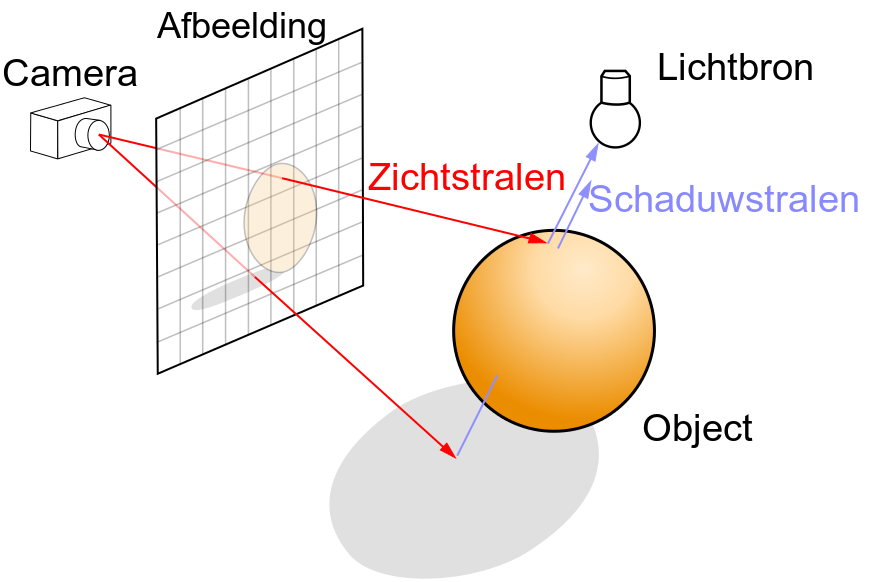
\includegraphics[width=0.5\linewidth]{img/ray-tracing}
    \caption[Visuele voorstelling van \textit{ray tracing}]%
{Visuele voorstelling van \textit{ray tracing} - \small Door elke pixel worden één of meerdere zichtstralen gestuurd. Schaduwstralen worden gebruikt om de belichting in de scene realistisch te maken. Deze afbeelding is een aangepaste versie van een afbeelding op \url{https://en.wikipedia.org/wiki/Ray_tracing_(graphics)}}
    \label{fig:raytracing}    
\end{figure}

Om realistische afbeeldingen te genereren, wordt belichting in het intersectiepunt in rekening gebracht. De eenvoudigste vorm van belichting is directe belichting waarbij een punt donker is als er niet rechtstreeks licht van een lichtbron op valt. Om dit te ondersteunen in \textit{ray tracing} wordt gebruikt gemaakt van schaduwstralen. Dit zijn stralen van het punt naar de lichtbron. Deze schaduwstralen worden geïntersecteerd met de scene, als een intersectiepunt tussen het punt en de lichtbron gevonden wordt, is de lichtbron niet zichtbaar. Bij elke intersectie wordt aan de hand van schaduwstralen gekeken of het punt belicht wordt of niet, als het niet belicht wordt, is de kleur zwart. Voor indirecte belichting - licht dat via reflecties en refracties punten belicht - is \textit{path tracing} \cite{kajiya1986rendering} een veelgebruikte techniek. \textit{Path tracing} reflecteert stralen in het intersectiepunt afhankelijk van het materiaal en als deze straal na een aantal botsingen een lichtbron raakt, krijgt het intersectiepunt een belichting van die lichtbron.    

\paragraph{Acceleratiestructuren}
Het doel van acceleratiestructuren is om de totale tijd nodig om een scene te renderen, te minimaliseren.
Eén van de meest gebruikte representaties van 3D objecten is de \textit{triangle mesh} waarbij het object wordt voorgesteld door een verzameling driehoeken.
De intersectie berekenen tussen een straal en een object komt in dat geval neer op het testen op intersectie tussen de straal en alle driehoeken.
Zelfs een eenvoudige scene kan meer dan honderdduizend driehoeken bevatten en tijdens het renderen kunnen meer dan tien miljoen stralen gestuurd worden.
Het is onhaalbaar om voor elk van deze stralen, elke driehoek op intersectie te testen.
Acceleratiestructuren verminderen de rendertijd door het aantal straal-driehoekintersecties te verminderen.\\

De simpelste acceleratiestructuur bestaat uit het omhullend volume van de scene.
Testen op intersectie met de driehoeken in de scene gebeurt dan enkel als dit omhullend volume intersecteert met de straal.
Deze acceleratiestructuur kan worden uitgebreid tot een boomstructuur door dit volume recursief op te delen in kindvolumes.
Binaire bomen delen elk omhullend volume op in twee nieuwe volumes, andere acceleratiestructuren zoals bijvoorbeeld octrees, delen het volume op in meer dan twee volumes.
\\

Het volume kan worden opgedeeld op twee manieren: volgens objecten of volgens ruimte.
Bij opdeling volgens objecten worden de objecten binnen het volume opgedeeld in meerdere disjuncte groepen en de kindvolumes zijn de omhullende volumes van deze groepen.
Na deze opdeling zit elk object in exact één van deze nieuwe volumes, maar de volumes kunnen overlappen.
Figuur \ref{fig:opdeling-object} toont dit visueel.
Een voorbeeld van een acceleratiestructuur waarbij de opdeling volgens objecten gebeurt is de \textit{Bounding Volume Hierarchy} ($\symBVH$) \cite{goldsmith1987automatic}.
Opdeling volgens ruimte betekent dat de ruimte in het volume wordt opgedeeld in meerdere delen.
Na deze opdeling overlappen deze nieuwe volumes niet, maar een object ligt nu in minstens één (en mogelijks in meerdere) kindvolume(s).
Figuur \ref{fig:opdeling-ruimte} toont dit visueel.
De \textit{Binary Space Partitioning} ($\symBSP$) boom deelt de ruimte van het volume steeds op in twee kindvolumes.
Deze masterproef focust op $\symBSP$ bomen.

\begin{figure}
    \centering
    \begin{subfigure}[t]{0.49\linewidth}
        \centering
    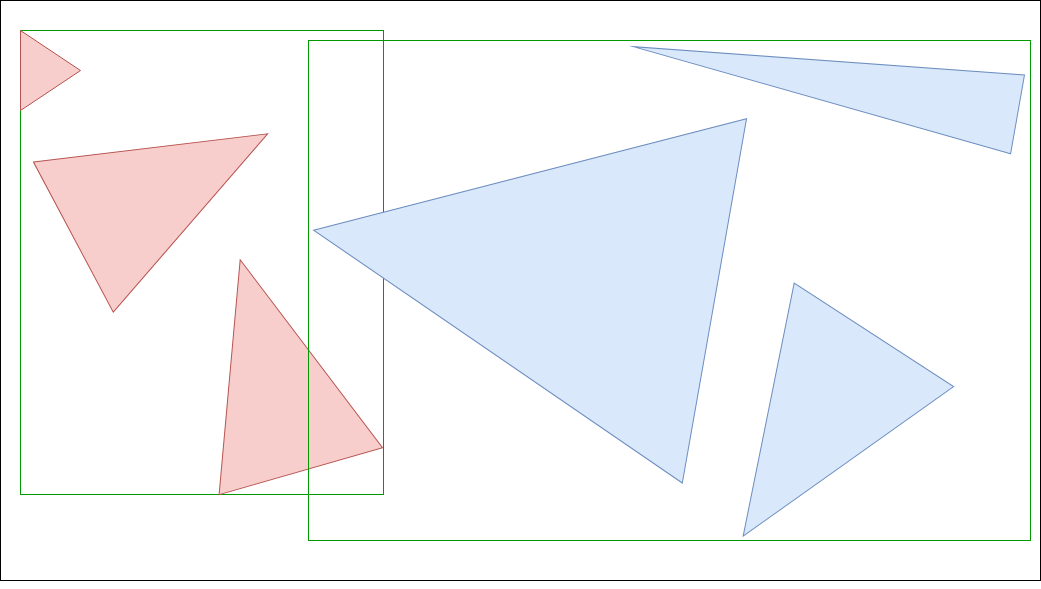
\includegraphics[width=\linewidth]{img/objectSplit}
    \caption{Object}
    \label{fig:opdeling-object} 
    \end{subfigure}
    \begin{subfigure}[t]{0.5\linewidth}
        \centering
    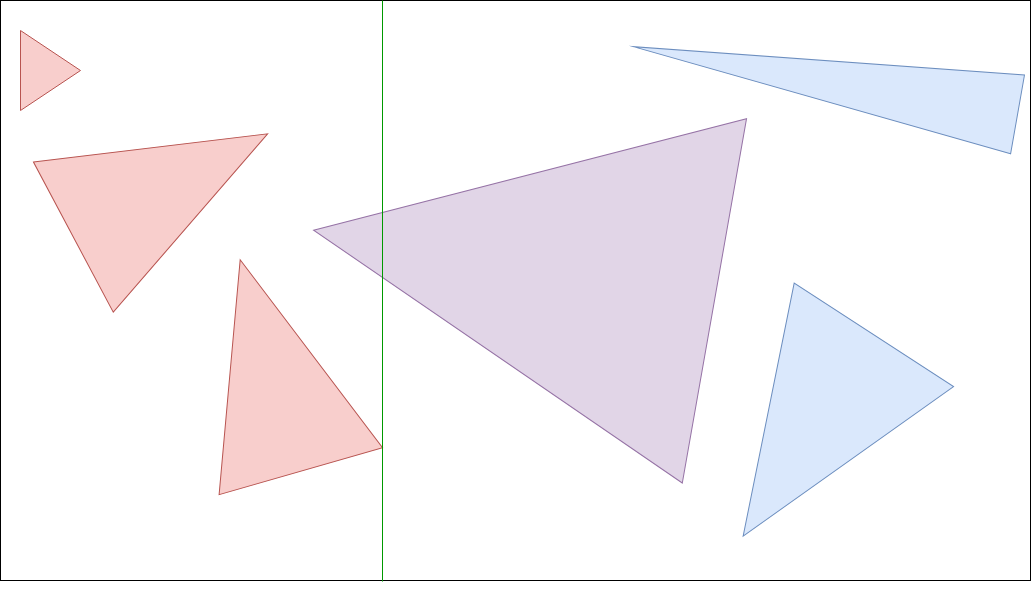
\includegraphics[width=\linewidth]{img/volumeSplit}
    \caption{Ruimte}
    \label{fig:opdeling-ruimte} 
    \end{subfigure}
    \caption[Visuele voorstelling opdeling volume volgens object en ruimte]%
{Visuele voorstelling opdeling volume volgens object en ruimte - \small (a) toont de opdeling volgens object, elk driehoek behoort tot slechts één kindvolume, maar de kindvolumes overlappen. (b) toont de opdeling volgens volume, de paarse driehoek behoort tot beide kindvolumes, maar de kindvolumes zelf zijn disjunct. }
\label{fig:opdeling}
\end{figure}

\section{Doelstelling}
In de praktijk wordt altijd een specifiek soort $\symBSP$ boom gebruikt: de $\symKd$ boom.
Deze boom splitst knopen enkel op via asgealigneerde splitsingsvlakken waardoor hij een aantal computationele voordelen heeft tijdens het bouwen en intersecteren van de boom.
Het nadeel hiervan is dat de $\symKd$ boom zich niet goed kan aanpassen aan complexe niet-asgealigneerde geometrie waardoor bepaalde regio's veel straal-driehoekintersecties nodig hebben.\\

Algemene $\symBSP$ bomen kunnen hiervoor theoretisch gezien een oplossing bieden.
Het ontwerpen van een algemene $\symBSP$ boom die efficiënter is dan de $\symKd$ boom bij het \textit{ray tracen}, is een uitdagend probleem.
Eén van de moeilijkheden bij het bouwen van een algemene $\symBSP$ boom is het kiezen van goede splitsingsvlakken uit het grote aantal mogelijke splitsingsvlakken.
In tegenstelling tot de $\symKd$ boom, waarbij enkel asgealigneerde vlakken mogelijk zijn, zijn alle vlakken mogelijk bij een algemene $\symBSP$ boom.
In deze masterproef wordt onderzocht of het mogelijk is om goede splitsingvlakken te bepalen afhankelijk van de normalen van de driehoeken in de scene.\\

De oplossing die in deze tekst naar voren geschoven wordt, is een nieuw soort algemene $\symBSP$ boom: de $\symBSPsweep$ boom.
De $\symBSPsweep$ boom laat toe om in elke knoop een aantal richtingen te bepalen afhankelijk van de driehoeken in die knoop.
Het beste vlak van alle vlakken met als normaal één van die richtingen, wordt gebruikt om de knoop te splitsen.

\section{Structuur van de tekst}
Hoofdstuk \ref{hoofdstuk:voorgaand-werk} bespreekt de bestaande soorten $\symBSP$ bomen. Hoofdstuk \ref{hoofdstuk:bsp-sweep} start met het beschrijven van het algemene concept van de nieuwe $\symBSPsweep$ boom. Daarna worden drie varianten van dit type boom besproken, één die random richtingen gebruikt en twee die gebruik maken van de normalen. Hoofdstuk \ref{hoofdstuk:implementatie} beschrijft de implementaties, inclusief gelijkenissen en verschillen, van de verschillende bestaande en nieuwe $\symBSP$ bomen. Hoofdstuk \ref{hoofdstuk:resultaten} bespreekt de resultaten van de nieuwe $\symBSPsweep$ bomen in functie van het aantal richtingen en vergelijkt de kwaliteit van de nieuwe bomen met de bestaande $\symBSP$ bomen.

%%% Local Variables: 
%%% mode: latex
%%% TeX-master: "masterproef"
%%% End: 

\chapter{Voorgaand werk}
\label{hoofdstuk:voorgaand-werk}
Raytracing vereist acceleratiestructuren om efficiënt driehoeken in de scene te kunnen zoeken.
Dit hoofdstuk start met een algemene uitleg over acceleratiestructuren en wijdt dan uit over één specifieke acceleratiestructuur: de \textit{Binary Space Partitioning} ($\symBSP$) boom.
De varianten van de $\symBSP$ boom worden één voor één besproken.
% TODO

\section{Acceleratiestructuren}
    Het doel van acceleratiestructuren is om het aantal straal-driehoek intersecties te verminderen.
    De simpelste acceleratiestructuur bestaat uit het omhullende volume van de scene.
    Testen op intersectie met de driehoeken in de scene gebeurt dan enkel als dit omhullende volume intersecteert met de straal.
    Deze acceleratiestructuur kan worden uitgebreid tot een boomstructuur door dit volume recursief op te delen in kindvolumes.
    Binaire bomen delen elk omhullend volume op in twee nieuwe volumes, andere acceleratiestructuren zoals bijvoorbeeld octrees, delen het volume op in meer dan twee volumes.
    \\

    Het volume kan worden opgedeeld op twee manieren: volgens objecten of volgens ruimte.
    Bij opdeling volgens objecten worden de objecten binnen het volume opgedeeld in meerdere disjuncte groepen en de kindvolumes zijn de omhullende volumes van deze groepen.
    Na deze opdeling zit elk object in exact één van deze nieuwe volumes, maar de volumes kunnen overlappen.
    Een voorbeeld van een acceleratiestructuur waarbij de opdeling volgens objecten gebeurt is de \textit{Bounding Volume Hierarchy} ($\symBVH$).
    Opdeling volgens ruimte betekent dat de ruimte in het volume wordt opgedeeld in meerdere delen.
    Na deze opdeling overlappen deze nieuwe volumes niet, maar een object ligt nu in minstens één (en mogelijks in meerdere) kindvolume(s).
    De $\symBSP$ boom deelt de ruimte van het volume steeds op in twee kindvolumes.
    % TODO: combinatie van Kd en BVH ? SBVH
    % TODO: check if all abbrev are listed and defined at first usage

\section{$\symBSP$ bomen}
    De $\symBSP$ boom deelt de ruimte van het omhullende volume recursief op door te splitsen volgens een willekeurig georiënteerd vlak totdat een bepaalde stopconditie bereikt is.
    Het feit dat de $\symBSP$ volgens willekeurig georiënteerde vlakken splitst, is zowel een voor- als een nadeel.
    Het zorgt ervoor dat de $\symBSP$ zich heel goed kan aanpassen aan de scene en alle niet-intersecterende driehoeken in principe kan scheiden.
    Maar het zorgt er ook voor dat het heel moeilijk is om deze goede splitsingsvlakken te vinden.
    In de praktijk wordt vaak een specifieke soort $\symBSP$ boom gebruikt: de $\symKd$ boom.
    
    \paragraph{Het bouwen van de boom}
    Het splitsingsvlak dat een knoop opdeelt in twee delen, kan een grote impact hebben op het aantal doorkruisstappen en het aantal driehoekintersecties.
    Het bouwalgoritme moet voor elke knoop het beste splitsingvlak bepalen en als splitsen volgens dat vlak voordelig is, de knoop opsplitsen in twee kindknopen.
    Heuristieken voorspellen hoe goed een splitsing volgens een bepaald splitsingsvlak is.   
    Het algoritme stopt met het splitsen van de knoop als het aantal driehoeken in de knoop lager is dan een vastgelegde limiet, bijvoorbeeld als er maar één driehoek in de knoop zit.

    %Spatiaal, opsplitsen volgens willekeurige vlakken
    %Niet feasible geacht
   
\section{$\symKd$ Bomen}   
    De $\symKd$ boom is een $\symBSP$ boom waarbij alle splitsingsvlakken asgealigneerd zijn.
    Hiermee wordt bedoeld dat de splitsingsrichting (de normaal op het splitsingsvlak) evenwijdig is aan één van de drie hoofdassen.
    Dit zorgt ervoor dat elke knoop van de boom een asgealigneerde balk voorstelt.
    Het doorkruisen van een knoop uit een $\symKd$ boom is daardoor goedkoper dan het doorkruisen van een knoop uit een algemene $\symBSP$ boom.
    De reden hiervoor is dat het goedkoper is om het intersectiepunt van een straal en een asgealigneerd vlak te vinden (verschil en vermenigvuldiging) dan het intersectiepunt van een straal en een willekeurig vlak (scalair product en deling).
    Door de beperking op mogelijke splitsingsvlakken kunnen $\symKd$ bomen zich minder goed aanpassen aan de scene.
    Ze kunnen bijvoorbeeld niet alle niet-intersecterende driehoeken scheiden. 
    \\ % TODO: 2D voorbeeld van splitsbaar en wat niet

    Ondanks dit nadeel, worden in de praktijk $\symKd$ bomen verkozen boven algemene $\symBSP$ bomen.
    \authorIze{} \cite{ize} geven drie (volgens hun foute) ruimverspreide aannames over algemene $\symBSP$ bomen die ervoor zorgen dat $\symKd$ bomen hoger ingeschat worden.
    Ten eerste wordt er aangenomen dat algemene $\symBSP$ bomen nooit sneller kunnen zijn dan $\symKd$ bomen omdat het doorkruisen van een $\symBSP$ boom beduidend duurder is.
    De beperkte precisie van vlottende komma getallen wordt gezien als het tweede probleem omdat het $\symBSP$ bomen numeriek onstabiel zou maken.
    De derde aanname is dat door de grotere flexibileit (= grotere verzameling van mogelijke splitsingsvlakken) het veel moeilijker is om een $\symBSP$ boom te bouwen dan om een $\symKd$ boom te bouwen.
    \\

    Voor een Kd-boom is de Surface Area Heuristiek (SAH) de beste gekende methode om bomen met minimale verwachtte kost te bouwen.
    De $\symSAH$ is oorspronkelijk ontwikkelt door REF voor de $\symBVH$ en later aangepast door REF voor de $\symKd$ boom. 
    De $\symSAH$ schat de kost van een splitsingsvlak door te veronderstellen dat beide kindknopen bladknopen worden. 
    De verwachte kost $\symCost$ om een knoop $\symNodeExample$ te splitsen in kindknopen ${\symLeft}$ en ${\symRight}$ is dan: $\symCost_\symNodeExample = \frac{\symSA(\symLeft)}{\symSA(\symNodeExample)}*\symNbPrimitives_\symLeft*\symCost_\symIntersection + \frac{\symSA(\symRight)}{\symSA(\symNodeExample)}*\symNbPrimitives_\symRight*\symCost_\symIntersection + \symCost_\symTraversal$ met kost $\symCost$, oppervlakte $\symSA()$ en aantal driehoeken $\symNbPrimitives$.
    De subscripts ${\symIntersection}$ en ${\symTraversal}$ staan voor respectievelijk intersectie en doorkruising.

    SAH (inclusief nulbonus) -> sweeping
\section{RBSP-bomen}
    De Restricted Binary Space Partitioning ($\symRBSP$) boom is een uitbreiding van de $\symKd$ boom ontwikkeld door \authorKammaje{ } \cite{Kammaje}.
    De $\symRBSP$ boom laat toe om knopen op te splitsen volgens splitsingsrichtingen uit een vaste verzameling richtingen.
    Deze splitsingsrichtingen moeten niet asgealigneerd zijn.
    \authorKammaje{ } stellen de richtingen %TODO
    Het omhullend volume van een $\symRBSP$ knoop is hierdoor geen balk maar een Discreet Geöriënteerde Polytoop met k richtingen: een $\symKDOP$. %TODO: check kDOP
    \authorKammaje{ } toonden aan dat de SAH ook gebruikt kan worden voor $\symRBSP$ bomen. Het berekenen van de oppervlakte van een $\symKDOP$ is computationeel duurder dan het berekenen van de oppervlakte van een balk. Het doorkruisen van een $\symRBSP$ knoop is duurder dan het doorkruisen van een $\symKd$ knoop.
    %TODO: Budge -> incrementele oppervlakte berekening
    \\

    Huidige $\symRBSP$ implemenaties moeten onderdoen voor de $\symKd$ bomen. \authorIze{ } menen dat de $\symRBSP$ boom de slechtste eigenschappen van zowel de $\symKd$ boom als de algemene $\symBSP$ boom overneemt. Net als de $\symKd$ boom kan het geen rekening houden met de lokale geometrie en zich dus niet aanpassen aan complexe geometrie. Net als bij de algemene $\symBSP$ boom moet de intersectie met een willekeurig georiënteerd vlak berekend worden om knopen te doorkruisen.

    Algemener dan Kd -> meer richtingen -> richtingen gekozen volgens
    kDOPs ipv balken

\section{Algemene BSP-Bomen in de praktijk}
    \authorIze{ } ontwikkelde de eerste algemene $\symBSP$ boom voor raytracing \cite{ize}. In teenstelling
    Paper Ize et al.
        3 Kd richtingen (sweepen) plus 4 richtingen afhankelijk van geometrie 
        Snelle Kd traversal, aanpassing SAH
        Geen sweeping -> BVH als hulpstructuur
    
    Voordelen
        Knopen kunnen beter worden opgesplist
    Nadelen
        Duurder om te traversen
        Duurder om te bouwen (berekening SA van veelvlak vs SA van balk)
        Grote zoekruimte om beste splitsingsvlak te vinden
 
\section{Hiërarchie}
\paragraph{Aantal verschillende splitsingsvlakken}
Eén van de belangrijkste eigenschappen van een $\symBSP$ algoritme is zijn vermogen om zich aan te passen aan complexe geometrie.
Het totaal aantal verschillende splitsingsvlakken dat bekeken wordt tijdens het bouwen van de boom, draagt bij tot dit vermogen.
Voor een scene met $n$ driehoeken, bekijkt een $\symKd$ boom $6n$ verschillende splitsingsvlakken. 
Elk niveau van de boom bekijkt exact dezelfde splitsingsvlakken.
Een $\symRBSP$ boom met k discrete richtingen doet hetzelfde, maar bekijkt $2kn$ verschillende splitsingsvlakken. 
De $\symBSPize$ boom gebruikt $10n$ verschillende splitsingsrichtingen, $6n$ voor de $\symKd$ richtingen en $n$ voor elk van de vier andere richtingen.
De $\symBSPize$ boom bekijkt op elk niveau ook exact dezelfde splitsingvlakken en is dus niet zo algemeen als een $\symBSP$ boom kan zijn. 
De reden hiervoor is dat de gebruikte $\symBSP$ splitsingsvlakken enkel afhankelijk zijn van de driehoeken zelf en niet van welke driehoeken samen in een knoop zitten.
Geen van bovenstaande bomen gebruikt de volledige vrijheid van een $\symBSP$ boom om op elk niveau andere splitsingsvlakken te nemen en op die manier beperken ze hun vermogen om zich aan te passen aan complexe geometrie.

%%% Local Variables: 
%%% mode: latex
%%% TeX-master: "masterproef"
%%% End: 

\chapter{$\mathbf{\symBSPsweep}$}
\label{hoofdstuk:bsp-sweep}
In dit hoofdstuk wordt een nieuw soort $\symBSP$ boom besproken: de $\symBSPsweep$ boom.
Eerst wordt het nut van het opsplitsen van bladknopen in kleinere bladknopen wiskundig besproken en aangetoond met behulp van een voorbeeld.
Het algemene idee van de $\symBSPsweep$ boom wordt dan besproken en daarna worden een aantal specifieke versies van de $\symBSPsweep$ ($\symBSPrandom$, $\symBSParbitrary$ en $\symBSPcluster$) besproken.

\section{Probleemstelling}
    Het doel van acceleratiestructuren is om de totale tijd nodig om een scene te renderen, te minimaliseren.
    Deze sectie toont aan dat de totale rendertijd afhankelijk is van het aantal driehoeken in de geïntersecteerde bladknopen.
    In de eerste subsectie wordt wiskundig aangetoond dat het (onder bepaalde aannames) altijd voordelig is om bladknopen met meer dan één driehoek op te splitsen in kleinere bladknopen.
    De tweede subsectie toont een voorbeeld waarbij de $\symKd$ en $\symBSPize$ boom vergeleken worden op basis van de grootte van de bladknopen.
\subsection{Wiskundige basis}
    De rendertijd $\symTime_{\symRender}$ bestaat uit twee grote factoren: de tijd gespendeerd aan het intersecteren met driehoeken (de intersectietijd) en de tijd gespendeerd aan het doorkruisen van de boom (de doorkruistijd).
    De totale intersectietijd $\symTime_{\symIntersection, \symTotal}$ is afhankelijk van het aantal driehoeken $\symNbPrimitives_\symLeaf$ in de geïntersecteerde bladknopen $\symLeaf$ en het aantal keer $\symTraversalL_\symLeaf$ dat elk van deze bladknopen doorkruist wordt.
    De totale doorkruistijd $\symTime_{\symTraversal, \symTotal}$ is afhankelijk van het aantal doorkruisingen $\symTraversalL_{\symInternal}$ van inwendige knopen.
    Formule \ref{eq:rendertijd} beschrijft dit wiskundig met $\symTime_{\symIntersection}$ de tijd nodig voor één straal-driehoekintersectie, $\symTime_{\symTraversal}$ de tijd nodig om één knoop te doorkruisen en $B$ het aantal geïntersecteerde bladknopen.
\begin{equation}
    \label{eq:rendertijd}
   \symTime_{\symRender} \sim
    \symTime_{\symIntersection, \symTotal} + \symTime_{\symTraversal, \symTotal} = \symTime_{\symIntersection} * \sum_{\symLeaf}^\symLeafL \symNbPrimitives_\symLeaf * \symTraversalL_\symLeaf + \symTime_{\symTraversal} * \symTraversalL_{\symInternal}
\end{equation}

Stel dat één kindknoop $\symLeaf_j$ uit de boom wordt opgesplitst in twee kleinere kindknopen $\symLeaf_{j1}$ en $\symLeaf_{j2}$ die elk de helft van de driehoeken krijgen.
Deze opsplitsing is voordelig als aan voorwaarde \ref{eq:vw_splitwinst} voldaan is.
Deze voorwaarde drukt uit dat knoop $\symLeaf_j$ nu een inwendig knoop wordt en dus niet meer zorgt voor een intersectietijd en wel voor een doorkruistijd en dat de nieuwe kindknopen zorgen voor een intersectietijd.
De voorwaarde is equivalent aan voorwaarden \ref{eq:vw_splitwinst_tussen} en \ref{eq:vw_splitwinst_res}.
% B -> 2Bs : nb -> nb/2 * 2 en Db1 + db2 << Db + 1 inwendige knoop, Db keer bekeken
\begin{equation}
    \label{eq:vw_splitwinst}
    \symTime_{\symRender} - \symTime_{\symIntersection} * \symNbPrimitives_{\symLeaf_j} * \symTraversalL_{\symLeaf_j} + \symTime_{\symTraversal} * \symTraversalL_{\symLeaf_j}  + \frac{\symNbPrimitives_{\symLeaf_j}}{2} * (\symTraversalL_{\symLeaf_{j1}} + \symTraversalL_{\symLeaf_{j2}}) * \symTime_{\symIntersection} \leq \symTime_{\symRender}
\end{equation}
\begin{equation}
    \label{eq:vw_splitwinst_tussen}
  \Leftrightarrow \frac{\symNbPrimitives_{\symLeaf_j}}{2} * (\symTraversalL_{\symLeaf_{j1}} + \symTraversalL_{\symLeaf_{j2}}) * \symTime_{\symIntersection} \leq (\symTime_{\symIntersection} * \symNbPrimitives_{\symLeaf_j} - \symTime_{\symTraversal}) * \symTraversalL_{\symLeaf_j}
\end{equation}
%\begin{equation}
%    \frac{\symNbPrimitives_{\symLeaf_j} * \symTime_{\symIntersection}}{(\symTime_{\symIntersection} * \symNbPrimitives_{\symLeaf_j} - \symTime_{\symTraversal})} \leq \frac{2\symTraversalL_{\symLeaf_j}}{(\symTraversalL_{\symLeaf_{j1}} + \symTraversalL_{\symLeaf_{j2}}) }
%\end{equation}
%\begin{equation}
%    \frac{1}{(1 - \frac{\symTime_{\symTraversal}}{\symNbPrimitives_{\symLeaf_j} * \symTime_{\symIntersection}})} \leq \frac{2\symTraversalL_{\symLeaf_j}}{(\symTraversalL_{\symLeaf_{j1}} + \symTraversalL_{\symLeaf_{j2}}) }
%\end{equation}
\begin{equation}
    \label{eq:vw_splitwinst_res}
    \Leftrightarrow \symTraversalL_{\symLeaf_{j1}} + \symTraversalL_{\symLeaf_{j2}} \leq
    2\symTraversalL_{\symLeaf_j} * (1 - \frac{\symTime_{\symTraversal}}{\symNbPrimitives_{\symLeaf_j} * \symTime_{\symIntersection}})
\end{equation}

De som in het linkerlid van voorwaarde \ref{eq:vw_splitwinst_res} is minstens gelijk aan $\symTraversalL_{\symLeaf_{j}}$ aangezien elke doorkruising van $\symLeaf_j$ voor minstens één doorkruising door een kindknoop zorgt.
Analoog kan worden ingezien dat de maximale waarde voor deze som gelijk is aan $2\symTraversalL_{\symLeaf_{j}}$ aangezien elke doorkruising van $\symLeaf_j$ voor maximaal twee doorkruisingen door een kindknoop kan zorgen. Hieruit volgt ongelijkheid \ref{eq:vw_doorkruisingen}.

\begin{equation}
    \label{eq:vw_doorkruisingen}
    \symTraversalL_{\symLeaf_{j}} \leq \symTraversalL_{\symLeaf_{j1}} + \symTraversalL_{\symLeaf_{j2}} \leq 2\symTraversalL_{\symLeaf_{j}}
\end{equation}

In het algemeen geval geldt dat $\symTraversalL_{\symLeaf_{j1}} + \symTraversalL_{\symLeaf_{j2}} = (2 * (1-\beta) + \beta) \symTraversalL_{\symLeaf_{j}}$ waarbij $\beta$ het procentueel aantal doorkruisingen is dat door slechts één van de twee kindknopen gaat.
In dit geval leidt voorwaarde \ref{eq:vw_splitwinst_res} tot voorwaarde \ref{eq:vw_splitwinst_general}.
\begin{equation}
    \label{eq:vw_splitwinst_general}
    (2 * (1-\beta) + \beta) \symTraversalL_{\symLeaf_{j}} \leq
    2\symTraversalL_{\symLeaf_j} - \frac{2\symTraversalL_{\symLeaf_j}\symTime_{\symTraversal}}{\symNbPrimitives_{\symLeaf_j} \symTime_{\symIntersection}}
    \Leftrightarrow
    2 - \beta \leq 2 - \frac{2\symTime_{\symTraversal}}{\symNbPrimitives_{\symLeaf_j} \symTime_{\symIntersection}}
    \Leftrightarrow
    \symTime_{\symTraversal} \leq \frac{\beta \symNbPrimitives_{\symLeaf_j} }{2}\symTime_{\symIntersection}
\end{equation}

In het ideale geval ($\beta = 1$) leidt voorwaarde \ref{eq:vw_splitwinst_general} tot $\symTime_{\symTraversal} \leq \frac{\symNbPrimitives_{\symLeaf_j}}{2}\symTime_{\symIntersection}$.
Het opsplitsen van een knoop met twee driehoeken, kan hierdoor pas voordelig zijn als de doorkruistijd kleiner is dan de intersectietijd.
Aangezien de doorkruistijd in de realiteit beduidend kleiner is dan de intersectietijd, is het in dit ideale geval altijd voordelig om een kindknoop op te splitsen, ongeacht het aantal driehoeken in de knoop.
In het slechtste geval ($\beta = 0$) kan aan voorwaarde \ref{eq:vw_splitwinst_general} enkel voldaan zijn als de doorkruistijd gelijk is aan nul. Dit is onmogelijk waardoor opsplitsen nooit voordelig kan zijn in dit geval. \\

Het is moeilijk om de waarde van $\beta$ te voorspellen, deze is namelijk afhankelijk van de exacte stralen die tijdens het renderen gevolgd worden, de specifieke driehoeken in de knoop en het splitsingsvlak. 
Voorwaarde \ref{eq:vw_splitwinst_general} toont dat de kans dat splitsen voordelig is, lineair stijgt met $\symNbPrimitives_{\symLeaf_j}$. 
De voorwaarde toont ook dat het splitsen van een knoop met twee driehoeken, voordelig is wanneer de doorkruistijd $\beta$ keer kleiner is dan de intersectietijd. 
Intuïtief lijkt het logisch dat hier in het algemeen aan voldaan is. 
Hieruit kan worden afgeleid dat het altijd beter is om bladknopen met meer dan één driehoek op te splitsen in twee kleinere bladknopen.\\

\subsection{Voorbeeld}
  \begin{figure}
    \begin{subfigure}{0.4\textwidth}
        \centering
        \begin{subfigure}{\textwidth}
            \centering
            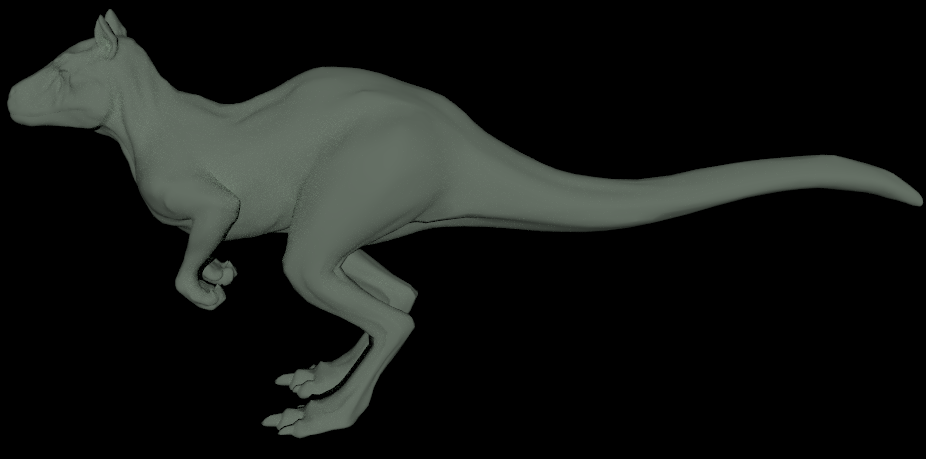
\includegraphics[width=1\linewidth]{img/killeroo}
            \caption{Killeroo scene}
            \label{fig:killeroo}    
        \end{subfigure}
        \begin{subfigure}{\textwidth}
            \centering
            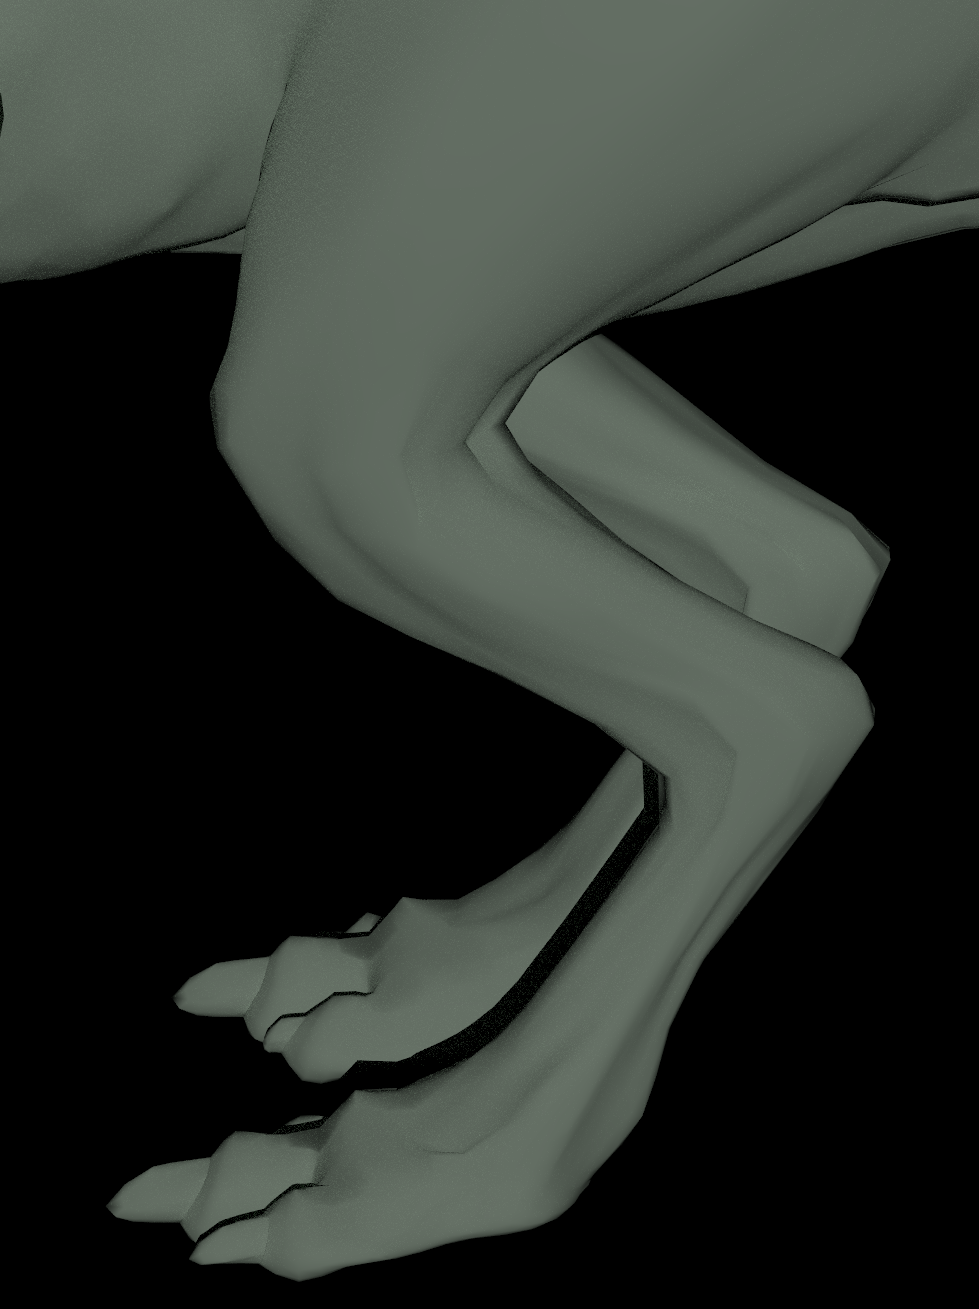
\includegraphics[width=0.5\linewidth]{img/killerooFeet}
            \caption{Killeroo Been scene}
            \label{fig:killeroo-been}    
        \end{subfigure}
    \end{subfigure}
    \begin{subfigure}{0.5\textwidth}
        \centering
    \begin{tikzpicture}[scale=0.6]
        \begin{axis}[
          axis lines = left,
          ylabel = \small Cumulatieve bijdrage aan totaal aantal straal-driehoekintersecties,
          xlabel = \small Aantal driehoeken in bladknoop,
          ymin=1000000, ymax=180000000,
          width=1.6\textwidth,
          height=2\textwidth,
          cycle multi list={%
            color list\nextlist
            [2 of]mark list
          },
          title = \small,
          legend pos=north west,
      ]
        \addplot table [x=V1, y=KillerooKdTotal, col sep=comma] {data/killeroo_feet_kd_bsp.csv};
        \addlegendentry{$\symKd$ Killeroo}
        \addplot table [x=V1, y=FeetKdTotal, col sep=comma] {data/killeroo_feet_kd_bsp.csv};
        \addlegendentry{$\symKd$ Killeroo Been}
    
        \addplot table [x=V1, y=KillerooBSPTotal, col sep=comma] {data/killeroo_feet_kd_bsp.csv};
        \addlegendentry{$\symBSPizefastkd$ Killeroo}
        \addplot table [x=V1, y=FeetBSPTotal, col sep=comma] {data/killeroo_feet_kd_bsp.csv};
        \addlegendentry{$\symBSPizefastkd$ Killeroo Been}
        
          \end{axis}
        \end{tikzpicture}
        \caption{Cumulatief aantal straal-driehoekintersecties}
        \label{fig:voorbeeld-cumul}
    \end{subfigure}
    \label{fig:voorbeeld-bladknopen}
    \caption[Invloed grootte bladknopen op het aantal straal-driehoekintersecties]{Invloed grootte bladknopen op het aantal straal-driehoekintersecties - \small (a) toont de Killeroo scene, (b) toont de scene waarbij ingezoomd is op de benen van de Killeroo, (c) toont het totaal aantal intersecties als een cumulatieve som over het aantal driehoeken in de bladknoop. Dit betekent dat de waarde bij x overeenkomt met de som van het aantal intersecties in bladknopen met x of minder driehoeken.}
\end{figure}
Figuur \ref{fig:killeroo} toont de Killeroo scene die als voorbeeld scene dient bij de pbrt \cite{pbrt} \textit{ray tracer}.
Voor deze scene zijn de $\symKd$ boom en de $\symBSPizefastkd$ boom aan elkaar gewaagd.
De $\symBSPizefastkd$ boom neemt de bovenhand als er wordt ingezoomd op de benen (figuur \ref{fig:killeroo-been}) van de Killeroo, waar de $\symKd$ boom veel bladknopen met meerdere driehoeken bevat.
Figuur \ref{fig:voorbeeld-cumul} toont het cumulatief aantal intersecties per groep van bladknopen met hetzelfde aantal driehoeken.
Voor de gewone Killeroo scene, heeft de $\symKd$ boom slechts een beperkt aantal extra intersecties nodig.
Bij de ingezoomde scene, komt een groot deel van de intersecties van de $\symKd$ boom door intersecties met bladknopen met een groot aantal driehoeken.
Dit toont aan dat algemene $\symBSP$ bomen nuttig kunnen zijn omdat ze in principe alle niet-intersecterende driehoeken van elkaar kunnen scheiden en er dus minder regio's zijn met veel grote bladknopen.
Het aantal knoopdoorkruisingen bij de $\symBSPizefastkd$ boom is zelfs lager dan bij de $\symKd$ boom voor beide scenes.
Dit komt omdat de algemene $\symBSP$ bomen nauwer aansluiten aan het object waardoor minder stralen de knopen raken.\\

Figuur \ref{fig:killeroo-heatmaps} toont \textit{false color} afbeeldingen van het aantal zichtstraalintersecties van de Killeroo en Killeroo Been scene voor zowel de $\symKd$ boom als de $\symBSPizefastkd$ boom. 
Voor de Killeroo scene zijn de \textit{false color} afbeeldingen van beide bomen zeer gelijkaardig, maar aan de benen heeft de $\symKd$ boom duidelijk meer intersecties nodig.
Dit wordt bevestigd door de \textit{false color} afbeeldingen van de Killeroo Been scene waarop duidelijk zichtbaar is dat de $\symBSPizefastkd$ boom zich beter kan aanpassen aan complexe geometrie.
Het is ook zichtbaar dat de $\symBSPizefastkd$ boom nauwer aansluit aan de scene dan de $\symKd$ boom.
Merk op dat, zoals besproken in het vorige hoofdstuk, de $\symBSPizefastkd$ boom nog niet alle vrijheiden van een algemene $\symBSP$ boom gebruikt.\\

\begin{figure}
    \begin{subfigure}{0.5\textwidth}
        \centering
        \begin{subfigure}{\textwidth}
            \centering
            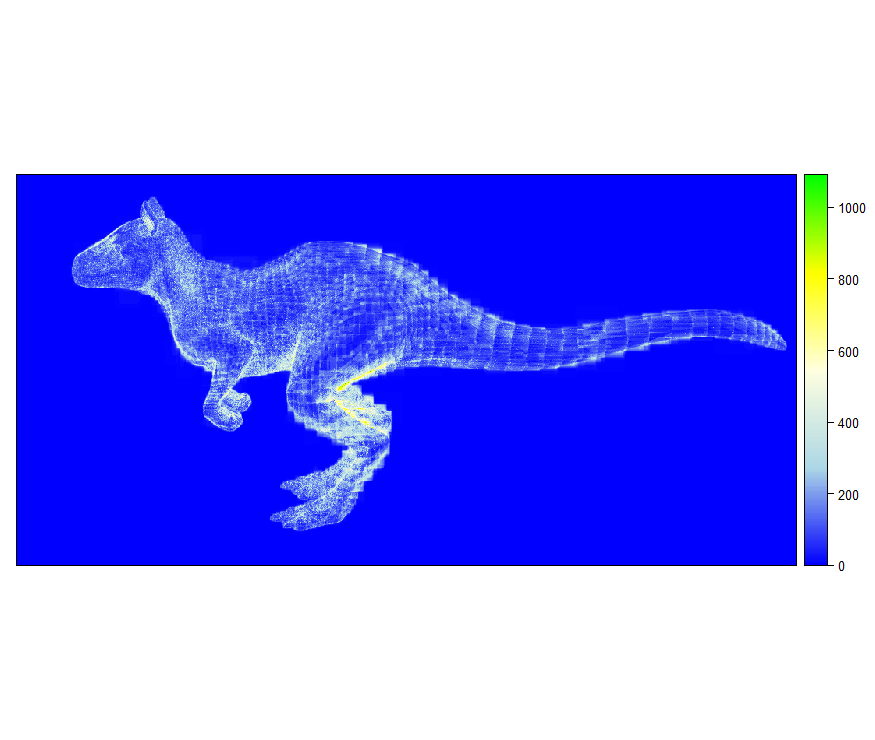
\includegraphics[width=1\linewidth]{img/killeroo-kd-heatmap}
            \caption{Killeroo $\symKd$}
            \label{fig:killeroo-kd-heatmap}    
        \end{subfigure}
        \begin{subfigure}{\textwidth}
            \centering
            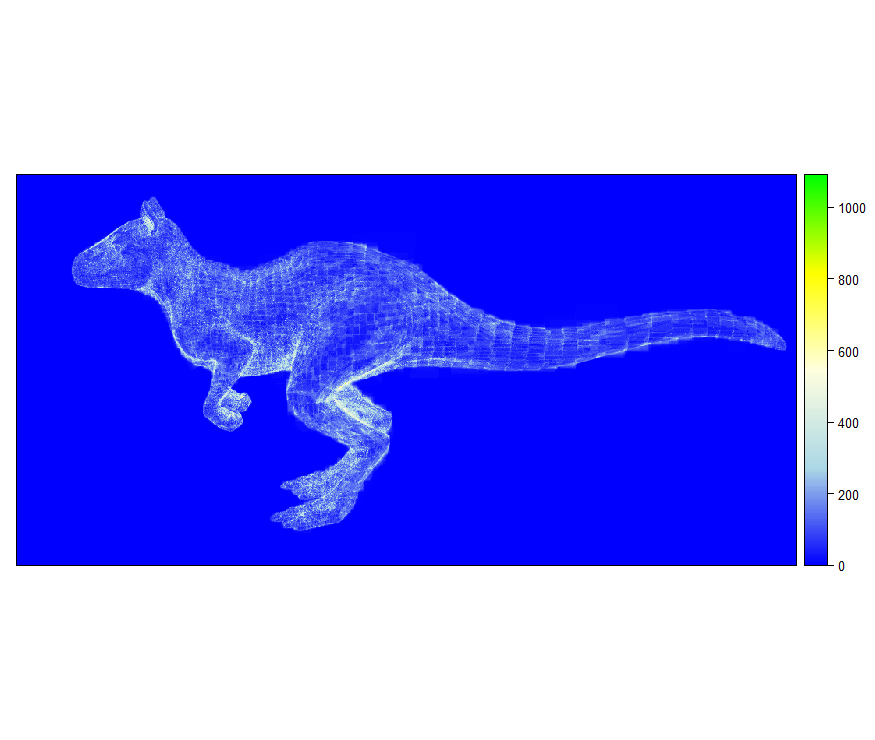
\includegraphics[width=1\linewidth]{img/killeroo-bspize-heatmap}
            \caption{Killeroo $\symBSPizefastkd$}
            \label{fig:killeroo-bspize-heatmap}    
        \end{subfigure}
    \end{subfigure}
    \begin{subfigure}{0.5\textwidth}
        \centering
        \begin{subfigure}{\textwidth}
            \centering
            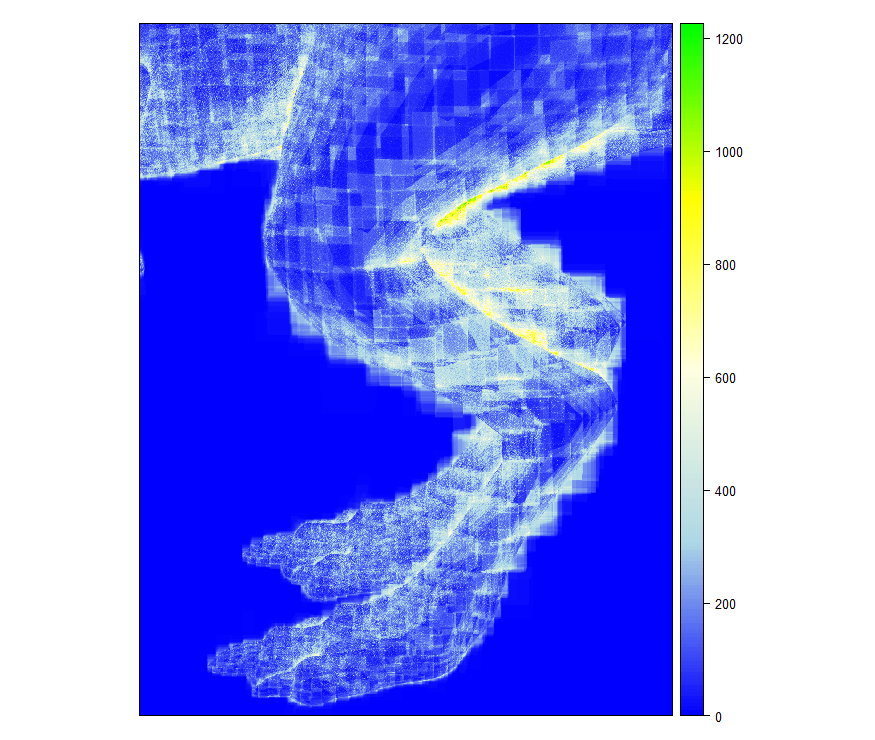
\includegraphics[width=1\linewidth]{img/killeroo-feet-kd-heatmap}
            \caption{Killeroo Been $\symKd$}
            \label{fig:killeroo-been-kd-heatmap}    
        \end{subfigure}
        \begin{subfigure}{\textwidth}
            \centering
            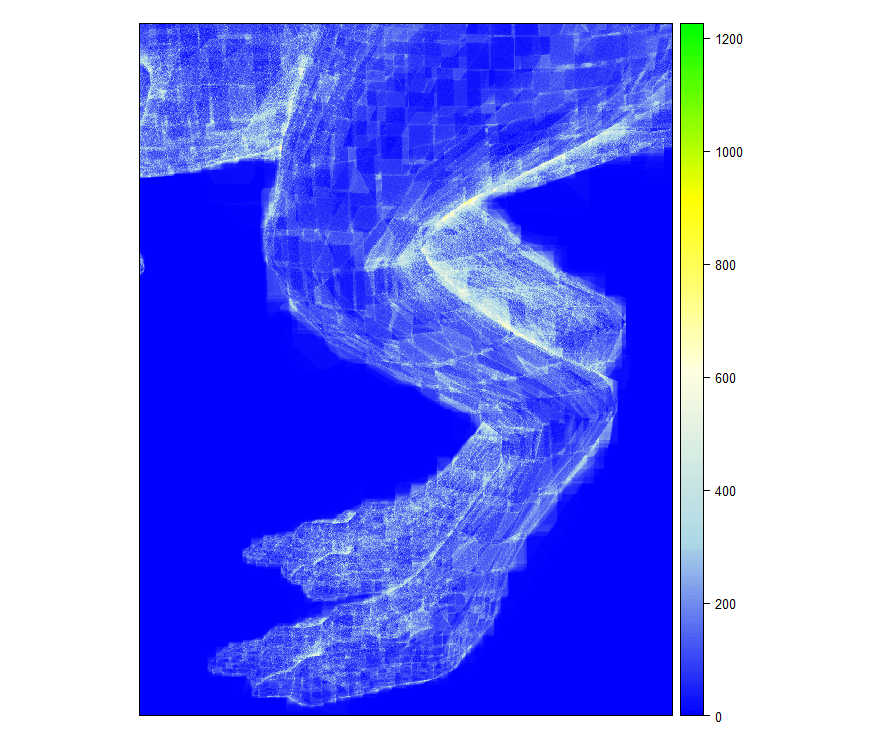
\includegraphics[width=1\linewidth]{img/killeroo-feet-bspize-heatmap}
            \caption{Killeroo Been $\symBSPizefastkd$}
            \label{fig:killeroo-been-bspize-heatmap}    
        \end{subfigure}
    \end{subfigure}
    \caption[\textit{False color} afbeeldingen van de Killeroo en Killeroo Been scene]{\textit{False color} afbeeldingen van de Killeroo en Killeroo Been scene - \small Deze afbeeldingen tonen dat de $\symKd$ boom slecht presteert bij sommige delen van een scene, in dit geval de benen van de Killeroo. Bij de $\symBSPizefastkd$ boom is dit fenomeen veel minder uitgesproken en het valt ook op dat de $\symBSPizefastkd$ boom nauwer aansluit aan de scene.}
    \label{fig:killeroo-heatmaps}
\end{figure}

De volgende secties bespreken nieuwe $\symBSP$ bomen die gebruik maken van de vrijheid om op elk niveau van de boom andere splitsingsvlakken te gebruiken. Op die manier kunnen ze meer bladknopen opsplitsen in kleinere bladknopen en nog nauwer aansluiten aan de scene.\\



\section{Basisidee}
    De $\symBSPsweep$ boom is een algemene $\symBSP$ boom waarbij in elke knoop k richtingen bepaald worden en alle $2n$ splitsingsvlakken langs elk van deze richtingen worden bekeken door te sweepen.
    Deze k richtingen kunnen verschillend zijn voor elke knoop en kunnen gekozen worden afhankelijk van de lokale geometrie.
    De $\symRBSP$ boom is een $\symBSPsweep$ boom waarbij de gekozen richtingen in elke knoop hetzelfde zijn.
    De $\symBSPsweep$ boom heeft drie belangrijke ontwerpbeslissingen.
    De belangrijkste ontwerpbeslissing bij de $\symBSPsweep$ boom is de methode die gebruikt wordt om de k richtingen te bepalen.
    Een tweede belangrijke ontwerpbeslissing is de waarde van k.
    De derde belangrijke ontwerpbeslissing sluit aan bij de eerste en gaat over het al dan niet gebruiken van de $\symKd$ richtingen als de eerste drie van de k richtingen.
    \\


    %Kd-richtingen + aantal richtingen of puur die richtingen
    %Snelle traversal voor kd-richtingen
\section{Gebaseerd op random richtingen}
De simpelste $\symBSPsweep$ boom, de $\symBSPrandom$ boom, bepaalt in elke knoop k random richtingen onafhankelijk van de geometrie.
De richtingen worden uniform op de hemisfeer gegenereerd.
Het idee achter deze boom is dat het nuttiger kan zijn om driehoeken via veel verschillende vlakken te proberen splitsen, dan om ze steeds met dezelfde vlakken te proberen splitsen.
Als de driehoeken in de scene uniform verdeeld zijn, dan is de kans dat twee driehoeken volgens een willekeurige richting gesplitst kunnen worden, even groot als de kans dat ze door een $\symKd$ richting gesplitst kunnen worden.\\

Als de $\symBSPrandom$ boom perfect gebalanceerd is, worden in elk niveau $2kn$ verschillende splitsingsvlakken bekeken.
Deze splitsingsvlakken zijn verschillend op elk niveau, zodat in totaal $2knlog(n)$ verschillende splitsingsvlakken bekeken worden.
Figuur \ref{fig:splitsingsvlakken-bsprandom} toont dit visueel.
De $\symBSPrandom$ boom probeert elke driehoek via gemiddeld $2klog(n)$ ($\symO(log(n))$) vlakken te splitsen van de andere driehoeken, in tegenstelling tot de bestaande bomen die dit maximaal met $\symO(1)$ vlakken proberen.\\

\begin{figure}
    \centering

   \resizebox{0.4\textwidth}{!}{%
   \centering
    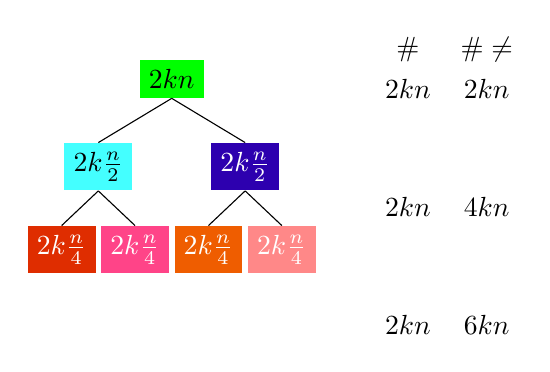
\begin{tikzpicture}
   \Tree
   [ .\node[fill=green]{$2kn$};    
       [.\node[fill=nodeblue1]{$2k\frac{n}{2}$};
           [.\node(n3l)[fill=nodered1, text=white]{$2k\frac{n}{4}$};]
           [.\node[fill=nodered2, text=white]{$2k\frac{n}{4}$};]
       ]
       [.\node[fill=nodeblue2, text=white]{$2k\frac{n}{2}$};
           [.\node[fill=nodered3, text=white]{$2k\frac{n}{4}$};]
           [.\node(n3r)[fill=nodered4, text=white]{$2k\frac{n}{4}$};]
       ]
   ]
   \node at (3,0.5) {$\#$};
   \node at (4,0.5) {$\# \neq$};
   \node at (3,0) {$2kn$};
   \node at (3,-1.5) {$2kn$};
   \node at (3,-3) {$2kn$};
   \node at (4,0) {$2kn$};
   \node at (4,-1.5) {$4kn$};
   \node at (4,-3) {$6kn$};
   \end{tikzpicture}
   }
   \caption[Splitsingsvlakken $\symBSPrandom$]%
    {Splitsingsvlakken $\symBSPrandom$ - \small Per niveau het aantal ($\#$) splitsingsvlakken en het totaal aantal verschillende ($\# \neq$) splitsingsvlakken gebruikt in bovenliggende niveaus bij de $\symBSPrandom$ boom.} %TODO: meer uitleg
    \label{fig:splitsingsvlakken-bsprandom}
\end{figure}

\begin{figure}
        \resizebox{\textwidth}{!}{%
        \centering
         \begin{tikzpicture}
            \usetikzlibrary{arrows}
            \usetikzlibrary{shapes}
\tikzstyle{every tree node}=[draw, ellipse, align=center]
        \Tree
        [ .\node[shading = axis, left color=green, right color=nodeyellow1,shading angle=135]{$2(k-3)n + 6n$};    
            [.\node[shading = axis, left color=nodeblue1, right color=nodeyellow1, shading angle=135]{$2(k-3)\frac{n}{2} + 6\frac{n}{2}$};
                [.\node(n3l)[shading = axis, left color=nodered1, right color=nodeyellow1, shading angle=135]{$2(k-3)\frac{n}{4} + 6\frac{n}{4}$};]
                [.\node[shading = axis, left color=nodered2, right color=nodeyellow1, shading angle=135]{$2(k-3)\frac{n}{4} + 6\frac{n}{4}$};]
            ]
            [.\node[shading = axis, left color=nodeblue2, right color=nodeyellow1, shading angle=135, text=white]{$2(k-3)\frac{n}{2} + 6\frac{n}{2}$};
                [.\node[shading = axis, left color=nodered3, right color=nodeyellow1, shading angle=135]{$2(k-3)\frac{n}{4} + 6\frac{n}{4}$};]
                [.\node(n3r)[shading = axis, left color=nodered4, right color=nodeyellow1, shading angle=135]{$2(k-3)\frac{n}{4} + 6\frac{n}{4}$};]
            ]
        ]
        \node at (10,0.5) {$\#$};
        \node at (13,0.5) {$\# \neq$};
        \node at (10,0) {$2(k-3)n + 6n$};
        \node at (10,-1.5) {$2(k-3)n + 6n$};
        \node at (10,-3) {$2(k-3)n + 6n$};
        \node at (13,0) {$2(k-3)n + 6n$};
        \node at (13,-1.5) {$4(k-3)n + 6n$};
        \node at (13,-3) {$6(k-3)n + 6n$};
        \end{tikzpicture}
        }
    \caption[Splitsingsvlakken $\symBSPrandomsomekd$]%
    {Splitsingsvlakken $\symBSPrandomsomekd$ - \small Per niveau het aantal ($\#$) splitsingsvlakken en het totaal aantal verschillende ($\# \neq$) splitsingsvlakken gebruikt in bovenliggende niveaus bij de $\symBSPrandomsomekd$ boom.} %TODO: meer uitleg
    \label{fig:splitsingsvlakken-bsprandomsomekd}
\end{figure}

De $\symKd$ richtingen zijn in praktische scenes vaak beter dan willekeurige richtingen omdat ze loodrecht op elkaar staan waardoor ze de hemisfeer goed bedekken en omdat scenes die door de mens gemaakt worden, vaak asgealigneerde delen bevatten.
Dit geeft aanleiding tot een boom die als eerste drie richtingen steeds de $\symKd$ richtingen kiest en enkel de overige $k - 3$ richtingen random genereert: de $\symBSPrandomkd$ boom. Een extra voordeel is dat de snellere $\symKd$ knoopdoorkruising gebruikt kan worden. Een $\symBSPrandom$ boom die altijd de $\symKd$ richtingen gebruikt en de doorkruising van $\symKd$ knopen optimaliseert, wordt aangeduid als $\symBSPrandomfastkd$. 
Als de $\symBSPrandomsomekd$ boom perfect gebalanceerd is, worden in elk niveau $2kn$ splitsingsvlakken bekeken.
Van deze $2kn$ zijn er $6n$ die hergebruikt worden, de vlakken volgens de $\symKd$ richtingen.
Dit zorgt voor $2(k-3)n$ verschillende splitsingsvlakken per niveau, zodat in totaal $2(k-3)nlog(n) + 6n$ verschillende splitsingsvlakken bekeken worden.
Figuur \ref{fig:splitsingsvlakken-bsprandomsomekd} toont dit visueel.
De $\symBSPrandomsomekd$ boom probeert elke driehoek via gemiddeld $\symO(log(n))$ vlakken te splitsen van de andere driehoeken, net als  de $\symBSPrandom$ boom.\\


%(Extra) richtingen door random richtingen te kiezen
%Ter controle dat de richtingen met behulp van normalen, nuttige richtingen zijn
%Sweeping
%Waarom zou dit werken ? : Random per node itt vast bij Kd
%    Driehoeken proberen te worden gesplitst volgens meer verschillende richtingen, Kd probeert steeds hetzelfde
%    Kd heeft maar 3 opties, als het volgens geen kan -> nooit mogelijk
%    Kans splitsbaar door Kd richting of random is even hoog in uniform geval. Scenes hebben wel veel asgealigneerde delen, dus daarom die extra.

\section{Gebaseerd op normalen}
    De kracht van de $\symBSPsweep$ boom ligt in het feit dat er gebruik gemaakt kan worden van de lokale geometrie om de splitsingsrichtingen te bepalen.
    De normalen van de driehoeken in een knoop bevatten informatie over de oriëntatie van de driehoeken.
    De autopartitie vlakken van \authorIze{} maken ook gebruik van de normalen, maar de normaal van een driehoek wordt enkel voor die driehoek zelf gebruikt.
    
\subsection{Willekeurige normaal}
    De $\symBSParbitrary$ boom is een $\symBSPsweep$ boom waarbij in elke knoop de normalen van k willekeurige driehoeken gekozen worden als splitsingsrichtingenen.
    Als er k of minder driehoeken in de knoop zitten, worden alle normalen als splitsingsrichtingen genomen.
    In het algemeen zijn er n driehoeken met n verschillende normalen waardoor er in totaal $2n^2$ mogelijke splitsingsvlakken zijn.
    Figuur \ref{fig:splitsingsvlakken-bsparbitrary-top} toont het aantal splitsingsvlakken gebruikt per knoop in de bovenste niveaus van de boom.
    Deze figuur is identiek aan de figuur voor de $\symBSPrandom$ boom. \\

    Voor de onderste $log(k)$ niveaus is er echter een verschil, omdat er dan k of minder driehoeken in elke knoop zitten.
    In de onderste $log(k)$ niveaus worden er in elke knoop $2n_m^2$ splitsingsvlakken bekeken, met $n_m <= k$.
    Een knoop op het $m^{de}$ laagste niveau (met $m \leq log(k)$) bevat $\frac{n}{2^{log(n) - m}}$ driehoeken waardoor er $2n_m^2 = 2 * (\frac{n}{2^{log(n) - m}})^2 = 2*(2^m)^2 = 2*4^m$ splitsingen gebeuren in deze knoop.
    Formule \ref{eq:bsparbitrary-logkjonderste} toont dat het totaal aantal splitsingsvlakken bekeken op het ${log(k) - j}^{de}$ onderste niveau gelijk is aan $\frac{2kn}{2^j}$. Dit aantal is berekend als het aantal splitsingsvlakken per knoop ($2*4^{log(k) - j}$) vermenigvuldigd met het aantal knopen ($2^{log(n)-log(k)+j}$) op het niveau.
    \begin{equation}
        \label{eq:bsparbitrary-logkjonderste}
    2*4^{log(k) - j} * 2^{log(n)-log(k)+j} = 2 * 2^{log(k) + log(n) - j} = \frac{2 * 2^{log(kn)}}{2^j} =\frac{2kn}{2^j}
    \end{equation}
    In de bovenste $log(n) - log(k) = log(\frac{n}{k})$ niveaus worden $2log(\frac{n}{k})kn$ verschillende splitsingsvlakken bekeken.
    Het niveau eronder gebruikt nog $kn$ nieuwe splitsingsvlakken zodat in totaal $2(log(\frac{n}{k}) + \frac{1}{2})kn$ verschillende splitsingsvlakken worden gebruikt.
    Figuur \ref{fig:splitsingsvlakken-bsparbitrary-bottom} toont dit visueel.
    Als de boom perfect gebalanceerd is, probeert de $\symBSParbitrary$ boom elke driehoek via gemiddeld $2klog(\frac{n}{k} + \frac{1}{2})$ ($\symO(log(n))$) vlakken te splitsen van de andere driehoeken. Dit aantal is minder dan bij de $\symBSPrandom$ boom, die ook in de lagere niveaus steeds k splitsingsrichtingenen genereert.\\

    Net als bij de $\symBSPrandom$ boom kan een versie van de $\symBSParbitrary$ boom gemaakt worden die als eerste drie richtingen steeds de $\symKd$ richtingen kiest en enkel voor de overige $k - 3$ richtingen willekeurige normalen selecteert: de $\symBSParbitrarykd$ boom. Een $\symBSParbitrary$ boom die altijd de $\symKd$ richtingen gebruikt en de doorkruising van $\symKd$ knopen optimaliseert, wordt aangeduid als $\symBSParbitraryfastkd$. Als de $\symBSParbitrarysomekd$ boom perfect gebalanceerd is, worden in totaal $2(log(\frac{n}{k-3}) + \frac{1}{2})(k-3)n + 6n$ verschillende splitsingsvlakken bekeken. De analyse hiervoor is analoog aan de analyse voor $\symBSPrandomsomekd$.

    %TODO: subfig a en b, a zelfde als bsprandom, b = laatste log(k) niveaus -> allemaal dezelfde
    %TODO: kd verbetering -> zelfde formule maar k-3 en + 6n


\begin{figure}
    \centering
    \begin{subfigure}[t]{0.34\textwidth}

   \resizebox{\textwidth}{!}{%
   \centering
    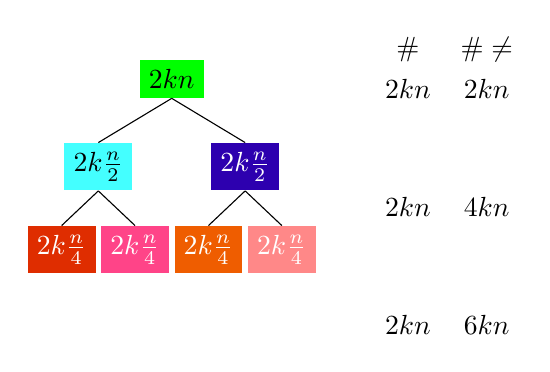
\begin{tikzpicture}
   \Tree
   [ .\node[fill=green]{$2kn$};    
       [.\node[fill=nodeblue1]{$2k\frac{n}{2}$};
           [.\node(n3l)[fill=nodered1, text=white]{$2k\frac{n}{4}$};]
           [.\node[fill=nodered2, text=white]{$2k\frac{n}{4}$};]
       ]
       [.\node[fill=nodeblue2, text=white]{$2k\frac{n}{2}$};
           [.\node[fill=nodered3, text=white]{$2k\frac{n}{4}$};]
           [.\node(n3r)[fill=nodered4, text=white]{$2k\frac{n}{4}$};]
       ]
   ]
   \node at (3,0.5) {$\#$};
   \node at (4,0.5) {$\# \neq$};
   \node at (3,0) {$2kn$};
   \node at (3,-1.5) {$2kn$};
   \node at (3,-3) {$2kn$};
   \node at (4,0) {$2kn$};
   \node at (4,-1.5) {$4kn$};
   \node at (4,-3) {$6kn$};
   \end{tikzpicture}
   }
   \caption{Bovenste drie niveaus}
   \label{fig:splitsingsvlakken-bsparbitrary-top}
\end{subfigure}
\begin{subfigure}[t]{0.64\textwidth}

    \resizebox{\textwidth}{!}{%
    \centering
     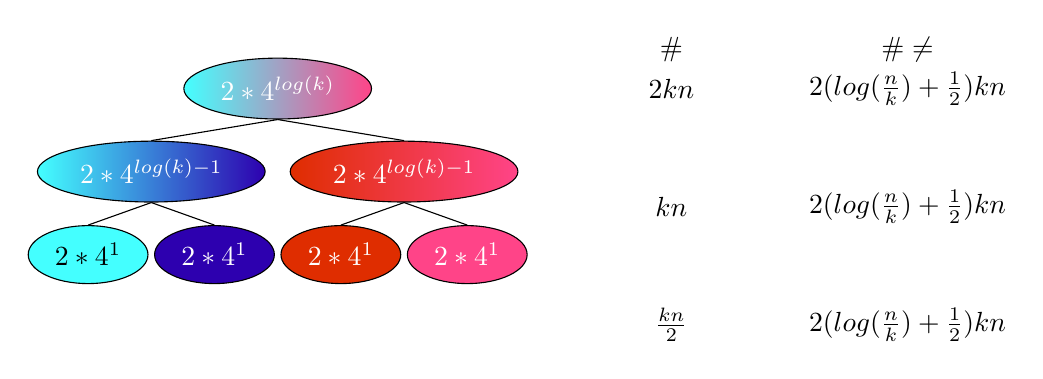
\begin{tikzpicture}
        \usetikzlibrary{arrows}
        \usetikzlibrary{shapes}
\tikzstyle{every tree node}=[draw, ellipse, align=center]
    \Tree
    [ .\node[shading = axis, left color=nodeblue1, right color=nodered2,shading angle=90, text=white]{$2*4^{log(k)}$};    
        [.\node[shading = axis, left color=nodeblue1, right color=nodeblue2,shading angle=90, text=white]{$2*4^{log(k) - 1}$};
            [.\node(n3l)[fill=nodeblue1, text=black]{$2*4^{1}$};]
            [.\node[fill=nodeblue2, text=white]{$2*4^{1}$};]
        ]
        [.\node[shading = axis, left color=nodered1, right color=nodered2,shading angle=90, text=white]{$2*4^{log(k) - 1}$};
            [.\node[fill=nodered1, text=white]{$2*4^{1}$};]
            [.\node(n3r)[fill=nodered2, text=white]{$2*4^{1}$};]
        ]
    ]
    \node at (5,0.5) {$\#$};
    \node at (8,0.5) {$\# \neq$};
    \node at (5,0) {$2kn$};
    \node at (5,-1.5) {$kn$};
    \node at (5,-3) {$\frac{kn}{2}$};
    \node at (8,0) {$2(log(\frac{n}{k}) + \frac{1}{2})kn$};
    \node at (8,-1.5) {$2(log(\frac{n}{k}) + \frac{1}{2})kn$};
    \node at (8,-3) {$2(log(\frac{n}{k}) + \frac{1}{2})kn$};
    \end{tikzpicture}
    }
    \caption{Onderste $log(k)$ niveaus}
    \label{fig:splitsingsvlakken-bsparbitrary-bottom}
 \end{subfigure}
   \caption[Splitsingsvlakken $\symBSParbitrary$ en $\symBSPcluster$]%
    {Splitsingsvlakken $\symBSParbitrary$ en $\symBSPcluster$ - \small Per niveau het aantal ($\#$) splitsingsvlakken en het totaal aantal verschillende ($\# \neq$) splitsingsvlakken gebruikt in bovenliggende niveaus bij de $\symBSParbitrary$ en $\symBSPcluster$ bomen.}
\end{figure}

    

    %Extra richtingen door random normalen te kiezen
    %Autopartitie van Ize maar gesweeped
    %Waarom zou dit werken ? : ...
    
\subsection{Geclusterde normalen}
    Bovenstaande $\symBSPsweep$ bomen bevatten een grote niet-deterministische factor.
    De $\symBSPcluster$ boom gebruikt het K-means clustering algoritme om deterministischere richtingen te bepalen.
    De normalen van de driehoeken in een knoop worden geclusterd in k clusters en de centra van deze clusters worden gebruikt als richtingen voor de $\symBSPsweep$ boom.
    Als er k of minder driehoeken in de knoop zitten, worden alle normalen als splitsingsrichting genomen, net zoals bij de $\symBSParbitrary$ boom.
    In tegenstelling tot de $\symBSParbitrary$ is het voor de $\symBSPcluster$ moeilijker om het totaal aantal mogelijke splitsingsvlakken te bepalen.
    In het algemeen kan elke clustering verschillende richtingen geven waardoor er oneindig veel mogelijke splitsingsrichtingen mogelijk zijn.
    De $\symBSPcluster$ boom is zeer gelijkaardig aan de $\symBSParbitrary$ boom waardoor het totaal aantal verschillende splitsingsvlakken die gebruikt worden, gelijk is. Analoog bestaan ook de $\symBSPclusterkd$ en $\symBSPclusterfastkd$ bomen.



    %TODO, identiek dezelfde afleidingen als arbitrary
    %Waarom zou dit werken ...

% TODO: vergelijking

\section{Vergelijking}
Tabel \ref{tab:boom-vergelijking-sweep} vergelijkt de hierboven besproken $\symBSPsweep$ bomen.
Alle drie bomen zijn algemene $\symBSP$ bomen die een convex veelvlak hebben als omhullend volume.
De $\symBSPsweep$ bomen zijn ontworpen om sweeping te ondersteunen en zo efficiënt de $SAH$ kosten te kunnen berekenen, zonder hulpstructuren.
De $\symBSPrandom$ boom is onafhankelijk van de lokale geometrie, de twee andere bomen bepalen hun splitsingsvlakken afhankelijk van de lokale geometrie.
De $\symBSPsweep$ bomen zijn makkelijk uit te breiden naar $\symBSPsweepfastkd$ bomen die de optimalisatie met de snelle $\symKd$ knoopdoorkruising gebruiken.
Per niveau gebruiken de $\symBSPsweep$ bomen niet altijd meer splitsingsvlakken dan de bestaande bomen, maar de $\symBSPsweep$ bomen gebruiken in totaal duidelijk meer verschillende splitsingsvlakken dan de bestaande bomen en zouden zich hierdoor beter moeten kunnen aanpassen aan complexe scenes.

\begin{table}[tb]
    \centering
    \begin{tabular}{@{}|l|c|c|c|@{}} \toprule      
            & $\symBSPrandom$     & $\symBSParbitrary$ & $\symBSPcluster$ \\ \midrule
      Omhullend volume & Convex veelvlak & Convex veelvlak & Convex veelvlak \\
      Sweeping                              &  Ja   & Ja & Ja    \\
      Geometrie afhankelijke vlakken & Nee & Ja & Ja \\
      Snelle Kd doorkruising                 & $\symBSPrandomfastkd$  & $\symBSParbitraryfastkd$  & $\symBSPclusterfastkd$    \\
      \# splitsingsvlakken per niveau       &  $2kn$   & $2kn$* & $2kn$*  \\
      totaal \# $\neq$ splitsingsvlakken           &  $2knlog(n)$   & $2(log(\frac{n}{k}) + \frac{1}{2})kn$ & $2(log(\frac{n}{k}) + \frac{1}{2})kn$     \\ \bottomrule
    \end{tabular}
    \caption[Vergelijking van de nieuwe soorten $\symBSP$ bomen.]{Vergelijking van de nieuwe soorten $\symBSP$ bomen - \small Deze tabel vat een aantal belangrijke eigenschappen van de nieuwe soorten $\symBSP$ bomen samen. *De onderste niveaus van $\symBSParbitrary$ en $\symBSPcluster$ bekijken minder dan $2kn$ splitsingsvlakken.}
    \label{tab:boom-vergelijking-sweep}
  \end{table}


%%% Local Variables: 
%%% mode: latex
%%% TeX-master: "masterproef"
%%% End: 
\chapter{Implementatie}
\label{hoofdstuk:implementatie}
In dit hoofdstuk wordt de implementatie van volgende $\symBSP$ bomen besproken: $\symKd$ boom, $\symRBSP$ boom, $\symRBSPKd$ boom, $\symBSPize$ boom, $\symBSPizefastkd$ boom, $\symBSPrandom$ boom, $\symBSPrandomkd$ boom, $\symBSPrandomfastkd$ boom, $\symBSParbitrary$ boom, $\symBSParbitrarykd$ boom, $\symBSParbitraryfastkd$ boom, $\symBSPcluster$ boom, $\symBSPclusterkd$ boom en $\symBSPclusterfastkd$ boom. \\

Het hoofdstuk start met een hoogniveau beschrijving (\ref{sec:h4-hoog-niveau}) van het algoritme om de boom te bouwen en het algoritme om de boom te intersecteren.
%Daarna wordt elk type boom besproken hoe hun knopen worden voorgesteld in het geheugen (\ref{sec:h4-voorstelling-knopen}.
%De specifieke implementaties van de bouwalgoritmes (\ref{sec:h4-bouwalgoritmes}) en intersectie-algoritmes (\ref{sec:h4-intersectie-algoritmes}) worden dan besproken.
%TODO

Uitbreiding pbrt-v3

%\section{Outline BSP-algoritmes}
%\section{Datastructuren knopen}
%\section{Bouwalgoritmes}
%    \subsection{SAH}
    %Intersectie willekeurig vlak & asgealigneerd
    % Snellere intersect / aangepast SAH
%\section{Intersectie-algoritmes}
\definecolor{codegreen}{rgb}{0,0.6,0}
\definecolor{codegray}{rgb}{0.5,0.5,0.5}
\definecolor{codepurple}{rgb}{0.58,0,0.82}
\definecolor{backcolor}{rgb}{0.95,0.95,0.92}
\lstdefinestyle{pseudoStyle}{
    backgroundcolor=\color{backcolor},   
    numberstyle=\tiny\color{codegray},
    stringstyle=\color{codepurple},
    %basicstyle=\footnotesize,
    breakatwhitespace=false,         
    breaklines=true,                 
    captionpos=b,                    
    keepspaces=true,                 
    numbers=left,                    
    numbersep=5pt,                  
    showspaces=false,                
    showstringspaces=false,
    showtabs=false,                  
    tabsize=2,
    basicstyle=\fontsize{9}{11}\selectfont\ttfamily
}
\lstset{style=pseudoStyle}

%TODO: slechteAanpassingen
\section{Hoog niveau beschrijving}
\label{sec:h4-hoog-niveau}
\subsection{Bouwalgoritme}
Het bouwalgoritme voor $\symBSP$ bomen heeft een aantal parameters:
\begin{itemize}
    \item $\symCost_\symIntersection$: De intersectiekost voor primitieven. Deze parameter is nodig voor de $\symSAH$ heuristiek.
    \item $\symCostTraversalKd$: De doorkruiskost voor $\symKd$ knopen. Deze parameter is nodig voor de $\symSAH$ heuristiek.
    \item $\symCostTraversalBSP$: De aparte doorkruiskost voor $\symBSP$ knopen. Deze parameter is nodig voor de $\symSAH$ heuristiek.
    \item $\symMaxPrims$: Elke knoop met $\symMaxPrims$ of minder primitieven wordt direct een bladknoop, er wordt niet geprobeerd om de knoop te splitsen.
    \item $\symMaxDepth$: De maximale diepte van de boom.
\end{itemize}
\begin{dutchalgorithm}
    \begin{algorithmic}
        \State $stack\gets \emptyset$
        \State Voeg een bouwknoop met alle primitieven toe aan de stack
        \While {$stack \neq \emptyset$}
            \State $b \gets $\Call{pop}{$stack$}
            \If {$b_{\symNbPrimitives} \leq \symMaxPrims$ \Or $b_{d} = \symMaxDepth$}
                \State \Call{maak\_blad\_knoop}{b}
                \State $continue$
            \EndIf
            \State $besteSplit \gets $ \Call{bepaal\_beste\_split}{b}
            \State $nietSplitKost \gets  b_{\symNbPrimitives}*\symCost_\symIntersection$
            \If {$besteSplit_{kost} > nietSplitKost$}
                \State $b_{slechteAanpassingen} \gets b_{slechteAanpassingen} + 1$
            \EndIf
            \If {$(besteSplit_{kost} > 4 * nietSplitKost$ \And $b_{\symNbPrimitives} < 16)$ \Or $besteSplit = None$ \Or $b_{slechteAanpassingen} = 3$}
                \State \Call{maak\_blad\_knoop}{b}
                \State $continue$
            \EndIf
            \State \Call{maak\_inwendige\_knoop}{b}
            \State Plaats de kindknopen als twee nieuwe bouwknopen op de stack
        \EndWhile
    \end{algorithmic}
    \caption{Bouwen van een BSP boom}
    \label{alg:bsp-bouw}
\end{dutchalgorithm}

Algoritme \ref{alg:bsp-bouw} toont de algemene vorm van het bouwalgoritme voor $\symBSP$ bomen.
Elk type $\symBSP$ boom wordt bepaald door de specifieke implementatie van de volgende functies:
\begin{enumerate}
    \item BEPAAL\_BESTE\_SPLIT(bouwknoop): Deze functie bepaalt de beste splitsing voor de knoop. Het resultaat bevat het splitsingsvlak en de bijhorende $\symSAH$ kost.
    \item MAAK\_BLAD\_KNOOP(bouwknoop): Deze functie maakt een bladknoop van de huidige bouwknoop.
    \item MAAK\_INWENDIGE\_KNOOP(bouwknoop): Deze functie maakt een inwendige knoop van de huidige bladknoop.
\end{enumerate}
De eerste functie omvat de specifieke eigenschappen van het type $\symBSP$ boom en bepaalt de kracht van dat type $\symBSP$ boom. 
Het resultaat van de tweede en derde functie is een specifieke representatie voor bladknopen / inwendige knopen die nuttig is voor het specifieke type $\symBSP$ boom.
In de volgende secties wordt bij elk type $\symBSP$ boom hun specifieke knooprepresentaties besproken.
De exacte implementaties van de functies om deze representaties in te vullen, zijn triviaal en worden niet expliciet beschreven.\\


Samengevat gaat Algoritme \ref{alg:bsp-bouw} voor elke knoop, die nog voldoende primitieven bevat en niet op de maximale diepte ligt, de beste splitsing bepalen en afhankelijk van de $\symSAH$ waarde bepalen of een splitsing moet gebeuren. 
Aangezien een slechte splitsing op een bepaald niveau, kan leiden tot een nuttige split op een lager niveau, wordt een knoop toch gesplitst als splitten nadelig is volgens de $\symSAH$ heuristiek.
Zulke \textit{slechte aanpassingen} worden niet gedaan als de kost van de beste split vier keer hoger is dan de kost om niet te splitsen en als er bovendien minder dan 16 primitieven in de knoop zitten.
Elk lusvrij pad van de wortelknoop naar elke andere knoop, mag maximaal twee zulke \textit{slechte aanpassingen} bevatten.
Dit komt neer op het feit dat een \textit{slechte aanpassing} enkel mag gebeuren als er minder dan twee voorouderknopen een \textit{slechte aanpassing} gedaan hebben.
Dit concept is overgenomen van de originele implementatie van de $\symKd$ boom in \textit{pbrt-v3}.

\subsection{Intersectie-algoritme}
Het intersectie-algoritme bepaalt het intersectiepunt tussen een straal en de $\symBSP$ boom.
Een straal wordt voorgesteld met de parametervoorstelling $\vec{s} = \vec{o} + t\vec{d}$.
Algoritme \ref{alg:bsp-intersectie} toont de algemene vorm van het intersectie-algoritme voor $\symBSP$ bomen.
Dit intersectie-algoritme is ontworpen voor zichtstralen en bepaalt dus het dichtste intersectiepunt.
De aanpassing naar een algoritme dat controleert of er een intersectiepunt bestaat, wat gebruikt kan worden voor schaduwstralen, is triviaal en wordt niet verder besproken.\\

\begin{dutchalgorithm}
    \begin{algorithmic}       
        \Function{intersecteer}{Boom b, Straal s}
            \State $geraakt_{omhullendVolume}, tMin, tMax \gets $ \Call{intersecteer}{$b_{omhullendVolume}$, s}
            \If {not $geraakt_{omhullendVolume}$}
                \State \Return false
            \EndIf
            \State $geraakt \gets false$
            \State $k \gets b_{wortelKnoop}$
            \State $stack\gets \emptyset$

            \While {$k \neq None$}
                \If {$s_{maxT} < tMin$}
                    \State $break$
                \EndIf
                \If {$k_{isInwendig}$}
                    \State $tVlak, linksEerst \gets$ \Call{doorkruis\_inwendige\_knoop}{k,s}
                    \If {$linksEerst$}
                        \State $k_1 \gets k_{linkerKind}$
                        \State $k_2 \gets k_{rechterKind}$
                    \Else
                        \State $k_1 \gets k_{rechterKind}$
                        \State $k_2 \gets k_{linkerKind}$
                    \EndIf
                    \If {$tVlak > tMax$ \Or $tVlak <= 0$}
                        \State $k \gets k_1$
                    \ElsIf {$tVlak < tMin$}
                        \State $k \gets k_2$
                    \Else
                        \State \Call{add}{$stack, \{k_2, tMin: tVlak, tMax: tMax\})$}
                        \State $k \gets k_1$
                        \State $tMax \gets tVlak$ 
                    \EndIf
                \Else
                    \If {\Call{intersecteer\_bladknoop}{k, s}}
                        \State $geraakt \gets true$
                    \EndIf
                    \If {$stack \neq \emptyset$}
                        \State $k, tMin, tMax \gets $\Call{pop}{$stack$}
                    \Else
                        \State $break$
                    \EndIf
                \EndIf
            \EndWhile
            \State \Return $geraakt$
        \EndFunction
    \end{algorithmic}
    \caption{Intersecteren van een BSP boom}
    \label{alg:bsp-intersectie}

\end{dutchalgorithm}  

Het algoritme maakt gebruik van de volgende functies:
\begin{enumerate}
    \item DOORKRUIS\_INWENDIGE\_KNOOP(knoop, straal): Deze functie bepaalt de intersectie van de gegeven straal met het splitsingsvlak van de gegeven inwendige knoop. Het resultaat bevat tVlak, de t waade waarvoor de straal intersecteert met het vlak en linksEerst, een boolean die aangeeft of de straal eerst door de linkerkindknoop gaat of niet.
    \item INTERSECTEER\_BLAD\_KNOOP(knoop, straal): Deze functie bepaalt de intersectie van de primitieven in de gegeven bladknoop met de gegeven straal.     
    \item INTERSECTEER(volume, straal): Deze functie bepaalt de intersectie van het omhullend volume van de boom en de straal. Het resultaat bevat een booleaans waarde, die aanduidt of het volume geraakt wordt door de straal. Als het volume geraakt wordt, bevat het ook de waarde tMin, de t waarde waarvoor de straal het volume binnengaan, en tMax, de t waarde waarvoor de straal het volume verlaat.
\end{enumerate}

De eerste functie is afhankelijk van de specifieke representatie voor bladknopen / inwendige knopen die gebruikt worden voor het specifieke type $\symBSP$ boom.
Bij de bespreking van de knooprepresentaties in de volgende secties, wordt steeds de implementatie van deze functie voor die knooprepresentatie getoond.
De tweede functie is hetzelfde voor alle knopen die besproken worden, elke driehoek in de bladknoop wordt op intersectie met de straal getest.
De derde functie bepaalt de intersectie van het omhullende volume van de $\symBSP$ boom met de straal. 
Bij alle besproken bomen wordt dit voorgesteld door een asgealigneerde balk.
Intersectie berekenen met een asgealigneerde balk is triviaal.

\section{$\symKd$ boom}
\label{sec:h4-kd}

De implementatie van de $\symKd$ boom is gebasseerd op de $\symKd$ boom implementatie van pbrt.
De $\symKd$ boom maakt gebruik van $\symKd$ knopen. 
Tabel \ref{tab:voorstelling-kd-knoop} toont de representatie van zowel inwendige $\symKd$ knopen als blad $\symKd$ knopen. 
Zowel inwendige knopen als bladknopen worden voorgesteld met 64 bits en bevatten de \textit{flags} variabele.
Als de \textit{flags} variabele gelijk is aan 3, is het een bladknoop.
Bij inwendige knopen stelt die variabele de as voor waarlangs gesplitst wordt: 0 is x, 1 is y en 2 is z.\\

De inwendige knopen bevatten extra informatie over hun splitsingsvlak via \textit{tSplit}.
Deze \textit{tSplit} variabele bepaalt de locatie van het vlak langs de as.
De knopen van een boom worden opgeslagen in een lijst, bij een inwendige knoop wordt zijn linkerkindknoop opgeslagen op de volgende index in de lijst.
De index van de rechterkindknoop, wordt opgeslagen in de \textit{tweedeKindIndex} variabele.\\

De bladknopen bevatten informatie over hun primitieven via \textit{n} en \textit{primitiefOffset}.
De \textit{n} variabele stelt het aantal primitieven in de bladknoop voor.
De \textit{primitiefOffset} variabele verwijst naar de primitieven in de bladknoop.
Als er maar één primitief in de knoop zit, wijst de variabele rechtstreeks naar het primitief.
Als er meerdere primitieven in de knoop zitten, stelt het in index voor in een lijst.
Elk element in die lijst met een index tussen \textit{primitiefOffset} en $\textit{primitiefOffset} + \textit{n}$ wijst dan naar een primitief in de bladknoop.\\

\begin{table}
    \centering
    \begin{tabular}{@{}|c|c|c|c|@{}} \toprule      
    Inwendig & bits & Blad & bits \\ \midrule
    tSplit & 32 & primitief Offset & 32 \\
    flags  & 2  &  flags   & 2    \\
    tweedeKindIndex & 30 & $\symNbPrimitives$ & 30 \\ \hline \hline
    & 64 & & 64    \\ \bottomrule
    \end{tabular}
    \caption[Voorstelling $\symKd$ knoop]{Voorstelling $\symKd$ knoop - \small }
    \label{tab:voorstelling-kd-knoop}
\end{table}            
\begin{dutchalgorithm}
    \begin{algorithmic}       
        \Function{doorkruis\_inwendige\_knoop}{$\symKd$ Knoop k, Straal s}
            \State $as <- k_{splitsAs}$
            \State $tVlak \gets $ \Call{kd\_vlak\_afstand}{$k_{splitPos}$, s, $\frac{1}{\vec{s_d}}$, as}
            \State $linksEerst \gets \vec{s_o}[as] < k_{splitPos}$ \Or $(\vec{s_o}[as] = k_{splitPos}$ \And $s_d[as] \leq 0)$
            \State \Return $tVlak$, $linksEerst$
        \EndFunction
    \end{algorithmic}
    \caption{Doorkruisen van een inwendige $\symKd$ knoop.}
    \label{alg:kd-inwendige-doorkruising}
\end{dutchalgorithm}
\begin{dutchalgorithm}
    \begin{algorithmic}       
        \Function{kd\_vlak\_afstand}{splitPositie, s, inverseRichting, as}
            \State \Return $(splitPos - \vec{s_o}[as]) * \vec{inverseRichting}[as]$
        \EndFunction
    \end{algorithmic}
    \caption{Intersectie tussen een asgealigneerd vlak en een straal.}
    \label{alg:kd-vlak-intersectie}
\end{dutchalgorithm}
Algoritme \ref{alg:kd-inwendige-doorkruising} toont het algoritme om inwendige $\symKd$ knopen te doorkruisen.
Het gebruikt de functie KD\_VLAK\_INTERSECTIE (algoritme \ref{alg:kd-vlak-intersectie}) om te intersecteren met een asgealigneerd vlak.
De inverse van de richting van de straal ($\frac{1}{\vec{s_d}}$) moet voor elke straal slechts één keer berekend worden.

%TODO: beste split algo
\begin{dutchalgorithm}
    \begin{algorithmic}       
        \Function{bepaal\_beste\_split}{bouwKnoop}
            \State $besteAs$, $besteT$ $\gets None$, $None$
            \State $besteKost$, $oudeKost$ $\gets \infty$, $\symCost_\symIntersection * bouwknoop_n$
            \For{$as \in \{0, 1, 2\}$}
                \State $\forall i: randen[2i]\gets$ \Call{linkerrand}{$b_{primitieven}[i]$, as}
                \State $\forall i: randen[2i+1]\gets$ \Call{rechterrand}{$b_{primitieven}[i]$, as}
                \State \Call{sorteer}{randen}
                \State $n_{links}, n_{rechts} \gets 0, bouwknoop_n$
                \For{$rand \in randen$}
                    \If{$rand_{isRechts}$}
                        \State $n_{rechts} \gets n_{rechts} - 1$
                    \EndIf
                    \State $kost \gets$ \Call{SAH}{$\symCostTraversal$,$\symCost_\symIntersection$,$\symSA_{links}$,
                    $\symSA_{rechts}$,
                    $n_{links}$, $n_{rechts}$}
                    \If{$kost < besteKost$}
                        \State $besteKost, besteAs, besteT \gets kost, as, rand_t$
                    \EndIf
                    \If{$rand_{isLinks}$}
                        \State $n_{links} \gets n_{links} + 1$
                    \EndIf
                \EndFor                
            \EndFor
            \State \Return $(splitPos - \vec{s_o}[as]) * \vec{inverseRichting}[as]$
        \EndFunction
    \end{algorithmic}
    \caption{Beste split voor een bouwknoop b bij een $\symKd$ boom.}
    \label{alg:kd-beste-split}
\end{dutchalgorithm}



\section{$\symRBSP$ boom}
\label{sec:h4-rbsp}
Implementatie gebasseerd op 
De $\symRBSP$ boom maakt gebruik van $\symRBSP$ knopen. 
Tabel \ref{tab:voorstelling-rbsp-knoop} toont de representatie van zowel inwendige $\symRBSP$ knopen als blad $\symRBSP$ knopen.
\begin{table}
        \centering
        \begin{tabular}{@{}|c|c|c|c|@{}} \toprule      
        Inwendig & bits & Blad & bits \\ \midrule
        tSplit & 32 & primitief Offset & 32 \\
        flags  & $log_2(k + 1)$  &  flags   & $log_2(k + 1)$   \\
        tweedeKindIndex & 32 - $log_2(k + 1)$ & $\symNbPrimitives$ & 32 - $log_2(k + 1)$ \\ \hline \hline
        & 64 & & 64    \\ \bottomrule
        \end{tabular}
    \caption[Voorstelling $\symRBSP$ knoop]{Voorstelling $\symRBSP$ knoop - \small }
    \label{tab:voorstelling-rbsp-knoop}    
\end{table}   

\begin{dutchalgorithm}
    \begin{algorithmic}       
        \Function{vlak\_afstand}{$\vec{normaal}$, splitPositie, s}
            \State $projOorsprong \gets \vec{normaal} \cdot \vec{s_o}$
            \State $invProjRichting \gets \frac{1}{\vec{normaal} \cdot \vec{s_d}}$
            \State $afstand \gets (splitPos - projOorsprong) * invProjRichting $
            \State \Return projOorsprong, invProjRichting, afstand
        \EndFunction
    \end{algorithmic}
    \caption{Intersectie tussen een vlak en een straal.}
\end{dutchalgorithm}

\begin{dutchalgorithm}
    \begin{algorithmic}       
        \Function{doorkruis\_inwendige\_knoop}{$\symRBSP$ Knoop k, Straal s}
            \State $richtingId \gets k_{splitsAs}$
            \State $tVlak, projOorsprong, invProjRichting \gets $ \Call{vlak\_afstand}{$\vec{richtingen[richtingId]}$, $k_{splitPos}$, s}
            \State $linksEerst \gets projOorsprong < k_{splitPos}$ \Or $(projOorsprong = k_{splitPos}$ \And $invProjRichting \leq 0)$
            \State \Return $tVlak$, $linksEerst$
        \EndFunction
    \end{algorithmic}
    \caption{Doorkruisen van een inwendige $\symRBSP$ knoop.}
\end{dutchalgorithm}

\section{$\symRBSPKd$ boom}
\label{sec:h4-rbspkd}
Nieuwe implementatie, uitbreiding $\symRBSP$ met de snelle $\symKd$ doorkruistechniek van \authorIze{}.
$\symRBSPKd$ knoop identiek aan $\symRBSP$ knoop in termen van voorstelling, andere intersectie

\begin{dutchalgorithm}
    \begin{algorithmic}       
        \Function{doorkruis\_inwendige\_knoop}{$\symRBSPKd$ Knoop k, Straal s}
            \State $richtingId \gets k_{splitsAs}$
            \If {$richtingId < 3$}
                \State $tVlak \gets $ \Call{kd\_vlak\_afstand}{$k_{splitPos}$, s, $\frac{1}{\vec{s_d}}$, richtingId}
                \State $linksEerst \gets \vec{s_o}[richtingId] < k_{splitPos}$ \Or $(\vec{s_o}[richtingId] = k_{splitPos}$ \And $s_d[richtingId] \leq 0)$
                \State \Return $tVlak$, $linksEerst$
            \Else
                \State $tVlak, projOorsprong, invProjRichting \gets $ \Call{vlak\_afstand}{$\vec{richtingen[richtingId]}$, $k_{splitPos}$, s}
                 \State $linksEerst \gets projOorsprong < k_{splitPos}$ \Or $(projOorsprong = k_{splitPos}$ \And $invProjRichting \leq 0)$
                \State \Return $tVlak$, $linksEerst$
            \EndIf
        \EndFunction
    \end{algorithmic}
    \caption{Doorkruisen van een inwendige $\symRBSPKd$ knoop.}
\end{dutchalgorithm}

\section{$\symBSPize$ boom}
\label{sec:h4-bspize}
Vergelijk representatie met die van de paper
\begin{table}
        \centering
        \begin{tabular}{@{}|c|c|c|c|@{}} \toprule      
            Inwendig & bits & Blad & bits \\ \midrule
            tSplit & 32 & primitief Offset & 32 \\
            flags  & 1  &  flags   & 1    \\
            tweedeKindIndex & 31 & $\symNbPrimitives$ & 31 \\
            splitRichting & 96 &  &  \\ \hline \hline
            & 160 & & 64    \\ \bottomrule
        \end{tabular}
    \caption[Voorstelling $\symBSP$ knoop]{Voorstelling $\symBSP$ knoop - \small }
    \label{tab:voorstelling-bsp-knoop}
\end{table}   

  
\begin{dutchalgorithm}
    \begin{algorithmic}       
        \Function{doorkruis\_inwendige\_knoop}{$\symBSP$ Knoop k, Straal s}
            \State $tVlak, projOorsprong, invProjRichting \gets $ \Call{vlak\_afstand}{$\vec{k_{splitsRichting}}$, $k_{splitPos}$, s}
            \State $linksEerst \gets projOorsprong < k_{splitPos}$ \Or $(projOorsprong = k_{splitPos}$ \And $invProjRichting \leq 0)$
            \State \Return $tVlak$, $linksEerst$
        \EndFunction
    \end{algorithmic}
    \caption{Doorkruisen van een inwendige $\symBSP$ knoop.}
\end{dutchalgorithm}

\section{$\symBSPizefastkd$ boom}
\label{sec:h4-bspizefastkd}
\begin{table}
        \centering
        \begin{tabular}{@{}|c|c|c|c|@{}} \toprule      
            Inwendig & bits & Blad & bits \\ \midrule
            tSplit & 32 & primitief Offset & 32 \\
            flags  & 3  &  flags   & 3   \\
            tweedeKindIndex & 29 & $\symNbPrimitives$ & 29 \\
            splitRichting & 96 &  &  \\ \hline \hline
            & 160 & & 64    \\ \bottomrule
        \end{tabular}
    \caption[Voorstelling $\symBSPKd$ knoop]{Voorstelling $\symBSPKd$ knoop - \small }
    \label{tab:voorstelling-bspkd-knoop}
\end{table}   


\begin{dutchalgorithm}
    \begin{algorithmic}       
        \Function{doorkruis\_inwendige\_knoop}{$\symBSPKd$ Knoop k, Straal s}
            \State $isKdKnoop \gets k_{flags} < 4$
            \If {$isKdKnoop$}
                \State $as \gets k_{flags}$
                \State $tVlak \gets $ \Call{kd\_vlak\_afstand}{$k_{splitPos}$, s, $\frac{1}{\vec{s_d}}$, as}
                \State $linksEerst \gets \vec{s_o}[as] < k_{splitPos}$ \Or $(\vec{s_o}[as] = k_{splitPos}$ \And $s_d[as] \leq 0)$
                \State \Return $tVlak$, $linksEerst$
            \Else
                \State $tVlak, projOorsprong, invProjRichting \gets $ \Call{vlak\_afstand}{$\vec{k_{splitsRichting}}$, $k_{splitPos}$, s}
                 \State $linksEerst \gets projOorsprong < k_{splitPos}$ \Or $(projOorsprong = k_{splitPos}$ \And $invProjRichting \leq 0)$
                \State \Return $tVlak$, $linksEerst$
            \EndIf
        \EndFunction
    \end{algorithmic}
    \caption{Doorkruisen van een inwendige $\symBSPKd$ knoop.}
\end{dutchalgorithm}

\section{$\symBSPsweep$ boom}
\label{sec:h4-bspsweep}
Intersectie identiek aan andere, zelfde soorten knopen.

\paragraph{Selectie beste splitsingsvlak}
Algoritme $\symBSPsweep$ en $\symBSPsweep +$ hetzelfde, behalve de $getDirections$
Apart voor $\symBSPsweepkd$


\begin{table}
    \centering
    \begin{tabular}{@{}|c|c|@{}} \toprule      
    $\symBSP$ boom & Knooptype \\ \midrule
    $\symKd$ & $\symKd$ \\
    $\symRBSP$ & $\symRBSP$  \\
    $\symRBSPKd$ & $\symRBSPKd$  \\
    $\symBSPize$ &  $\symBSP$ \\
    $\symBSPizefastkd$ & $\symBSPKd$ \\
    $\symBSPsweepmaybewithkd$ & $\symBSP$ \\
    $\symBSPsweepkd$ & $\symBSPKd$ \\ \bottomrule
    \end{tabular}
    \caption[Gebruikte soorten knopen voor alle soorten $\symBSP$ bomen]{Gebruikte soorten knopen voor alle soorten $\symBSP$ bomen - \small}
    \label{tab:voorstelling-knoop-boom}
\end{table}

%
%\section{$\symKd$ boom}
%\section{$\symRBSP$ boom}
%\section{$\symBSPize$}
%\section{$\symBSPsweep$}
%\subsection{Algemeen}
%\subsection{$\symBSPrandom$}
%\subsection{$\symBSParbitrary$}
%\subsection{$\symBSPcluster$}


%%% Local Variables: 
%%% mode: latex
%%% TeX-master: "masterproef"
%%% End: 
\newcommand\skipCaption[1]{
  \vspace*{-6mm}
  \caption{#1}
}

\newcommand\skipCaptionA[2]{
  \vspace*{-#1mm}
  \caption{#2}
}

\chapter{Resultaten}
\label{hoofdstuk:resultaten}
Dit hoofdstuk bespreekt de resultaten van de nieuwe $\symBSPsweep$ bomen.
In sectie \ref{h5:praktische-aspecten} worden een aantal praktische aspecten omtrent de testopstelling besproken zoals de scenes, de gebruikte parameters en het gebruikte computersysteem.
Daarna bespreken we de invloed van het aantal richtingen op de vorm (sectie \ref{h5-richtingen-bespreking}) en kwaliteit (sectie \ref{h5-richtingen-kwaliteit}) van de negen soorten $\symBSPsweep$ bomen.
De laatste sectie (sectie \ref{h5-vergelijken}) vergelijkt de beste $\symBSPsweep$ bomen met de bomen besproken in hoofdstuk \ref{hoofdstuk:voorgaand-werk}.

\section{Praktische aspecten}
\label{h5:praktische-aspecten}
Alle $\symBSP$ bomen zijn geïmplementeerd in het pbrt framework zoals besproken in hoofdstuk \ref{hoofdstuk:implementatie}. 
Dit framework maakt geen gebruik van optimalisaties zoals SIMD instructies en de GPU. 
Hierdoor kan de kracht van de verschillende bomen objectief vergeleken worden.\\

Figuur \ref{fig:results-scenes} toont de gebruikte testscenes en tabel \ref{tab:results-statistics-scenes} toont informatie over deze scenes.
De Killeroo Been scene is een scene waarbij algemene $\symBSP$ bomen voordeel hebben ten opzichte van de $\symKd$ boom omwille van de complexe geometrie waarop is ingezoomd.
De drie andere scenes zijn realistische indoor scenes.
Alle scenes maken gebruik van Halton sampling met een specifiek aantal stralen per pixel \textit{spp}.
De globale belichting wordt berekend via \textit{path tracing} waarbij steeds een maximale diepte van 5 gebruikt wordt, behalve bij de museum scene waar enkel directe belichting gebruikt wordt.\\

\begin{figure}
  \begin{subfigure}[t]{0.25\textwidth}
    \centering
    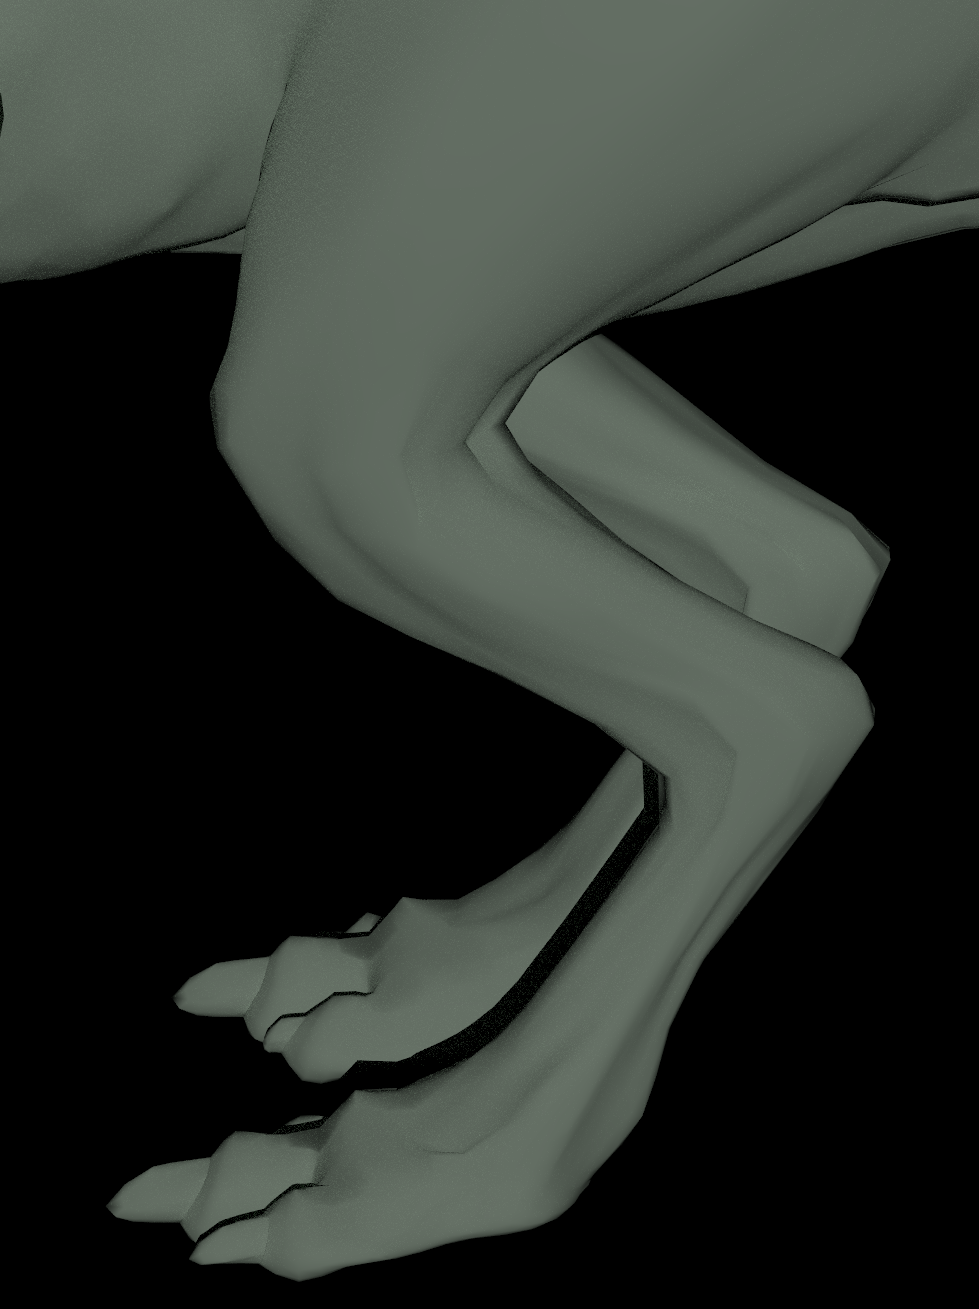
\includegraphics[width=0.6\linewidth]{img/killerooFeet}
    \caption{Killeroo Been scene}
    \label{fig:results-scene-killeroo-been}    
  \end{subfigure}
  \begin{subfigure}[t]{0.20\textwidth}
    \centering
    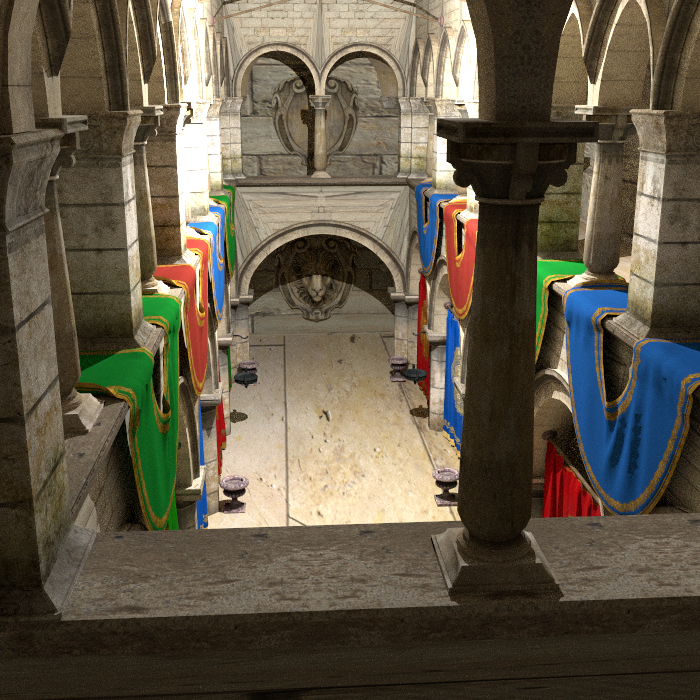
\includegraphics[width=1\linewidth]{img/sponza}
    \caption{Sponza scene}
    \label{fig:results-scene-sponza}    
  \end{subfigure}
  \begin{subfigure}[t]{0.29\textwidth}
    \centering
    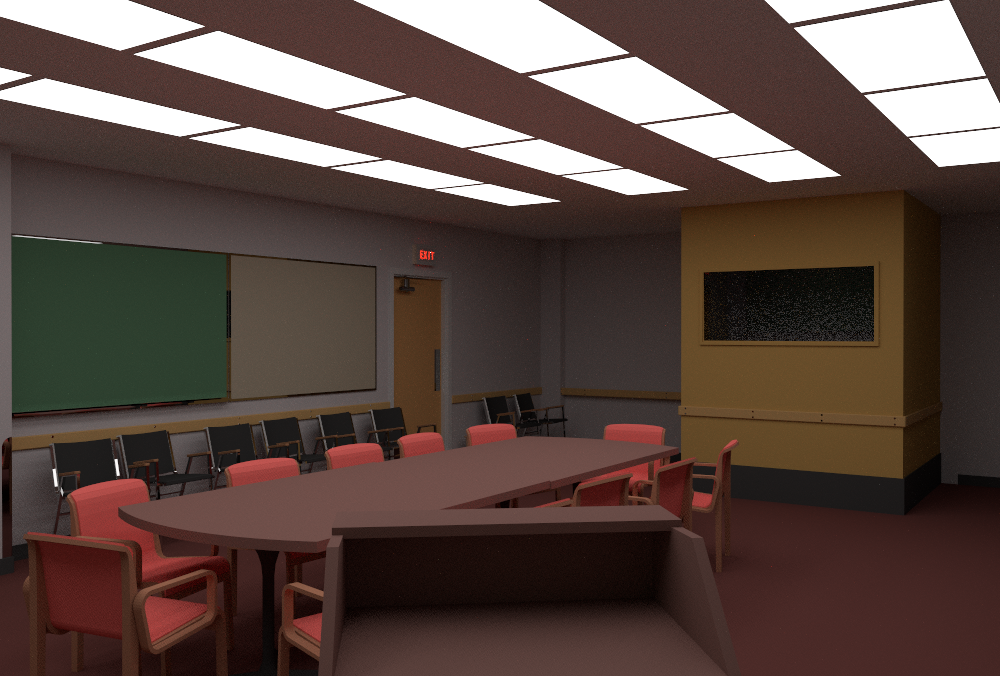
\includegraphics[width=1\linewidth]{img/conferencehall}
    \caption{Conference scene}
    \label{fig:results-scene-conference}    
  \end{subfigure}
  \begin{subfigure}[t]{0.20\textwidth}
    \centering
    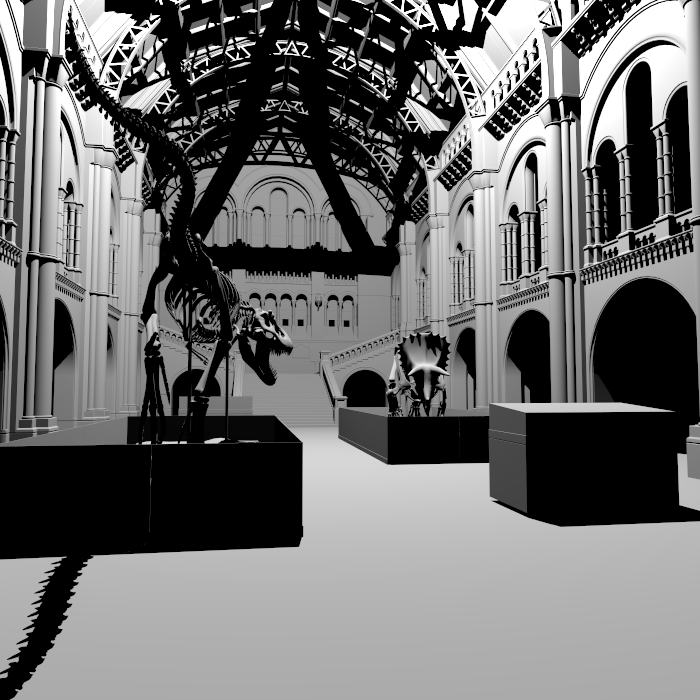
\includegraphics[width=1\linewidth]{img/museum}
    \caption{Museum scene}
    \label{fig:results-scene-museum}    
  \end{subfigure}
  \caption[Testscenes]{Testscenes - \small De testscenes gebruikt om de nieuwe $\symBSP$ te testen}
  \label{fig:results-scenes}
\end{figure}

\begin{table}
  \centering
  \begin{tabular}{@{}lcccc@{}} \toprule
  Scene & Aantal driehoeken & Resolutie & Sampling per pixel & Belichting\\ \midrule
  Killeroo Been & 33264 & 5000x5000 & Halton, 8spp & \textit{path tracing}, diepte 5\\
  Sponza & 227309 & 700x700 & Halton, 64spp & \textit{path tracing}, diepte 5\\
  Conference & 123651 & 1000x676 & Halton, 64spp & \textit{path tracing}, diepte 5\\
  Museum & 1462840 & 700X700 & Halton, 64spp & \textit{path tracing}, diepte 1\\ \bottomrule
 \end{tabular}
  \caption[Statistieken Testscenes]{Statistieken Testscenes - \small Statistieken van de testscenes gebruikt om de nieuwe $\symBSP$ te testen}
  \label{tab:results-statistics-scenes}
\end{table}

Tabel \ref{tab:results-parameters} toont de parameterwaarden die gebruikt zijn bij de testen. De formule voor de maximale diepte is afhankelijk van het aantal driehoeken n en is bedacht door \authorHavranBittner{} \cite{havran2002improving} voor $\symKd$ bomen. Deze parameterwaarden zijn niet geoptimaliseerd en kunnen mogelijks beter worden afgesteld.
De specificaties van het gebruikte computersysteem worden getoond in figuur \ref{tab:results-specs}.
\begin{table}
  \centering
  \begin{tabular}{@{}lc@{}} \toprule
  Parameter & Waarde \\ \midrule
  $\symCost_\symIntersection$ & 80 \\
  $\symCostTraversalKd$ & 1 \\
  $\symCostTraversalBSP$ & 5 \\
  $\symMaxPrims$ & 1 \\
  $\symMaxDepth$ & $k1log_2(n) + k2$ met $k1 = 1.6$ en $k2 = 2$ \\
  \bottomrule
 \end{tabular}
  \caption[Gebruikte parameterwaarden]{Gebruikte parameterwaarden - \small De waarden voor de parameters gebruikt om de nieuwe $\symBSP$ te testen}
  \label{tab:results-parameters}
\end{table}

\begin{table}
  \centering
  \begin{tabular}{@{}lc@{}} \toprule
  Parameter & Waarde \\ \midrule
  CPU & Intel Core i7-6700HQ CPU @ 2.60GHz x 8 \\
  Geheugen & 16 GB DDR4 \\
  Besturingssysteem & Ubuntu 18.04.2 LTS 64-bit \\
  \bottomrule
 \end{tabular}
  \caption[Specificaties computersysteem]{Specificaties computersysteem - \small De specificaties van het gebruikte computersysteem.}
  \label{tab:results-specs}
\end{table}

\newcommand{\plotVsK}[5] {
  \begin{tikzpicture}[scale=0.5]
    \begin{axis}[
      axis lines = left,
      ylabel = #5,
      xlabel = K,
      ymin=#3, ymax=#4,
      xmin=2,
      width=1.8\textwidth,
      height=2.2\textwidth,
      cycle multi list={%
        color list\nextlist
        [3 of]mark list
      },
      legend style={at={(0.5,-0.15)}, anchor=north,legend columns=3},
      title = #2,
  ]
    \addplot table [x=K, y=#1, col sep=comma] {data/bsprandomRender.csv};
    \addlegendentry{$\symBSPrandom$}
    \addplot table [x=K, y=#1, col sep=comma] {data/bsprandomwithkdRender.csv};
    \addlegendentry{$\symBSPrandomkd$}
    \addplot table [x=K, y=#1, col sep=comma] {data/bsprandomfastkdRender.csv};
    \addlegendentry{$\symBSPrandomfastkd$}
    
    \addplot table [x=K, y=#1, col sep=comma] {data/bsparbitraryRender.csv};
    \addlegendentry{$\symBSParbitrary$}
    \addplot table [x=K, y=#1, col sep=comma] {data/bsparbitrarywithkdRender.csv};
    \addlegendentry{$\symBSParbitrarykd$}
    \addplot table [x=K, y=#1, col sep=comma] {data/bsparbitraryfastkdRender.csv};
    \addlegendentry{$\symBSParbitraryfastkd$}
    
    \addplot table [x=K, y=#1, col sep=comma] {data/bspclusterRender.csv};
    \addlegendentry{$\symBSPcluster$}
    \addplot table [x=K, y=#1, col sep=comma] {data/bspclusterwithkdRender.csv};
    \addlegendentry{$\symBSPclusterkd$}
    \addplot table [x=K, y=#1, col sep=comma] {data/bspclusterfastkdRender.csv};
    \addlegendentry{$\symBSPclusterfastkd$}
      \end{axis}
    \end{tikzpicture}
}

\newcommand{\plotFastKdVsK}[5] {
  \begin{tikzpicture}[scale=0.5]
    \begin{axis}[
      axis lines = left,
      ylabel = #5,
      xlabel = K,
      ymin=#3, ymax=#4,
      width=1.8\textwidth,
      height=2.2\textwidth,
      cycle multi list={%
        color list\nextlist
        mark=triangle*
      },
      legend style={at={(0.5,-0.15)}, anchor=north,legend columns=3},
      title = #2,
  ]
    
    \addplot table [x=K, y=#1, col sep=comma, mark=diamond*] {data/bsprandomfastkdRender.csv};
    \addlegendentry{$\symBSPrandomfastkd$}
    
    \addplot table [x=K, y=#1, col sep=comma, mark=diamond*] {data/bsparbitraryfastkdRender.csv};
    \addlegendentry{$\symBSParbitraryfastkd$}
    
    \addplot table [x=K, y=#1, col sep=comma, mark=diamond*] {data/bspclusterfastkdRender.csv};
    \addlegendentry{$\symBSPclusterfastkd$}
      \end{axis}
    \end{tikzpicture}
}

\newcommand{\plotRendertimeKScenes}[4] {
  \begin{tikzpicture}
    \begin{axis}[
      axis lines = left,
      ylabel = Procentuele tijd tov de $\symKd$ boom,
      xlabel = K,
      ymin=#3, ymax=#4,
      width=0.5\textwidth,
      height=0.8\textwidth,
      %cycle multi list={%
      %  color list\nextlist
      %  [3 of]mark list
      %},
      title = #2,
      legend pos=north east,
  ]
    \addplot table [x=K, y=RendertimeTovKdFeet, col sep=comma] {#1};
    \addlegendentry{Med Killeroo Been}
    \addplot table [x=K, y=RendertimeTovKdSponza, col sep=comma] {#1};
    \addlegendentry{Med Sponza Been}
    \addplot table [x=K, y=RendertimeTovKdConference, col sep=comma] {#1};
    \addlegendentry{Med Conference Been}
    
      \end{axis}
    \end{tikzpicture}
}
\newcommand{\plotSAKScenes}[4] {
  \begin{tikzpicture}
    \begin{axis}[
      axis lines = left,
      ylabel = Procentuele SA tov de $\symKd$ boom,
      xlabel = K,
      ymin=#3, ymax=#4,
      width=0.5\textwidth,
      height=0.8\textwidth,
      %cycle multi list={%
      %  color list\nextlist
      %  [3 of]mark list
      %},
      title = #2,
      legend pos=north east,
  ]
    \addplot table [x=K, y=SATovKdFeet, col sep=comma] {#1};
    \addlegendentry{Killeroo Been}
    \addplot table [x=K, y=SATovKdSponza, col sep=comma] {#1};
    \addlegendentry{Sponza Been}
    \addplot table [x=K, y=SATovKdConference, col sep=comma] {#1};
    \addlegendentry{Conference Been}
    
      \end{axis}
    \end{tikzpicture}
}
\newcommand{\plotPrimIntBothKScenes}[4] {
  \begin{tikzpicture}
    \begin{axis}[
      axis lines = left,
      ylabel = Procentueel aantal intersecties tov de $\symKd$ boom,
      xlabel = K,
      ymin=#3, ymax=#4,
      width=0.5\textwidth,
      height=0.8\textwidth,
      cycle multi list={%
        color list\nextlist
        [2 of]mark list
      },
      title = #2,
      legend pos=north east,
  ]
    \addplot table [x=K, y=nbPrimIntTovKdFeet, col sep=comma] {#1};
    \addlegendentry{Prim Killeroo Been}    
    \addplot table [x=K, y=nbPrimIntPTovKdFeet, col sep=comma] {#1};
    \addlegendentry{Sec Killeroo Been}
    
    \addplot table [x=K, y=nbPrimIntTovKdSponza, col sep=comma] {#1};
    \addlegendentry{Prim Sponza Been}    
    \addplot table [x=K, y=nbPrimIntPTovKdSponza, col sep=comma] {#1};
    \addlegendentry{Sec Sponza Been}
    
    \addplot table [x=K, y=nbPrimIntTovKdConference, col sep=comma] {#1};
    \addlegendentry{Prim Conference Been}
    \addplot table [x=K, y=nbPrimIntPTovKdConference, col sep=comma] {#1};
    \addlegendentry{Sec Conference Been}
    
      \end{axis}
    \end{tikzpicture}
}
\newcommand{\plotTravBothKScenes}[4] {
  \begin{tikzpicture}
    \begin{axis}[
      axis lines = left,
      ylabel = Procentueel aantal doorkruisingen tov de $\symKd$ boom,
      xlabel = K,
      ymin=#3, ymax=#4,
      width=0.5\textwidth,
      height=0.8\textwidth,
      cycle multi list={%
        color list\nextlist
        [2 of]mark list
      },
      title = #2,
      legend pos=outer north east,
  ]
    \addplot table [x=K, y=nbNodeTravTovKdFeet, col sep=comma] {#1};
    \addlegendentry{Prim Killeroo Been}    
    \addplot table [x=K, y=nbNodeTravPTovKdFeet, col sep=comma] {#1};
    \addlegendentry{Sec Killeroo Been}
    
    \addplot table [x=K, y=nbNodeTravTovKdSponza, col sep=comma] {#1};
    \addlegendentry{Prim Sponza Been}    
    \addplot table [x=K, y=nbNodeTravPTovKdSponza, col sep=comma] {#1};
    \addlegendentry{Sec Sponza Been}
    
    \addplot table [x=K, y=nbNodeTravTovKdConference, col sep=comma] {#1};
    \addlegendentry{Prim Conference Been}
    \addplot table [x=K, y=nbNodeTravPTovKdConference, col sep=comma] {#1};
    \addlegendentry{Sec Conference Been}
    
      \end{axis}
    \end{tikzpicture}
}
\newcommand{\plotKdTravProcBothKScenes}[4] {
  \begin{tikzpicture}
    \begin{axis}[
      axis lines = left,
      ylabel = Procentueel aantal $\symKd$ doorkruisingen,
      xlabel = K,
      ymin=#3, ymax=#4,
      width=0.5\textwidth,
      height=0.8\textwidth,
      cycle multi list={%
        color list\nextlist
        [2 of]mark list
      },
      title = #2,
      legend pos=outer north east,
  ]
    \addplot table [x=K, y=nbKdNodeTravPercFeet, col sep=comma] {#1};
    \addlegendentry{Prim Killeroo Been}    
    \addplot table [x=K, y=nbKdNodeTravPPercFeet, col sep=comma] {#1};
    \addlegendentry{Sec Killeroo Been}
    
    \addplot table [x=K, y=nbKdNodeTravPercSponza, col sep=comma] {#1};
    \addlegendentry{Prim Sponza Been}    
    \addplot table [x=K, y=nbKdNodeTravPPercSponza, col sep=comma] {#1};
    \addlegendentry{Sec Sponza Been}
    
    \addplot table [x=K, y=nbKdNodeTravPercConference, col sep=comma] {#1};
    \addlegendentry{Prim Conference Been}
    \addplot table [x=K, y=nbKdNodeTravPPercConference, col sep=comma] {#1};
    \addlegendentry{Sec Conference Been}
    
      \end{axis}
    \end{tikzpicture}
}
\newcommand{\plotKdNodeProcBothKScenes}[4] {
  \begin{tikzpicture}
    \begin{axis}[
      axis lines = left,
      ylabel = Procentueel aantal $\symKd$ knopen,
      xlabel = K,
      ymin=#3, ymax=#4,
      width=0.5\textwidth,
      height=0.8\textwidth,
      cycle multi list={%
        color list\nextlist
        [1 of]mark list
      },
      title = #2,
      legend pos=outer north east,
  ]
    \addplot table [x=K, y=nbKdNodePercFeet, col sep=comma] {#1};
    \addlegendentry{Killeroo Been}   
    
    \addplot table [x=K, y=nbKdNodePercSponza, col sep=comma] {#1};
    \addlegendentry{Sponza Been}    
    
    \addplot table [x=K, y=nbKdNodePercConference, col sep=comma] {#1};
    \addlegendentry{Prim Conference Been}
    
      \end{axis}
    \end{tikzpicture}
}
\newcommand{\plotBuildtimeKScenes}[4] {
  \begin{tikzpicture}
    \begin{axis}[
      axis lines = left,
      ylabel = Bouwtijd in seconden,
      xlabel = K,
      %ymin=#3, ymax=#4,
      width=0.5\textwidth,
      height=0.8\textwidth,
      %cycle multi list={%
      %  color list\nextlist
      %  [3 of]mark list
      %},
      title = #2,
      legend pos=north east,
  ]
    \addplot table [x=K, y=BuildtimeFeet, col sep=comma] {#1};
    \addlegendentry{Med Killeroo Been}
    \addplot table [x=K, y=BuildtimeSponza, col sep=comma] {#1};
    \addlegendentry{Med Sponza Been}
    \addplot table [x=K, y=BuildtimeConference, col sep=comma] {#1};
    \addlegendentry{Med Conference Been}
    
      \end{axis}
    \end{tikzpicture}
}
\newcommand{\plotBuildtimeTovKdKScenes}[4] {
  \begin{tikzpicture}
    \begin{axis}[
      axis lines = left,
      ylabel = Bouwtijd in seconden,
      xlabel = K,
      %ymin=#3, ymax=#4,
      width=0.5\textwidth,
      height=0.8\textwidth,
      %cycle multi list={%
      %  color list\nextlist
      %  [3 of]mark list
      %},
      title = #2,
      legend pos=north east,
  ]
    \addplot table [x=K, y=BuildtimeTovKdFeet, col sep=comma] {#1};
    \addlegendentry{Med Killeroo Been}
    \addplot table [x=K, y=BuildtimeTovKdSponza, col sep=comma] {#1};
    \addlegendentry{Med Sponza Been}
    \addplot table [x=K, y=BuildtimeTovKdConference, col sep=comma] {#1};
    \addlegendentry{Med Conference Been}
    
      \end{axis}
    \end{tikzpicture}
}
%\plotRendertimeK{renderMinKdFeet}{Minimale tijd Killeroo Been}
%\plotRendertimeK{renderMaxKdFeet}{Maximale tijd Killeroo Been}

\section{Afhankelijkheid van aantal richtingen}
In deze sectie wordt de afhankelijkheid van $\symBSPsweep$ bomen van het aantal gebruikte richtingen k, besproken. 
Alle negen varianten hebben bovenstaande scenes zeven keer gerenderd voor k-waarden van 2 tot en met 10.
De zes varianten die gebruik maken van de $\symKd$ richtingen, moeten altijd een k waarde van minstens 3 hebben, dus deze zijn niet gerenderd voor $k = 2$.
Voor elke combinatie van $\symBSP$ boom en k-waarde wordt de uitvoering waarvan de rendertijd gelijk is aan de mediaan van de rendertijden van de zeven uitvoeringen, gebruikt als representatieve uitvoering.
Alle onderstaande analyses maken gebruik van die uitvoeringen.
\subsection{Bespreking bomen}
\label{h5-richtingen-bespreking}
\paragraph{Bouwtijd} Figuur \ref{fig:k-bouwtijd} toont de bouwtijden ten opzichte van de bouwtijden van de $\symKd$ boom. De bouwtijden van de $\symBSPsweep$ bomen zijn twee ordegroottes groter dan die van de $\symKd$ boom. De grafieken voor de verschillende scenes (met een verschillend aan driehoeken) zijn zeer gelijkaardig, dus is de complexiteit voor het bouwen van $\symKd$ en $\symBSPsweep$ bomen op dezelfde manier afhankelijk van het aantal driehoeken. De grafieken van de $\symBSPrandom$ bomen zijn alle drie bijna perfecte rechten. De bouwtijd is lineair afhankelijk van k omdat in elke knoop over k richtingen gesweept wordt. Bij de $\symBSParbitrary$ en $\symBSPcluster$ bomen is de afhankelijkheid sublineair omdat er in knopen met minder dan k driehoeken, over minder dan k richtingen gesweept wordt. 
De $\symBSPrandomfastkd$, $\symBSParbitraryfastkd$ en $\symBSPclusterfastkd$ bomen met $k = 3$ zijn identiek aan de $\symKd$ boom, maar gebouwd met convexe veelvlakken in plaats van asgealigneerde balken.
Hieruit kunnen we afleiden dat het gebruik van convexe veelvlakken tijdens het bouwen ongeveer 25 (2500\%) keer trager is dan het gebruik van asgealigneerde balken.
\begin{figure}[h]
  \centering
  \begin{subfigure}[t]{.32\linewidth}
    \centering
\plotVsK{BuildtimeTovKdFeet}{}{2000}{26000}{Procentuele bouwtijd tov de $\symKd$ boom}
  \skipCaptionA{4}{Killeroo Been}
  \end{subfigure}
  \begin{subfigure}[t]{.32\linewidth}
    \centering
\plotVsK{BuildtimeTovKdSponza}{}{2000}{26000}{Procentuele bouwtijd tov de $\symKd$ boom}
\skipCaptionA{4}{Sponza}
\end{subfigure}
\begin{subfigure}[t]{.32\linewidth}
  \centering
\plotVsK{BuildtimeTovKdConference}{}{2000}{26000}{Procentuele bouwtijd tov de $\symKd$ boom}
\skipCaptionA{4}{Conference}
\end{subfigure}
\caption[Bouwtijd in functie van k]{Bouwtijd in functie van k - \small Deze grafieken tonen voor elke scene de procentuele bouwtijd van de $\symBSPsweep$ bomen ten opzichte van de bouwtijd van de $\symKd$ boom in functie van k.}
\label{fig:k-bouwtijd}
\end{figure}


\paragraph{$\mathbf{\symSAH}$}
De $\symSAH$ wordt gebruikt om in elke knoop op een greedy manier het beste splitsingsvlak te bepalen. De totale $\symSAH$ kost van de boom kan echter ook berekend worden. Bij de $\symBSPsweep$ bomen die gebruik maken van $\symKd$ richtingen, maar deze behandelen als $\symBSP$ vlakken, wordt $\symCostTraversalBSP$ gebruikt als doorkruiskost. Bij de $\symBSPsweepfastkd$ bomen wordt de $\symCostTraversalKd$ gebruikt als doorkruiskost voor de $\symKd$ knopen. Voor alle $\symBSP$ splitsingsvlakken - ook degene die gekozen worden met de $\symCostTraversalBSP$ die lineair afhankelijk is van het aantal driehoeken - wordt de vaste $\symCostTraversalBSP$ gebruikt om de totale $\symSAH$ kost te berekenen.
Op deze manier kan de totale $\symSAH$ kost van alle bomen vergeleken worden.
Figuur \ref{fig:k-sah} toont deze totale $\symSAH$ kost van de $\symBSPsweep$ bomen ten opzichte van die van de $\symKd$ boom. 
Voor de Killeroo Been scene valt op dat de $\symBSPrandom^{k=3}$ boom, de $\symBSParbitrary^{k=3}$ boom en de $\symBSPcluster^{k=3}$ boom een lagere $\symSAH$ kost hebben dan de $\symKd$ boom.
Bij de andere scenes zijn de bomen die geen $\symKd$ richtingen gebruiken, duidelijk ondergeschikt.
Het valt ook op dat het toevoegen van één richtingen per knoop bovenop de $\symKd$ richtingen al zorgt voor een sterke vermindering van de $\symSAH$ kost.
Bij de $\symBSParbitraryfastkd$ en $\symBSPclusterfastkd$ bomen is deze daling zelfs al 40\%.
De $\symBSPrandom$ bomen genereren bij stijgend k-waarden steeds bomen met een lagere $\symSAH$ kost, terwijl de $\symSAH$ kosten bij de $\symBSParbitrarysomekd$ en $\symBSPclustersomekd$ bomen nog maar amper dalen voor k waardes hoger dan 4. De $\symBSParbitrarykd$ en $\symBSPclusterkd$ bomen genereren bij k-waardes groter dan 4 zelfs bomen met hogere $\symSAH$ kosten. 
\begin{figure}[h]
  \centering
  \begin{subfigure}[t]{.32\linewidth}
    \centering
\plotVsK{SATovKdFeet}{}{10}{210}{Procentuele SAH kost tov de $\symKd$ boom}
\skipCaptionA{4}{Killeroo Been}
  \end{subfigure}
  \begin{subfigure}[t]{.32\linewidth}
    \centering
\plotVsK{SATovKdSponza}{}{10}{210}{Procentuele SAH kost tov de $\symKd$ boom}
\skipCaptionA{4}{Sponza}
\end{subfigure}
\begin{subfigure}[t]{.32\linewidth}
  \centering
\plotVsK{SATovKdConference}{}{10}{210}{Procentuele SAH kost tov de $\symKd$ boom}
\skipCaptionA{4}{Conference}
\end{subfigure}
\caption[$\symSAH$ kost in functie van k]{$\symSAH$ kost in functie van k - \small Deze grafieken tonen voor elke scene de procentuele $\symSAH$ kost van de $\symBSPsweep$ bomen ten opzichte van de $\symSAH$ kost van de $\symKd$ boom in functie van k. De $\symBSPsweep$ bomen die de $\symKd$ richtingen niet gebruiken, geven voor kleine waarden van k, hoge $\symSAH$ kosten, deze worden niet getoond.}
\label{fig:k-sah}
\end{figure}
\paragraph{Aantal knopen} Figuur \ref{fig:k-knopen} toont het aantal inwendige knopen bij de $\symBSPsweep$ bomen ten opzichte van het aantal inwendige knopen bij de $\symKd$ boom. De $\symBSPrandomany$ bomen hebben duidelijk meer inwendige knopen dan de anderen. Een mogelijke verklaring hiervoor zou kunnen zijn dat deze bomen wel vaak een splitsingsvlak vinden, maar dat deze van minder goede kwaliteit zijn, waardoor veel driehoeken in beide kindknopen zitten. De $\symBSParbitraryany$ en $\symBSPclusterany$ bomen hebben een zeer gelijkaardig aantal knopen, zeker voor grotere k-waarden. Het aantal knopen stijgt voor stijgende k-waarden, maar deze stijging vlakt af vanaf een k-waarde van ongeveer 5.
\begin{figure}[h]
  \centering
  \begin{subfigure}[t]{.32\linewidth}
    \centering
\plotVsK{nbNodesTovKdFeet}{Killeroo Been}{40}{240}{Procentueel aantal knopen tov de $\symKd$ boom}
\skipCaptionA{4}{Killeroo Been}
  \end{subfigure}
  \begin{subfigure}[t]{.32\linewidth}
    \centering
\plotVsK{nbNodesTovKdSponza}{Sponza}{40}{240}{Procentueel aantal knopen tov de $\symKd$ boom}
\skipCaptionA{4}{Sponza}
\end{subfigure}
\begin{subfigure}[t]{.32\linewidth}
  \centering
\plotVsK{nbNodesTovKdConference}{Conference}{40}{240}{Procentueel aantal knopen tov de $\symKd$ boom}
\skipCaptionA{4}{Conference}
\end{subfigure}
\caption[Aantal inwendige knopen in functie van k]{Aantal inwendige knopen in functie van k - \small Deze grafieken tonen voor elke scene het procentueel aantal inwendige knopen van de $\symBSPsweep$ bomen ten opzichte van het aantal inwendige knopen van de $\symKd$ boom in functie van k.}
\label{fig:k-knopen}
\end{figure}
\paragraph{Aantal $\symKd$ knopen}
Voor de $\symBSPsweepfastkd$ bomen is het interessant om te weten hoeveel inwendige knopen, $\symKd$ knopen zijn en hoeveel er $\symBSP$ knopen zijn.
Figuur \ref{fig:k-kd-knopen} toont het procentuele aantal $\symKd$ knopen.
Het procenteel aantal $\symKd$ knopen neemt zeer snel af met een stijgend aantal richtingen en convergeert naar een vast percentage.
De drie varianten convergeren naar dezelfde waarde omdat de $\symKd$ knopen door de aangepaste $\symSAH$ voornamelijk in de bovenste niveaus van de boom voorkomen, zoals getoond wordt in figuur \ref{fig:k-kd-knopen-diepte}.
De bovenste niveaus van de drie varianten zijn hierdoor zeer gelijkaardig en op lagere niveaus worden bijna uitsluitend $\symBSP$ splitsingen gebruikt.
De $\symBSPrandomfastkd$ boom gebruikt voor lagere k-waarden meer $\symKd$ vlakken omdat het geen goede $\symBSP$ splitsingsvlakken vindt.
Voor hogere k-waarden toont figuur \ref{fig:k-kd-knopen-diepte} dat de $\symBSPrandomfastkd$ boom procentueel meer $\symBSP$ knopen heeft op hogere niveaus dan de twee andere varianten, hierdoor kan het dat de $\symBSPrandomfastkd$ boom procentueel minder $\symKd$ knopen heeft.
Dit gebeurt bijvoorbeeld bij de conference scene.
Figuur \ref{fig:k-kd-knopen-diepte} toont ook dat bij de $\symBSParbitraryfastkd$ en $\symBSPclusterfastkd$ bomen de verdeling van $\symKd$ - $\symBSP$ knopen voor verschillende dieptes niet meer verandert vanaf een k-waarde van ongeveer 6.
Het kiezen van meer dan 6 richtingen lijkt niet nuttig.

\begin{figure}[h]
  \centering
  \begin{subfigure}[t]{.32\linewidth}
    \centering
\plotFastKdVsK{nbKdNodePercFeet}{Killeroo Been}{10}{110}{Procentueel aantal $\symKd$ knopen}
\caption{Killeroo Been}
  \end{subfigure}
  \begin{subfigure}[t]{.32\linewidth}
    \centering
\plotFastKdVsK{nbKdNodePercSponza}{Sponza}{10}{110}{Procentueel aantal $\symKd$ knopen}
\caption{Sponza}
\end{subfigure}
\begin{subfigure}[t]{.32\linewidth}
  \centering
\plotFastKdVsK{nbKdNodePercConference}{Conference}{10}{110}{Procentueel aantal $\symKd$ knopen}
\caption{Conference}
\end{subfigure}
\caption[Procentueel aantal $\symKd$ knopen]{Procentueel aantal $\symKd$ knopen - \small Deze grafieken tonen voor elke scene het procentueel aantal inwendige $\symKd$ knopen van de $\symBSPsweepfastkd$ bomen ten opzichte van het totaal aantal inwendige knopen in functie van k.}
\label{fig:k-kd-knopen}
\end{figure}

\newcommand{\plotHeatmapDiepteK}[2] {
  \begin{tikzpicture}[scale=#2]
  \begin{axis}[
      xlabel=$Diepte$,
      ylabel=$K$,
      colorbar,
      colorbar style={
          title=,
          yticklabel style={
              /pgf/number format/.cd,
              fixed,
              precision=0,
              fixed zerofill,
          },
          yticklabel=\pgfmathparse{100*\tick}\pgfmathprintnumber\pgfmathresult
      },
      title=,
      enlargelimits=false,
      axis on top,
      point meta min=0.15,
      point meta max=1,
  ]     
      \addplot [matrix plot*, point meta=\thisrow{P}, mesh/check=false, x={D}, y={K}] table []{#1};
  \end{axis}
\end{tikzpicture}
}

\newcommand{\plotHeatmapLeaf}[2] {
  \begin{tikzpicture}[scale=#2]
  \begin{axis}[
      xlabel=$Aantal primitieven$,
      ylabel=$K$,
      colorbar,
      colorbar style={
          title=,
          yticklabel style={
              /pgf/number format/.cd,
              fixed,
              precision=2,
              fixed zerofill,
          },
      },
      title=,
      enlargelimits=false,
      axis on top,
      point meta min=0.5,
      point meta max=1,
      xmax=20,
  ]     
      \addplot [matrix plot*, point meta=\thisrow{P}, mesh/check=false, x={D}, y={K}] table []{#1};
  \end{axis}
\end{tikzpicture}
}

\begin{figure}
  \begin{subfigure}[t]{0.32\linewidth}
    \centering
    \plotHeatmapDiepteK{data/bspRandomFastKdFeetDepth.dat}{0.45}
    \skipCaption{Killeroo B - $\symBSPrandomfastkd$}
\end{subfigure}
\begin{subfigure}[t]{0.32\linewidth}
  \centering
  \plotHeatmapDiepteK{data/bspArbitraryFastKdFeetDepth.dat}{0.45}
  \skipCaption{Killeroo B - $\symBSParbitraryfastkd$}
\end{subfigure}
\begin{subfigure}[t]{0.32\linewidth}
  \centering
  \plotHeatmapDiepteK{data/bspClusterFastKdFeetDepth.dat}{0.45}
  \skipCaption{Killeroo B - $\symBSPclusterfastkd$}
\end{subfigure}
\begin{subfigure}[t]{0.32\linewidth}
  \centering
  \plotHeatmapDiepteK{data/bspRandomFastKdSponzaDepth.dat}{0.45}
  \skipCaption{Sponza - $\symBSPrandomfastkd$}
\end{subfigure}
\begin{subfigure}[t]{0.32\linewidth}
\centering
\plotHeatmapDiepteK{data/bspArbitraryFastKdSponzaDepth.dat}{0.45}
\skipCaption{Sponza - $\symBSParbitraryfastkd$}
\end{subfigure}
\begin{subfigure}[t]{0.32\linewidth}
\centering
\plotHeatmapDiepteK{data/bspClusterFastKdSponzaDepth.dat}{0.45}
\skipCaption{Sponza - $\symBSPclusterfastkd$}
\end{subfigure}
\begin{subfigure}[t]{0.32\linewidth}
  \centering
  \plotHeatmapDiepteK{data/bspRandomFastKdConferenceDepth.dat}{0.45}
  \skipCaption{Conference - $\symBSPrandomfastkd$}
\end{subfigure}
\begin{subfigure}[t]{0.32\linewidth}
\centering
\plotHeatmapDiepteK{data/bspArbitraryFastKdConferenceDepth.dat}{0.45}
\skipCaption{Conference - $\symBSParbitraryfastkd$}
\end{subfigure}
\begin{subfigure}[t]{0.32\linewidth}
\centering
\plotHeatmapDiepteK{data/bspClusterFastKdConferenceDepth.dat}{0.45}
\skipCaption{Conference - $\symBSPclusterfastkd$}
\end{subfigure}
\caption[Procentueel aantal $\symKd$ knopen per niveau]{Procentueel aantal $\symKd$ knopen per niveau - \small Deze grafieken tonen voor elke scene het procentueel aantal inwendige $\symKd$ knopen van de $\symBSPsweepfastkd$ bomen ten opzichte van het totaal aantal inwendige knopen per niveau in functie van de diepte en k.}
\label{fig:k-kd-knopen-diepte}
\end{figure}

\subsection{Kwaliteit bomen}
\label{h5-richtingen-kwaliteit}
\paragraph{Rendertijd}
De rendertijd is de belangrijkste waarde om de kwaliteit van de $\symBSPsweep$ bomen te vergelijken. Figuur \ref{fig:k-rendertijd} toont de rendertijden van de $\symBSPsweep$ bomen ten opzichte van de rendertijden van de $\symKd$ boom.
De rendertijd van de $\symBSPsweep$ bomen zonder de $\symKd$ richtingen daalt sterk met stijgende k-waarde, maar enkel bij de Killeroo Been scene worden rendertijden onder die van de $\symKd$ boom bereikt.
De $\symBSPrandom$ boom is beduidend trager dan de $\symBSParbitrary$ en $\symBSPcluster$ bomen.
Elk type $\symBSPsweepkd$ boom heeft voor elke scene minstens één k-waarde waarvoor de rendertijd lager is dan die van de $\symKd$ boom.
De minimale rendertijd ligt meestal bij een k-waarde van ongeveer 5, voor hogere waarden blijft de rendertijd gelijk of stijgt hij zelfs.
De $\symBSPrandomkd$ boom is vaak trager dan de $\symBSParbitrarykd$ en $\symBSPclusterkd$ bomen, maar het verschil is kleiner dan bij de variant zonder de $\symKd$ richtingen.
De $\symBSPsweepfastkd$ bomen zijn altijd sneller dan de $\symKd$ boom en het toevoegen van maar één extra richting ($k = 4$) zorgt al voor een reductie van de rendertijd met 20\%.
Bij de $\symBSPrandomfastkd$ boom blijft de rendertijd monotoon dalen met stijgende k.
De rendertijden van de $\symBSParbitraryfastkd$ en $\symBSPclusterfastkd$ varianten daarentegen hebben vaak een minimum voor een k-waarde van ongeveer 6 en stijgen nadien terug lichtjes.
\begin{figure}
  \centering
  \begin{subfigure}[t]{.32\linewidth}
    \centering
\plotVsK{RendertimeTovKdFeet}{Killeroo Been}{60}{210}{Procentuele rendertijd tov de $\symKd$ boom}
\skipCaptionA{4}{Killeroo Been}
  \end{subfigure}
  \begin{subfigure}[t]{.32\linewidth}
    \centering
\plotVsK{RendertimeTovKdSponza}{Sponza}{60}{210}{Procentuele rendertijd tov de $\symKd$ boom}
\skipCaptionA{4}{Sponza}
\end{subfigure}
\begin{subfigure}[t]{.32\linewidth}
  \centering
\plotVsK{RendertimeTovKdConference}{Conference}{60}{210}{Procentuele rendertijd tov de $\symKd$ boom}
\skipCaptionA{4}{Conference}
\end{subfigure}
\caption[Rendertijd in functie van k]{Rendertijd in functie van k - \small Deze grafieken tonen voor elke scene de procentuele rendertijd van de $\symBSPsweep$ bomen ten opzichte van de rendertijd van de $\symKd$ boom in functie van k.}
\label{fig:k-rendertijd}
\end{figure}

\paragraph{Aantal intersecties}
De grootste kracht van algemene $\symBSP$ bomen zit in het feit dat ze minder straal-driehoekintersecties nodig hebben dan de $\symKd$ boom.
Figuur \ref{fig:k-intersecties} toont voor zowel zichtstralen als schaduwstralen het aantal straal-driehoekintersecties van de $\symBSPsweep$ boom ten opzichte van het aantal straal-driehoekintersecties van de $\symKd$ boom in functie van k.
Deze figuur vertoont een sterke overeenkomst met figuur \ref{fig:k-rendertijd}. 
Dit is logisch aangezien het aantal straal-driehoekintersecties een grote invloed heeft op de rendertijd.
Bij de Killeroo Been scene zorgt het toevoegen van één richting ($k = 4$) bij de $\symBSParbitraryfastkd$ en $\symBSPclusterfastkd$ bomen al voor een reductie van het aantal straal-driehoekintersecties met 80\% ten opzichte van de $\symKd$ boom. Bij de $\symBSPrandomfastkd$ met $k = 4$ is deze reductie slechts 35\%. Bij de varianten die de normalen gebruiken stijgt de reductie niet hard voor stijgende k-waardes, in tegenstelling tot de variante met random richten waar de reductie stijgt tot 65\%, wat beduidend minder is dan de varianten met normalen.
Bij de andere scenes valt op dat de $\symBSPrandomfastkd$ boom voor een k-waarde van 10 een grotere reductie doet dan de twee andere varianten.
Dit toont aan dat het nuttig zou kunnen zijn om een klein aantal richtingen te bepalen aan de hand van de normalen, en een ander klein aantal richtingen random te genereren. Op die manier zou de reductie snel groot worden en langer blijven stijgen in functie van k.

\begin{figure}
  \centering
  \begin{subfigure}{\linewidth}
  \centering
  \begin{subfigure}[t]{.32\linewidth}
    \centering
\plotVsK{nbPrimIntTovKdFeet}{}{0}{400}{Procentueel aantal straal-driehoekintersecties tov de $\symKd$ boom}
\skipCaptionA{4}{Killeroo Been}
  \end{subfigure}
  \begin{subfigure}[t]{.32\linewidth}
    \centering
\plotVsK{nbPrimIntTovKdSponza}{}{0}{400}{Procentueel aantal straal-driehoekintersecties tov de $\symKd$ boom}
\skipCaptionA{4}{Sponza}
\end{subfigure}
\begin{subfigure}[t]{.32\linewidth}
  \centering
\plotVsK{nbPrimIntTovKdConference}{}{0}{400}{Procentueel aantal straal-driehoekintersecties tov de $\symKd$ boom}
\skipCaptionA{4}{Conference}
\end{subfigure}
\caption{Zichtstralen}
\end{subfigure}
\begin{subfigure}{\linewidth}
  \centering
  \begin{subfigure}[t]{.32\linewidth}
    \centering
\plotVsK{nbPrimIntPTovKdFeet}{}{0}{400}{Procentueel aantal straal-driehoekintersecties tov de $\symKd$ boom}
\skipCaptionA{4}{Killeroo Been}
  \end{subfigure}
  \begin{subfigure}[t]{.32\linewidth}
    \centering
\plotVsK{nbPrimIntPTovKdSponza}{}{0}{400}{Procentueel aantal straal-driehoekintersecties tov de $\symKd$ boom}
\skipCaptionA{4}{Sponza}
\end{subfigure}
\begin{subfigure}[t]{.32\linewidth}
  \centering
\plotVsK{nbPrimIntPTovKdConference}{}{0}{400}{Procentueel aantal straal-driehoekintersecties tov de $\symKd$ boom}
\skipCaptionA{4}{Conference}
\end{subfigure}
\caption{Schaduwstralen}
\end{subfigure}
\caption[Straal-driehoekintersecties in functie van k]{Straal-driehoekintersecties in functie van k - \small Deze grafieken tonen voor elke scene het procentueel aantal straal-driehoekintersecties van de $\symBSPsweep$ bomen ten opzichte van het aantal straal-driehoekintersecties van de $\symKd$ boom in functie van k. De grafieken voor de zichtstralen en schaduwstralen zijn opgesplitst en gebruiken een verschillende y-as.}
\label{fig:k-intersecties}
\end{figure}

\begin{figure}
  \centering
  
\end{figure}

\paragraph{Aantal doorkruisingen}
Het nadeel van het beter opsplitsen van bladknopen is het stijgend aantal doorkruisingen van inwendige knopen.
Deze stijging wordt deels tegengegaan door het nauwer aansluiten van de $\symBSP$ boom aan de scene dan de $\symKd$ bomen.
Figuur \ref{fig:k-doorkruisingen} toont voor zowel zichtstralen als schaduwstralen het aantal doorkruisingen van inwendige knopen van de $\symBSPsweep$ boom ten opzichte van het aantal doorkruisingen van inwendige knopen van de $\symKd$ boom in functie van k.
Het gaat hierbij over het totaal aantal doorkruisingen van inwendige knopen waarbij doorkruisingen van inwendige $\symKd$ en $\symBSP$ knopen hetzelfde behandeld worden. 
Bij de Killeroo Been scene daalt het aantal doorkruisingen tot 80\%, dit komt voornamelijk door het nauwer aansluiten van de boom aan de scene.
De $\symBSPrandomfastkd$ boom zorgt voor een lichtjes stijgend aantal doorkruisingen in functie van k, het stijgt tot ongeveer 10\% boven het aantal van de $\symKd$ boom.
Bij de $\symBSParbitraryfastkd$ en $\symBSPclusterfastkd$ bomen is het aantal doorkruisingen ongeveer gelijk aan het aantal bij de $\symKd$ boom en onafhankelijk van k.
\begin{figure}
  \centering
  \begin{subfigure}{\linewidth}
  \centering
  \begin{subfigure}[t]{.32\linewidth}
    \centering
\plotVsK{nbNodeTravTovKdFeet}{}{70}{220}{Procentueel aantal inwendige knoopdoorkruisingen tov de $\symKd$ boom}
\skipCaptionA{4}{Killeroo Been}
  \end{subfigure}
  \begin{subfigure}[t]{.32\linewidth}
    \centering
\plotVsK{nbNodeTravTovKdSponza}{}{70}{220}{Procentueel aantal inwendige knoopdoorkruisingen tov de $\symKd$ boom}
\skipCaptionA{4}{Sponza}
\end{subfigure}
\begin{subfigure}[t]{.32\linewidth}
  \centering
\plotVsK{nbNodeTravTovKdConference}{}{70}{220}{Procentueel aantal inwendige knoopdoorkruisingen tov de $\symKd$ boom}
\skipCaptionA{4}{Conference}
\end{subfigure}
\caption{Zichtstralen}
\end{subfigure}
  \begin{subfigure}{\linewidth}
  \centering
  \begin{subfigure}[t]{.32\linewidth}
    \centering
\plotVsK{nbNodeTravPTovKdFeet}{}{70}{220}{Procentueel aantal inwendige knoopdoorkruisingen tov de $\symKd$ boom}
  \skipCaptionA{4}{Killeroo Been}
  \end{subfigure}
  \begin{subfigure}[t]{.32\linewidth}
    \centering
\plotVsK{nbNodeTravPTovKdSponza}{}{70}{220}{Procentueel aantal inwendige knoopdoorkruisingen tov de $\symKd$ boom}
\skipCaptionA{4}{Sponza}
\end{subfigure}
\begin{subfigure}[t]{.32\linewidth}
  \centering
\plotVsK{nbNodeTravPTovKdConference}{}{70}{220}{Procentueel aantal inwendige knoopdoorkruisingen tov de $\symKd$ boom}
\skipCaptionA{4}{Conference}
\end{subfigure}
\caption{Schaduwstralen}
\end{subfigure}
\caption[Inwendige knoopdoorkruisingen in functie van k]{Inwendige knoopdoorkruisingen in functie van k - \small Deze grafieken tonen voor elke scene het procentueel aantal inwendige knoopdoorkruisingen van de $\symBSPsweep$ bomen ten opzichte van het aantal inwendige knoopdoorkruisingen van de $\symKd$ boom in functie van k. De grafieken voor de zichtstralen en schaduwstralen zijn opgesplitst en gebruiken een verschillende y-as.}
\label{fig:k-doorkruisingen}
\end{figure}


\paragraph{$\symKd$ doorkruisingen}
Bij de $\symBSPsweepfastkd$ bomen is er een onderscheid tussen het doorkruisen van inwendig $\symKd$ knopen en het doorkruisen van inwendige $\symBSP$ knopen. Figuur \ref{fig:k-kd-knopen} toonde dat het grootste deel van de inwendige knopen, $\symBSP$ knopen zijn en figuur \ref{fig:k-kd-knopen-diepte} toonde dat dit enkel voor de lagere niveaus het geval was en dat de hogere niveaus uit bijna uitsluitend $\symKd$ knopen bestaan. De vraag is nu hoeveel procent van de doorkruisingen van inwendige knopen, door de goedkope $\symKd$ knopen gaan en hoeveel procent er door de dure $\symBSP$ knopen gaan. Figuur \ref{fig:k-kd-doorkruisingen-prec} toont dat het grootste deel van de doorkruisingen door de goedkope $\symKd$ knopen gaan. Dit komt omdat de bovenste niveaus uit bijna enkel $\symKd$ knopen bestaan. Bij grote k-waarden kreeg de $\symBSPrandomfastkd$ boom meer $\symBSP$ knopen op de hogere niveaus, hierdoor daalt het procentueel aantal doorkruisingen door $\symKd$ knopen.
\begin{figure}
  \centering
  \begin{subfigure}{\linewidth}
  \centering
  \begin{subfigure}[t]{.32\linewidth}
    \centering
\plotFastKdVsK{nbKdNodeTravPercFeet}{}{10}{110}{Procentueel aantal $\symKd$ doorkruisingen}
\caption{Killeroo Been}
  \end{subfigure}
  \begin{subfigure}[t]{.32\linewidth}
    \centering
\plotFastKdVsK{nbKdNodeTravPercSponza}{}{10}{110}{Procentueel aantal $\symKd$ doorkruisingen}
\caption{Sponza}
\end{subfigure}
\begin{subfigure}[t]{.32\linewidth}
  \centering
\plotFastKdVsK{nbKdNodeTravPercConference}{}{10}{110}{Procentueel aantal $\symKd$ doorkruisingen}
\caption{Conference}
\end{subfigure}
\caption{Zichtstralen}
\end{subfigure}
\begin{subfigure}{\linewidth}
  \centering
  \begin{subfigure}[t]{.32\linewidth}
    \centering
\plotFastKdVsK{nbKdNodeTravPPercFeet}{}{10}{110}{Procentueel aantal $\symKd$ doorkruisingen}
\caption{Killeroo Been}
  \end{subfigure}
  \begin{subfigure}[t]{.32\linewidth}
    \centering
\plotFastKdVsK{nbKdNodeTravPPercSponza}{}{10}{110}{Procentueel aantal $\symKd$ doorkruisingen}
\caption{Sponza}
\end{subfigure}
\begin{subfigure}[t]{.32\linewidth}
  \centering
\plotFastKdVsK{nbKdNodeTravPPercConference}{}{10}{110}{Procentueel aantal $\symKd$ doorkruisingen}
\caption{Conference}
\end{subfigure}
\caption{Schaduwstralen}
\end{subfigure}
\caption[Aantal $\symKd$ doorkruisingen in functie van k]{Aantal $\symKd$ doorkruisingen in functie van k - \small Deze grafieken tonen voor elke scene het procentueel aantal $\symKd$ doorkruisingen van de $\symBSPsweep$ bomen in functie van k. De grafieken voor de zichtstralen en schaduwstralen zijn opgesplitst.}
\label{fig:k-kd-doorkruisingen-prec}
\end{figure}


\section{Vergelijking met bestaande bomen}
\label{h5-vergelijken}
In deze sectie worden de beste $\symBSPsweep$ bomen vergeleken met een aantal bestaande bomen en de nieuwe $\symRBSPKd$ boom.
De drie $\symBSPsweep$ bomen die gebruikt worden in de vergelijking zijn: de $\symBSPrandomfastkd$ met $k = 10$ en de $\symBSParbitraryfastkd$ en $\symBSPclusterfastkd$ bomen met $k = 6$.
Voor de $\symRBSPsomekd$ bomen wordt de versie met $k = 13$ gebruikt.

\paragraph{Render- en bouwtijd}
Tabel \ref{tab:bsp-vergelijken-renderbouwtijd} toont de render- en bouwtijden van de verschillende bomen voor de vier scenes.
De bouwtijd van de algemene $\symBSP$ bomen is 2 à 3 ordegroottes groter dan die van de $\symKd$ boom. 
De $\symBSPsweep$ bomen hebben kleinere bouwtijden dan de $\symBSPize$ bomen.
De bouwtijd van de $\symBSPsweep$ bomen stijgt ook trager met stijgende n dan de bouwtijd van de $\symBSPize$ bomen. 
Voor de Killeroo Been scene duurt het bouwen van de $\symBSPize$ boom 2 keer langer dan het bouwen van de $\symBSPsweep$ bomen met zes richtingen, voor de Museum scene is dit al 9 keer langer. 
De bouwtijd van de $\symRBSP$ boom is even goed als die van de $\symBSPsweep$ bomen, de grotere waarde komt door het groter aantal richtingen. 
Dit is logisch omdat de $\symRBSP$ boom een $\symBSPsweep$ boom is die steeds dezelfde richtingen kiest in elke knoop.\\

Op vlak van rendertijd presteren de $\symBSParbitraryfastkd$ en $\symBSPclusterfastkd$ bomen het beste op alle scenes.
Deze twee bomen hebben bij elke scene een zeer gelijkaardige rendertijd, met een licht voordeel voor de $\symBSParbitraryfastkd$ boom.
Bij elke scene zijn ze minstens 20\% sneller dan de $\symKd$ boom en bij de Museum scene is het voordeel (bijna 40\%) zelfs nog groter dan bij de Killeroo Been scene.
De $\symBSPrandomfastkd$ boom presteert op alle scenes het derde beste, behalve op de museum scene waar de $\symRBSPKd$ boom lichtjes beter presteert.
Deze andere nieuwe boom, de $\symRBSPKd$ boom, presteert ook op alle scenes beter dan de bestaande $\symBSP$ bomen, behalve bij de Conference scene waar het net moet onderdoen voor de $\symBSPizefastkd$ boom.
Alle algemene $\symBSP$ bomen met de $\symKd$-doorkruisoptimalisatie zijn voor alle scenes sneller dan de $\symKd$ boom, behalve de $\symBSPizefastkd$ boom bij de Sponza scene.\\

Bij de Killeroo Been scene valt op dat de $\symBSPize$ en $\symRBSP$ bomen die geen gebruik maken van de sneller $\symKd$ doorkruising, sneller zijn dan de versies die wel gebruik maken van die snellere doorkruising.
Dit fenomeen treedt ook op bij de $\symBSPsweep$ bomen en
toont aan dat de aangepaste versie van de $\symSAH$ in combinatie met de gebruikte parameterwaarden, niet optimaal is.
De Sponza scene daarentegen is de scene waarbij de $\symKd$-doorkruisoptimalisatie het meeste voordeel biedt.
Bij de Museum scene valt het op dat de $\symRBSP$ boom een zeer hoge rendertijd heeft.
De reden hiervoor is dat hij een deel van het dak van het museum niet goed opgesplitst krijgt en enkele bladknopen met meer dan 1000 driehoeken maakt.
De versie die de aangepaste $\symSAH$ gebruikt, heeft hier geen last van.

\csvstyle{renderbuildtimeTableStyle}{tabular=@{}lcccccccccc@{},
table head=\toprule  & & \multicolumn{2}{c}{Killeroo Been} & \multicolumn{2}{c}{Sponza} & \multicolumn{2}{c}{Conference} & \multicolumn{2}{c}{Museum} \\ \cmidrule(r){3-4} \cmidrule(r){5-6} \cmidrule(r){7-8} \cmidrule(r){9-10} Boom & K & R  & B & R  & B & R  & B & R & B\\ \midrule,
late after line=\\,
late after last line=\\\bottomrule,
head to column names}

\begin{table}
  \centering
  \sisetup{round-mode=figures, round-precision=3}
  \csvreader[renderbuildtimeTableStyle]{data/vergelijken.csv}{}%
  {$\type$ & \K & \num{\RendertimeTovKdFeet}\% & \num{\BuildtimeTovKdFeet}\% & \num{\RendertimeTovKdSponza}\% & \num{\BuildtimeTovKdSponza}\% & \num{\RendertimeTovKdConference}\% & \num{\BuildtimeTovKdConference}\% & \num{\RendertimeTovKdMuseum}\% & \num{\BuildtimeTovKdMuseum}\% }% specify your coloumns here
  \caption[Vergelijking rendertijd en bouwtijd van $\symBSP$ bomen]{Vergelijking rendertijd en bouwtijd van $\symBSP$ bomen - \small Deze tabel toont statistieken over de procentuele rendertijd en bouwtijd van $\symBSP$ bomen ten opzichte van de rendertijd en bouwtijd van de $\symKd$ boom voor verschillende scenes. }
  \label{tab:bsp-vergelijken-renderbouwtijd}
\end{table}

\paragraph{Aantal intersecties en doorkruisingen}
De rendertijd wordt voornamelijk bepaald door twee zaken: het aantal straal-driehoekintersecties en het aantal knoopdoorkruisingen. Tabel \ref{tab:bsp-vergelijken-intersecties} toont voor zowel zichtstralen als schaduwstralen het aantal straal-driehoekintersecties bij de verschillend bomen voor de vier scenes.
Net als bij de rendertijd zorgen de $\symBSParbitraryfastkd$ en $\symBSPclusterfastkd$ bomen voor de grootste daling in straal-driehoekintersecties. Bij elke scene daalt het aantal straal-driehoekintersecties met minstens 40\% en bij de Killeroo Been scene zelfs met 80\%.
Bij de Sponza scene daalt het aantal straal-driehoekintersecties het minste, een mogelijke verklaring hiervoor is het feit dat die scene het sterkst gealigneerd is met de assen waardoor $\symKd$ richtingen goed werken.
De $\symBSPrandomfastkd$ boom heeft het derde minste aantal straal-driehoekintersecties maar het zijn er vaak wel beduidend meer dan bij de twee andere varianten. Dit kan verklaard worden door het feit dat de random richtingen vaak minder goed zijn waardoor vaker de slechte $\symKd$ knopen of slechtsplitsende $\symBSP$ knopen gebruikt worden.
De $\symBSPsweep$ bomen die in elke knoop andere splitsingsvlakken bekijken, doen beduidend minder intersecties dan de $\symBSPize$ en $\symRBSP$ bomen die steeds dezelfde bekijken.
De $\symRBSPKd$ boom doet het in elke scene beter dan de $\symBSPizefastkd$ boom en de $\symKd$ boom. \\

Figuur \ref{fig:vergelijking-blad} toont dat bij de algemene $\symBSP$ bomen,bladknopen met weinig driehoeken voor een grotere proportie van het totaal aantal straal-driehoekintersecties zorgen dan bij de $\symKd$ boom. Dit toont dat algemene $\symBSP$ bomen bladknopen beter opsplitsen in kleinere bladknopen en zo het totaal aantal straal-driehoekintersecties verminderen. Tabel \ref{tab:bsp-vergelijken-doorkruisingen} toont voor zowel zichtstralen als schaduwstralen het aantal inwendige knoopdoorkruisingen bij de verschillend bomen voor de vier scenes.
Door de betere opsplitsing van bladknopen in kleinere bladknopen, hebben de algemene $\symBSP$ bomen meer interne knopen dan de $\symKd$ boom en dit leidt tot meer interne knoopdoorkruisingen. 
De $\symBSParbitraryfastkd$ en $\symBSPclusterfastkd$ bomen sluiten echter veel nauwer aan bij de scene, waardoor het totaal aantal interne knoopdoorkruisingen lager is dan bij de $\symKd$ boom voor alle scenes.
De $\symBSPrandomfastkd$, $\symRBSPKd$ en $\symBSPizefastkd$ bomen sluiten minder goed aan waardoor het aantal doorkruising ongeveer 10\% hoger ligt dan bij de $\symKd$ boom.\\

Tabellen \ref{tab:results-statistics-fc} en \ref{tab:results-statistics-fc-own} tonen de \textit{false color} afbeeldingen van de straal-driehoekintersecties van zicht- en schaduwstralen samen.
Bij tabel \ref{tab:results-statistics-fc} gebruiken alle \textit{false color} afbeelding van een scene dezelfde kleurschaal zodat verschillende bomen vergeleken kunnen worden, bij tabel \ref{tab:results-statistics-fc-own} is de kleurschaal bij elke afbeelding anders zodat de pijnpunten van de bomen zichtbaar zijn.
In de eerste tabel valt op dat de $\symBSPsweepfastkd$ bomen over de hele scene minder straal-driehoekintersecties nodig hebben dan de andere bomen. De toevoeging van de $\symKd$ richtingen aan de $\symRBSP$ en $\symBSPize$ bomen zorgt ook voor een duidelijke verbetering. Bij de tweede tabel valt het op dat de $\symBSPsweepfastkd$ bomen minder last hebben van zogenaamde \textit{hotspot} regio's zoals bijvoorbeeld de stoelen in de Conference scene.
\\

\csvstyle{intersectionsTableStyle}{tabular=@{}lcccccccccc@{},
table head=\toprule  & & \multicolumn{2}{c}{Killeroo Been} & \multicolumn{2}{c}{Sponza} & \multicolumn{2}{c}{Conference} & \multicolumn{2}{c}{Museum} \\ \cmidrule(r){3-4} \cmidrule(r){5-6} \cmidrule(r){7-8} \cmidrule(r){9-10} Boom & K & ZI & SI & ZI & SI & ZI & SI & ZI & SI\\ \midrule,
late after line=\\,
late after last line=\\\bottomrule,
head to column names}
\begin{table}
  \centering
  \sisetup{round-mode=figures, round-precision=3}
  \csvreader[intersectionsTableStyle]{data/vergelijken.csv}{}%
  {$\type$ & \K & \num{\nbPrimIntTovKdFeet}\% & \num{\nbPrimIntPTovKdFeet}\% & \num{\nbPrimIntTovKdSponza}\% & \num{\nbPrimIntPTovKdSponza}\% & \num{\nbPrimIntTovKdConference}\% & \num{\nbPrimIntPTovKdConference}\% & \num{\nbPrimIntTovKdMuseum}\% & \num{\nbPrimIntPTovKdMuseum}\% }% specify your coloumns here
  \caption[Vergelijking straal-driehoekintersecties van $\symBSP$ bomen]{Vergelijking straal-driehoekintersecties van $\symBSP$ bomen - \small Deze tabel toont statistieken over het procentueel aantal straal-driehoekintersecties van $\symBSP$ bomen ten opzichte van het aantal straal-driehoekintersecties van de $\symKd$ boom voor verschillende scenes. ZI staat voor zichtstaalintersecties en SI voor schaduwstraalintersecties.}
  \label{tab:bsp-vergelijken-intersecties}
\end{table}


\newcommand{\plotAllFastKdVsAantal}[1] {
  \begin{tikzpicture}[scale=0.5]
    \begin{axis}[
      axis lines = left,
      ylabel = Cumulatieve procentuele bijdrage aan het totaal aantal straal-driehoekintersecties,
      xlabel = Aantal driehoeken,
      ymin=0, ymax=1,
      xmax=10,
      width=1.8\textwidth,
      height=2.2\textwidth,
      cycle list name=exotic,
      yticklabel=\pgfmathparse{100*\tick}\pgfmathprintnumber\pgfmathresult,
      %cycle multi list={%
      %  color list\nextlist
      %  mark=triangle*
      %},
      legend style={at={(0.8,0.05)}, anchor=south},
      %legend pos=south east
  ]
    
    \addplot table [x=D, y=Pbsppaper, col sep=comma] {#1};
    \addlegendentry{$\symBSPize$}
    
    \addplot table [x=D, y=Pbsppaperkd, col sep=comma] {#1};
    \addlegendentry{$\symBSPizefastkd$}
    
    \addplot table [x=D, y=Prbsp, col sep=comma] {#1};
    \addlegendentry{$\symRBSP$}

    \addplot table [x=D, y=Prbspkd, col sep=comma] {#1};
    \addlegendentry{$\symRBSPKd$}

    \addplot table [x=D, y=Pkdtree, col sep=comma] {#1};
    \addlegendentry{$\symKd$}

    \addplot table [x=D, y=Pbsprandomfastkd, col sep=comma] {#1};
    \addlegendentry{$\symBSPrandomfastkd$}

    \addplot table [x=D, y=Pbsparbitraryfastkd, col sep=comma] {#1};
    \addlegendentry{$\symBSParbitraryfastkd$}

    \addplot table [x=D, y=Pbspclusterfastkd, col sep=comma] {#1};
    \addlegendentry{$\symBSPclusterfastkd$}
      \end{axis}
    \end{tikzpicture}
}

\begin{figure}
  \centering
  \begin{subfigure}{0.48\linewidth}
    \centering
    \plotAllFastKdVsAantal{data/vergelijken_blad_feet.csv}
    \skipCaptionA{1}{Killeroo Been}
  \end{subfigure}
  \begin{subfigure}{0.48\linewidth}
    \centering
    \plotAllFastKdVsAantal{data/vergelijken_blad_sponza.csv}
    \skipCaptionA{1}{Sponza}
  \end{subfigure}
  \begin{subfigure}{0.48\linewidth}
    \centering
    \plotAllFastKdVsAantal{data/vergelijken_blad_conference.csv}
    \skipCaptionA{1}{Conference}
  \end{subfigure}
  \begin{subfigure}{0.48\linewidth}
    \centering
    \plotAllFastKdVsAantal{data/vergelijken_blad_museum.csv}
    \skipCaptionA{1}{Museum}
  \end{subfigure}
  \caption[Cumulatieve procentuele bijdrage aan het totaal aantal straal-driehoekintersecties in functie van de bladknoopgrootte]{Cumulatieve procentuele bijdrage aan het totaal aantal straal-driehoekintersecties in functie van de bladknoopgrootte - \small Elk van deze grafieken toont voor een bepaalde scene voor elke $\symBSP$ boom de cumulatieve procentuele bijdrage aan het totaal aantal straal-driehoekintersecties (met zicht- en schaduwstralen) in functie van de bladknoopgrootte. Voor een waarde van x op de x-as, wordt het procentueel aan straal-driehoekintersecties dat gebeurt in bladknopen met x of minder driehoeken, getoond.}
  \label{fig:vergelijking-blad}
\end{figure}

\csvstyle{traversalsTableStyle}{tabular=@{}lcccccccccc@{},
table head=\toprule  & & \multicolumn{2}{c}{Killeroo Been} & \multicolumn{2}{c}{Sponza} & \multicolumn{2}{c}{Conference} & \multicolumn{2}{c}{Museum} \\ \cmidrule(r){3-4} \cmidrule(r){5-6} \cmidrule(r){7-8} \cmidrule(r){9-10} Boom & K & ZD & SD & ZD & SD & ZD & SD & ZD & SD\\ \midrule,
late after line=\\,
late after last line=\\\bottomrule,
head to column names}
\begin{table}
  \centering
  \sisetup{round-mode=figures, round-precision=3}
  \csvreader[traversalsTableStyle]{data/vergelijken.csv}{}%
  {$\type$ & \K & \num{\nbNodeTravTovKdFeet}\% & \num{\nbNodeTravPTovKdFeet}\% & \num{\nbNodeTravTovKdSponza}\% & \num{\nbNodeTravPTovKdSponza}\% & \num{\nbNodeTravTovKdConference}\% & \num{\nbNodeTravPTovKdConference}\% & \num{\nbNodeTravTovKdMuseum}\% & \num{\nbNodeTravPTovKdMuseum}\% }
  \caption[Vergelijking inwendige knoopdoorkruisingen van $\symBSP$ bomen]{Vergelijking inwendige knoopdoorkruisingen van $\symBSP$ bomen - \small Deze tabel toont statistieken over het procentueel aantal inwendige knoopdoorkruisingen van $\symBSP$ bomen ten opzichte van het aantal inwendige knoopdoorkruisingen van de $\symKd$ boom voor verschillende scenes. ZD staat voor zichtstaaldoorkruisingen en SD voor schaduwstraaldoorkruisingen.}
  \label{tab:bsp-vergelijken-doorkruisingen}
\end{table}


\newcommand{\fcImage}[1] {
  \raisebox{-.5\height}{\includegraphics[height=0.1\textheight]{#1}}
}

\begin{table}
  \centering
  \begin{tabular}{@{}lcccc@{}} \toprule
  Boom & Killeroo Been & Sponza & Conference & Museum \\ \midrule
  $\symKd$ & \fcImage{img/fc/feet/kdtree.png} & \fcImage{img/fc/sponza/kdtree.png} & \fcImage{img/fc/conference/kdtree.png} & \fcImage{img/fc/museum/kdtree.png}\\
  $\symBSPize$ & \fcImage{img/fc/feet/bsppaper.png} & \fcImage{img/fc/sponza/bsppaper.png} & \fcImage{img/fc/conference/bsppaper.png} & \fcImage{img/fc/museum/bsppaper.png}\\
  $\symBSPizefastkd$ & \fcImage{img/fc/feet/bsppaperkd.png} & \fcImage{img/fc/sponza/bsppaperkd.png} & \fcImage{img/fc/conference/bsppaperkd.png} & \fcImage{img/fc/museum/bsppaperkd.png}\\
  $\symBSParbitraryfastkd$ & \fcImage{img/fc/feet/bsparbitraryfastkd.png} & \fcImage{img/fc/sponza/bsparbitraryfastkd.png} & \fcImage{img/fc/conference/bsparbitraryfastkd.png} & \fcImage{img/fc/museum/bsparbitraryfastkd.png}\\
  $\symBSPclusterfastkd$ & \fcImage{img/fc/feet/bspclusterfastkd.png} & \fcImage{img/fc/sponza/bspclusterfastkd.png} & \fcImage{img/fc/conference/bspclusterfastkd.png} & \fcImage{img/fc/museum/bspclusterfastkd.png}\\
  $\symBSPrandomfastkd$ & \fcImage{img/fc/feet/bsprandomfastkd.png} & \fcImage{img/fc/sponza/bsprandomfastkd.png} & \fcImage{img/fc/conference/bsprandomfastkd.png} & \fcImage{img/fc/museum/bsprandomfastkd.png}\\
  $\symRBSP$ & \fcImage{img/fc/feet/rbsp.png} & \fcImage{img/fc/sponza/rbsp.png} & \fcImage{img/fc/conference/rbsp.png} & \\
  $\symRBSPKd$ & \fcImage{img/fc/feet/rbspkd.png} & \fcImage{img/fc/sponza/rbspkd.png} & \fcImage{img/fc/conference/rbspkd.png} & \fcImage{img/fc/museum/rbspkd.png}\\\bottomrule
 \end{tabular}
  \caption[\textit{False color} afbeeldingen straal-driehoekintersecties, gelijke kleurwaarden]{\textit{False color} afbeeldingen straal-driehoekintersecties, gelijke kleurwaarden - \small \textit{False color} afbeeldingen van de vier scenes voor alle bomen. Voor alle scenes gebruiken alle bomen dezelfde kleurwaarden waarblij donkerblauw lage waarden voorstelt en geel hoge waarden. De $\symRBSP$ boom is weggelaten bij de Museum scene omdat die zoveel meer intersecties doet, dat de \textit{false color} afbeelding van alle andere bomen volledig blauw zouden zijn.}
  \label{tab:results-statistics-fc}
\end{table}

\begin{table}
  \centering
  \begin{tabular}{@{}lcccc@{}} \toprule
  Boom & Killeroo Been & Sponza & Conference & Museum \\ \midrule
  $\symKd$ & \fcImage{img/fc/feet/own-kdtree.png} & \fcImage{img/fc/sponza/own-kdtree.png} & \fcImage{img/fc/conference/own-kdtree.png} & \fcImage{img/fc/museum/own-kdtree.png}\\
  $\symBSPize$ & \fcImage{img/fc/feet/own-bsppaper.png} & \fcImage{img/fc/sponza/own-bsppaper.png} & \fcImage{img/fc/conference/own-bsppaper.png} & \fcImage{img/fc/museum/own-bsppaper.png}\\
  $\symBSPizefastkd$ & \fcImage{img/fc/feet/own-bsppaperkd.png} & \fcImage{img/fc/sponza/own-bsppaperkd.png} & \fcImage{img/fc/conference/own-bsppaperkd.png} & \fcImage{img/fc/museum/own-bsppaperkd.png}\\
  $\symBSParbitraryfastkd$ & \fcImage{img/fc/feet/own-bsparbitraryfastkd.png} & \fcImage{img/fc/sponza/own-bsparbitraryfastkd.png} & \fcImage{img/fc/conference/own-bsparbitraryfastkd.png} & \fcImage{img/fc/museum/own-bsparbitraryfastkd.png}\\
  $\symBSPclusterfastkd$ & \fcImage{img/fc/feet/own-bspclusterfastkd.png} & \fcImage{img/fc/sponza/own-bspclusterfastkd.png} & \fcImage{img/fc/conference/own-bspclusterfastkd.png} & \fcImage{img/fc/museum/own-bspclusterfastkd.png}\\
  $\symBSPrandomfastkd$ & \fcImage{img/fc/feet/own-bsprandomfastkd.png} & \fcImage{img/fc/sponza/own-bsprandomfastkd.png} & \fcImage{img/fc/conference/own-bsprandomfastkd.png} & \fcImage{img/fc/museum/own-bsprandomfastkd.png}\\
  $\symRBSP$ & \fcImage{img/fc/feet/own-rbsp.png} & \fcImage{img/fc/sponza/own-rbsp.png} & \fcImage{img/fc/conference/own-rbsp.png} & \fcImage{img/fc/museum/own-rbsp.png}\\
  $\symRBSPKd$ & \fcImage{img/fc/feet/own-rbspkd.png} & \fcImage{img/fc/sponza/own-rbspkd.png} & \fcImage{img/fc/conference/own-rbspkd.png} & \fcImage{img/fc/museum/own-rbspkd.png}\\\bottomrule
 \end{tabular}
  \caption[\textit{False color} afbeeldingen straal-driehoekintersecties, verschillende kleurwaarden]{\textit{False color} afbeeldingen straal-driehoekintersecties, verschillende kleurwaarden - \small \textit{False color} afbeeldingen van de vier scenes voor alle bomen. Elke \textit{false color} afbeelding gebruikt zijn eigen kleurwaarden waarblij donkerblauw lage waarden voorstelt en geel hoge waarden.}
  \label{tab:results-statistics-fc-own}
\end{table}

\paragraph{$\symKd$ knopen}
De $\symBSPsweepfastkd$ bomen hebben een gelijk aantal of lichtjes hoger aantal knoopdoorkruisingen dan de $\symKd$ boom. Dit aantal is de som van het aantal goedkope $\symKd$ knoopdoorkruisingen en het aantal dure $\symBSP$ knoopdoorkruisingen. Tabel \ref{tab:bsp-vergelijken-kdknopen} toont voor elke scene voor elke $\symBSP$ boom hoeveel procent van de inwendige knopen, $\symKd$ knopen zijn en voor zowel zichtstralen als schaduwstralen hoeveel procent van de knoopdoorkruisingen, doorkruisingen door deze $\symKd$ knopen zijn. Het valt op dat het grootste deel (80 à 90\%) van de doorkruisingen, door de goedkope $\symKd$ doorkruisingen gaat, terwijl het procenteel aantal $\symKd$ knopen veel lager ligt. In vergelijking met de $\symBSPizefastkd$ boom hebben de $\symBSPsweepfastkd$ bomen procentueel minder $\symKd$ knopen, maar het procentueel aantal $\symKd$ doorkruisingen is ongeveer gelijk.
Dit betekent dat de $\symBSPsweepfastkd$ bomen elk van hun $\symKd$ knopen gemiddeld vaker doorkruisen dan de $\symBSPizefastkd$ boom en op die manier de snellere $\symKd$ doorkruising beter benutten.
De $\symBSPize$ en $\symRBSP$ bomen bevatten $\symKd$ knopen, maar deze worden behandeld als algemene $\symBSP$ knopen, daarom zijn hun doorkruisingen in de tabel op 0 gezet. De tabel toont duidelijk dat de aangepaste heuristiek zorgt dat er meer $\symKd$ knopen in de $\symBSPizefastkd$ en $\symRBSPKd$ bomen zitten. Figuur \ref{fig:vergelijking-kd-diepte} toont dat dit het geval is op alle niveaus van de boom en dat de bovenste niveaus van de bomen met aangepaste heuristiek bijna uitsluitend uit $\symKd$ knopen bestaan.

\csvstyle{kdtraversalsTableStyle}{tabular=@{}lccccccc@{},
table head=\toprule  & & \multicolumn{3}{c}{Killeroo Been} & \multicolumn{3}{c}{Sponza} \\ \cmidrule(r){3-5} \cmidrule(r){6-8} Boom & K & $\symKd$ & ZD $\symKd$ & SD $\symKd$ & $\symKd$ & ZD $\symKd$ & SD $\symKd$\\ \midrule,
late after line=\\,
late after last line=\\\bottomrule,
head to column names}
\csvstyle{kdtraversals2TableStyle}{tabular=@{}lccccccc@{},
table head=\toprule  & & \multicolumn{3}{c}{Conference} & \multicolumn{3}{c}{Museum} \\ \cmidrule(r){3-5} \cmidrule(r){6-8} Boom & K & $\symKd$ & ZD $\symKd$ & SD $\symKd$ & $\symKd$ & ZD $\symKd$ & SD $\symKd$\\ \midrule,
late after line=\\,
late after last line=\\\bottomrule,
head to column names}
\begin{table}
  \centering
  \begin{subtable}{\linewidth}
    \centering
  \sisetup{round-mode=figures, round-precision=3}
  \csvreader[kdtraversalsTableStyle]{data/vergelijken.csv}{}%
  {$\type$ & \K & \num{\nbKdNodePercFeet}\% & \num{\nbKdNodeTravPercFeet}\% & \num{\nbKdNodeTravPPercFeet}\%  & \num{\nbKdNodePercSponza}\% & \num{\nbKdNodeTravPercSponza}\% & \num{\nbKdNodeTravPPercSponza}\%   }
  \end{subtable}
  \begin{subtable}{\linewidth}
    \centering
  \sisetup{round-mode=figures, round-precision=3}
  \csvreader[kdtraversals2TableStyle]{data/vergelijken.csv}{}%
  {$\type$ & \K & \num{\nbKdNodePercConference}\% & \num{\nbKdNodeTravPercConference}\% & \num{\nbKdNodeTravPPercConference}\% & \num{\nbKdNodePercMuseum}\% & \num{\nbKdNodeTravPercMuseum}\% & \num{\nbKdNodeTravPPercMuseum}\%   }
  \end{subtable}
  \caption[Vergelijking verhouding $\symKd$-$\symBSP$ knopen van $\symBSP$ bomen]{Vergelijking verhouding $\symKd$ knopen en $\symKd$ doorkruisingen knopen van $\symBSP$ bomen - \small Deze tabel toont statistieken over het procentueel aantal inwendig $\symKd$ knopen, het procentueel aantal $\symKd$ zichtstraaldoorkruisngen (ZD) en het procentueel aantal $\symKd$ schaduwstraaldoorkruisngen (SD).}
  \label{tab:bsp-vergelijken-kdknopen}
\end{table}

\newcommand{\plotAllFastKdVsD}[1] {
  \begin{tikzpicture}[scale=0.5]
    \begin{axis}[
      axis lines = left,
      ylabel = Procentueel aantal $\symKd$ knopen,
      xlabel = Diepte,
      ymin=0, ymax=1,
      width=1.8\textwidth,
      height=2.2\textwidth,
      cycle list name=exotic,
      yticklabel=\pgfmathparse{100*\tick}\pgfmathprintnumber\pgfmathresult,
      %cycle multi list={%
      %  color list\nextlist
      %  mark=triangle*
      %},
      legend style={at={(0.4,0.05)}, anchor=south},
      %legend pos=south west
  ]
    
    \addplot table [x=D, y=Pbsppaper, col sep=comma] {#1};
    \addlegendentry{$\symBSPize$}
    
    \addplot table [x=D, y=Pbsppaperkd, col sep=comma] {#1};
    \addlegendentry{$\symBSPizefastkd$}
    
    \addplot table [x=D, y=Prbsp, col sep=comma] {#1};
    \addlegendentry{$\symRBSP$}

    \addplot table [x=D, y=Prbspkd, col sep=comma] {#1};
    \addlegendentry{$\symRBSPKd$}

    \addplot table [x=D, y=Pkdtree, col sep=comma] {#1};
    \addlegendentry{$\symKd$}

    \addplot table [x=D, y=Pbsprandomfastkd, col sep=comma] {#1};
    \addlegendentry{$\symBSPrandomfastkd$}

    \addplot table [x=D, y=Pbsparbitraryfastkd, col sep=comma] {#1};
    \addlegendentry{$\symBSParbitraryfastkd$}

    \addplot table [x=D, y=Pbspclusterfastkd, col sep=comma] {#1};
    \addlegendentry{$\symBSPclusterfastkd$}
      \end{axis}
    \end{tikzpicture}
}

\begin{figure}
  \centering
  \begin{subfigure}{0.48\linewidth}
    \centering
    \plotAllFastKdVsD{data/vergelijken_kd_diepte_feet.csv}
    \skipCaptionA{1}{Killeroo Been}
  \end{subfigure}
  \begin{subfigure}{0.48\linewidth}
    \centering
    \plotAllFastKdVsD{data/vergelijken_kd_diepte_sponza.csv}
    \skipCaptionA{1}{Sponza}
  \end{subfigure}
  \begin{subfigure}{0.48\linewidth}
    \centering
    \plotAllFastKdVsD{data/vergelijken_kd_diepte_conference.csv}
    \skipCaptionA{1}{Conference}
  \end{subfigure}
  \begin{subfigure}{0.48\linewidth}
    \centering
    \plotAllFastKdVsD{data/vergelijken_kd_diepte_museum.csv}
    \skipCaptionA{1}{Museum}
  \end{subfigure}
  \caption[Procentueel aantal $\symKd$ knopen per niveau]{Procentueel aantal $\symKd$ knopen per niveau - \small Elk van deze grafieken toont voor een bepaalde scene voor elke $\symBSP$ boom het procentueel aantal $\symKd$ knopen in functie van de diepte.}
  \label{fig:vergelijking-kd-diepte}
\end{figure}

%\plotHeatmapLeaf{data/bspArbitraryFastKdConferenceLeaf.dat}{0.45}
%\plotHeatmapLeaf{data/bspRandomFastKdConferenceLeaf.dat}{0.45}

%%% Local Variables: 
%%% mode: latex
%%% TeX-master: "masterproef"
%%% End: 
% !TEX root = masterproef.tex
%\chapter{Literatuurstudie}
\label{hoofdstuk:literature}

\section{Raytracing}
Raytracing is een computergraphics techniek om tweedimensionale beelden te genereren van een virtuele driedimensionale wereld bestaande uit driehoeken of andere primitieven.
Door elke pixel worden één (of meerdere) stralen gestuurd vanuit een oogpunt.
Voor elke straal wordt dan de dichtstbijzijnde intersectie met een driehoek in de scene berekend.
De kleur van de pixel is dan het gemiddelde van de kleuren van de straal - driehoek intersectiepunten.

Om deze intersecties efficiënt te kunnen berekenen, wordt gebruik gemaakt van ruimtelijke en/of hiërarchische gegevensstructuren.
De drie hoofdklassen van acceleratie datastructuren in moderne raytracing zijn: Kd-bomen, uniform grid (mogelijks met meerdere niveaus) en as-gealigneerde bounding volume hiërarchieën (BVH). 
Verder wordt het raytracen versneld door: het sturen van pakketten coherente stralen, SIMD extensie van moderne CPU's gebruiken, Bounding Frustrum en interval aritmetica.
Het is nog onduidelijk hoe goed dit voor secundaire stralen werkt ???

Void area: Het verschil tussen de geprojecteerde oppervlakte van het bounding volume en de geprojecteerde oppervlakte van het omhulde object.
Het is aangetoond dat het aantal intersectie testen afhankelijk is van de void oppervlakte. [10]

\section{Binary Space Partitioning bomen}
Binary Space Partitioning bomen of afgekort BSP-bomen splitsen de ruimte op door willekeurig georiënteerde vlakken.
De bounding box van de scene wordt recursief onderverdeeld volgens willekeurige vlakken totdat een bepaalde stopconditie bereikt wordt.
Als enkel as-gealigneerde vlakken gebruikt worden, spreekt men van Kd-bomen.


BSP-bomen zijn in theorie op alle vlakke superieur ten opzicht van Kd-bomen:
\begin{itemize}
	\item De flexibiliteit om splitsingsvlakken te kunnen plaatsen waar ze het meest effectief zijn, zorgt ervoor dat BSP-bomen zich heel goed kunnen aanpassen aan complexe scenes en heel ongelijke scene distributies. Ze zijn robuuster dan Kd-bomen.
	\item Elke Kd-boom kan als een BSP-boom worden uitgedrukt.
\end{itemize}
Een Kd-boom is relatief makkelijk te breken met niet as-gealigneerde geometrie, \cite{Ize} haalt het volgende voorbeeld aan: Neem een smal, lang object, als dit object as-gealigneerd is zal de Kd-boom zeer efficiënt zijn, maar als dit object diagonaal georiënteerd is, zal de kwaliteit van de Kd-boom sterk verminderen.
Voor de BSP-boom - in tegenstelling tot de Kd-boom - zou het roteren geen enkel effect mogen hebben.


Ondanks de theoretische superioriteit worden in de praktijk de Kd-bomen boven de BSP-bomen verkozen.
Er wordt algemeen aangenomen dat BSP-bomen niet bruikbaar zijn omdat ze numeriek instabiel, kostelijk om te doorkruisen en te moeilijk om goed te bouwen zouden zijn.
De numerieke instabiliteit zou volgen uit de beperkte precisie van vlottende komma getallen.  
Het doorkruisen is duurder omdat het berekenen van de afstand van een straal tot een willekeurig vlak een scalair product en een deling vraagt in tegenstelling tot de afstand van een straal tot een as-gealigneerd vlak wat enkel een verschil en een deling vraagt.
Een optimale Kd-boom is - in tegenstelling tot een optimale BSP-boom - niet in staat alle objecten in individuele bladeren onder te verdelen omdat er niet altijd een as-gealigneerd vlak bestaat dat de objecten mooi van elkaar scheidt.  
Dit leidt tot meer straal - object intersectietesten, maar mogelijks wel minder doorkruis stappen.
In het algemeen wordt aangenomen dat het groter aantal intersectietesten wordt goedgemaakt door de snellere doorkruising bij de Kd-boom.
De extra flexibiliteit van de BSP-boom zorgt ervoor dat er $\symO(n^3)$ mogelijke splitsingsvlakken gecontroleerd moeten worden tijdens het bouwproces in tegenstelling tot $6n$ mogelijke splitsingsvlakken bij de Kd-boom.


Ize et al tonen in \cite{Ize} aan dat een algemene BSP-boom even efficiënt en vaak zelfs efficiënter kan zijn dan een Kd-boom om te renderen en dat de snellere doorkruising bij de Kd-boom niet voldoende is om het groter aantal straal - object intersecties goed te maken.
De bouwtijd van de BSP boom is wel een aantal grootteordes groter dan die van de Kd-boom. 

Eén van de optimalisaties die Ize et al doen, is het gebruiken van de goedkopere doorkruis techniek van de Kd-bomen als het splitsingsvlak (toevallig) as-gealigneerd is. 

Restricted Binary Space Partitioning bomen of afgekort RBSP-bomen werden geïntroduceerd door \authorKammaje{ }\cite{Kammaje}.
RBSP-bomen zijn BSP-bomen waarbij de mogelijke splitsingsvlakken beperkt worden tot een kleine verzameling van richtingen voordat de boom geconstrueerd wordt. 
RBSP-bomen lijken op Kd-bomen omdat ze beiden splitsingsvlakken uit een voorafbepaalde verzameling richtingen kiezen.
Tegelijkertijd lijken ze meer op algemene BSP-bomen omdat de vlakken niet as-gealigneerd moeten zijn en het aantal vlakken niet gelimiteerd is tot drie.
De RBSP-boom kan de objecten strakker omhullen en dit zorgt voor minder doorkruisstappen en driehoek intersecties dan Kd-bomen. 
De rendertijd van de RBSP-boom van \cite{Kammaje} was groter dan die van de Kd-boom.
\authorIze{ }zien hiervoor twee mogelijke redenen. 
De eerste reden is dat het doorkruisen van de RBSP-boom te verschillend is van het doorkruisen van de Kd-boom en te duur blijkt te zijn.
Een andere mogelijke reden is dat de RBSP-boom in de lage takken van de boom hetzelfde probleem heeft als de Kd-boom, namelijk dat het niet in staat is om de driehoeken van elkaar af te splitsen.
De rendertijd, aantal node doorkruisingen en aantal driehoek intersecties daalt wel als het aantal splitsingsvlakken stijgt \cite{Kammaje}.
\authorKammaje{ }observeerden experimenteel een complexiteit van $\symO(m^{1.6}*n*log^2(n))$ voor het bouw algoritme met $m$ het aantal splitsingsassen $n$ het aantal driehoeken.
Budge (\cite{Budge}) optimaliseerde het bouwen en doorkruisen van RBSP-bomen.

De manier waarop een node uiteindelijk wordt opgedeeld in twee delen kan een grote impact hebben op het aantal doorkruisstappen en driehoek intersecties.
Voor een Kd-boom is de Surface Area Heuristiek (SAH) de beste gekende methode om bomen met minimale verwachtte kost te bouwen.
De SAH schat de kost van een splitsingsvlak door te veronderstellen dat beide helften bladeren worden. 
De verwachte kost om een node {\symNodeExample} te splitsen in nodes ${\symLeft}$ en ${\symRight}$ is dan: $\symCost_\symNodeExample = \frac{\symSA(\symLeft)}{\symSA(\symNodeExample)}*\symNbPrimitives_\symLeft*\symCost_\symIntersection + \frac{\symSA(\symRight)}{\symSA(\symNodeExample)}*\symNbPrimitives_\symRight*\symCost_\symIntersection + \symCost_\symTraversal$ met kost $\symCost$, oppervlakte $\symSA()$ en aantal driehoeken $\symNbPrimitives$.
De subscripts ${\symIntersection}$ en ${\symTraversal}$ staan voor respectievelijk intersectie en doorkruising.
\authorKammaje{ }toonden aan hoe de SAH aangepast kan worden voor RBSP-bomen \cite{Kammaje}. 
\authorIze{ }toonden aan dat dezelfde theorie ook werkt voor algemene BSP-bomen \cite{Ize}.

Het bouwen van een BSP-boom is heel gelijkaardig aan het bouwen van een Kd-boom \cite{Ize}. 
Er moet wel meer rekening gehouden worden met de verminderde numerieke precisie. 
Het berekenen van de oppervlakte van een node moet ook aangepast worden naar de berekening van de oppervlakte van een veelvlak (meer bepaald een polytoop) in tegenstelling tot de oppervlakte van een as-gealigneerde box.
Bepalen welke willekeurige splitsingsvlakken gebruikt worden, vraagt ook extra aandacht.

Om de SAH te kunnen berekenen moet de oppervlakte van de nodes gekend zijn. 
Voor een Kd-boom is dit triviaal te berekenen maar bij een BSP-boom wordt een node gedefinieerd als de intersectie van halfruimtes.
\authorKammaje{ }vormen eerst de polytoop door de vorige polytoop te clippen met het splitsingsvlak en sommeren daarna de oppervlaktes van de zijvlakken \cite{Kammaje}.
\authorIze{ }gebruiken dezelfde methode voor de BSP-boom \cite{Ize}.
De methode om deze nieuwe polytoop te berekenen moet robuust zijn en zeer smalle polytopen aankunnen.
\authorKammaje{ }spreken ook over een tweede methode die gebruik maakt van het feit dat de oppervlakte kwadratisch varieert tussen elke twee opeenvolgend geprojecteerde punten van de pqolyhedron volgens een de as. 

Deze methode zou iets sneller zijn, maar er wordt weinig uitleg gegeven over de exacte berekeningen.

Numerieke inprecisie maakt het moeilijk om te bepalen of een punt exact op een vlak ligt -> er moet gebruik gemaakt worden van een epsilon, die groot genoeg moet zijn, maar ook niet te groot.\cite{Ize}.  

\authorIze{ }moeten een aanpassing maken aan de SAH omdat ze twee verschillende doorkruis kosten hebben: $\symCostTraversalBSP$ en $\symCostTraversalKd$.
Als ze deze rechtstreeks in de SAH gebruiken, leidt dit tot overmatig gebruik van BSP nodes ten opzichte van Kd nodes, zelfs wanneer $\symCostTraversalBSP$ vele malen groter dan $\symCostTraversalKd$ wordt gezet.
De reden hiervoor is de veronderstelling dat een split bladeren genereert met een kost die lineair is in het aantal driehoeken.
Dit werkt goed als er maar één doorkruis kost is, omdat de doorkruis kost enkel beïnvloedt of de node gesplitst wordt of niet.
In \cite{Ize} bepaald de doorkruis kost niet alleen of er gesplitst moet worden, maar ook of de kostelijker te doorkruisen BSP split te verkiezen is boven de goedkopere Kd split.
De lineaire intersectie kost zal snel de constante doorkruis kost overstijgen waardoor de optimale split uiteindelijk bijna volledig gebaseerd zal zijn op welke split resulteert in minder driehoek intersectie testen.
Om dit op te lossen, laten ze $\symCostTraversalBSP$ lineair variëren met het aantal driehoeken: $\symCostTraversalBSP = \alpha * \symCost_\symIntersection * (\symNbPrimitives - 1) + \symCostTraversalKd$. waarbij $\alpha$ een instelbare parameter is. \authorIze{ }gebruiken 0.1 als waarde voor $\alpha$.
Als er na het evalueren van alle splitsingsvlakken geen splitsingsvlak gevonden is dat de kost kleiner maakt dan de kost om een blad node te maken, worden alle BSP splitsingsvlakken opnieuw geëvalueerd maar nu met een vaste kost.

Bij elke node moet beslist worden voor welke vlakken de SAH geëvalueerd wordt. Havran (!!cite) toonde aan dat voor Kd-bomen enkel de splitsingsvlakken rakend aan de driehoeken bekeken moesten worden.
Voor elke driehoek zijn er maar 6 vlakken die aan die voorwaarde voldoen, waardoor er maar $\symO(n)$ kandidaat splitsingsvlakken zijn per node.
Dit resultaat rechtstreeks uitbreiden naar de BSP-boom resulteert in $\symO(n^3)$ of meer kandidaat splitsingsvlakken per node wat vaak praktisch onmogelijk is. 
\authorIze{ }beperken zichzelf tot slechts $\symO(n)$ kandidaat splitsingsvlakken per node. 
Dit zorgt ervoor dat de bouwtijd praktisch blijft, maar heeft als nadeel dat ze mogelijke betere splitsingsvlakken niet bekijken.
Voor elke driehoek in een node bekijken ze: het vlak van de driehoek zelf (auto-partitie), de drie vlakken loodrecht op de driehoek door de zijdes en de standaard zes as-gealigneerde vlakken die door de Kd-boom gebruikt worden.
De eerste vier vlakken zouden niet mogelijk zijn bij een RBSP-boom omdat een RBSP-boom op voorhand vastlegt welke splitsingsvlakken voor elke node bekeken worden, ongeacht de driehoeken in die node.

Een Kd-boom kan gebouwd worden in $\symO(n*log(n))$ volgens Wald en Havram [22].
Dit is niet mogelijk voor de BSP-boom omdat we de driehoeken volgens een willekeurige richting moeten opdelen.
De standaard $\symO(n^2)$ Kd-boom bouw methode kan wel gebruikt worden.
Omdat de test vlakken niet gesorteerd kunnen worden, is het niet mogelijk om snellere en met lagere complexiteit te bouwen.
\authorIze{ }verlaagt de complexiteit door gebruik te maken van een hulp gegevensstructuur om het aantal driehoeken te tellen die links van, op en rechts van het vlak liggen.
Deze structuur is een bounding sphere hiërarchie over de driehoeken waarbij elke node bijhoudt hoeveel driehoeken hij bevat. 
Op deze manier kan het aantal driehoeken direct gevonden worden als een node volledig aan één kant van het vlak ligt.
Deze structuur wordt via het standaard as-gealigneerde BVH algoritme gebouwd, wat heel snel is in verhouding tot de BSP bouwtijd.
In het slechtste geval (als alle driehoeken op het splitsingsvlak liggen), moeten alle bladeren bekeken worden en wordt lineaire tijd gebruikt voor dit splitsingsvlak. 
Deze slechtste geval complexiteit verhoogt de bouwtijd niet omdat we sowieso lineaire tijd nodig hebben om te tellen, in het algemeen zorgt deze hulp structuur voor een sub kwadratische bouwtijd.
Deze structuur moet na elke split geüpdatet worden en dit kost $\symO(n)$, maar aangezien er toch $\symO(n)$ splitsingsvlakken getest worden, verhoogd dit de complexiteit niet. 

Een straal doorkruist een Kd-boom door de intersectie te berekenen van de straal en het splitsingsvlak.  
Deze intersectie geeft een straal afstand to het vlak waarmee de straal opgedeeld kan worden in verschillende segmenten.
Het initiële segment wordt berekend door de straal te clippen met de as-gealigneerde bounding box. 
Een node wordt doorkruist als het segment van de straal, de node overlapt.
Omdat de twee kindknopen van een node nooit overlappen, kan makkelijk bepaald worden welk kind dichter bij de oorsprong van de straal ligt en kan die knoop eerst doorkruist worden (als die tenminste het segment van de straal overlapt), hierdoor kan het doorkruisen van de tweede kindknoop mogelijks sneller beëindigd worden. 

Het algoritme om een BSP-boom te doorkruisen is hetzelfde als dat om de Kd-boom te doorkruisen met twee wijzigingen.
De eerste wijziging is dat het berekenen van de afstand tot het vlak nu twee scalaire producten en een vlottende komma deling in tegenstelling tot een verschil en een vermenigvuldiging met een vooraf berekende inverse.
De tweede wijzing volgt uit de beperkte precies van vlotte komma getallen waardoor de opgeslagen normalen van willekeurige vlakken altijd licht zullen afwijken van de echte waarde.
Hierdoor kunnen we niet rechtstreeks de berekende waarde voor de afstand gebruiken, maar moeten we veronderstellen dat alle afstanden kleiner dan een bepaalde epsilon, aan eender welke kant van het vlak kan liggen en dus moeten we beide nodes doorkruisen.
\authorIze{ }ondervonden dat de BSP doorkruising 75\% trager is dan een Kd doorkruising, dit is vooral door de twee scalaire producten en de deling.
Daarom gebruiken ze een hybride aanpak waarbij de as-gealigneerde splitsingen gebruik maken van de Kd doorkruising.
Het originele straal segment clippen ze net zoals bij de Kd-boom met de originele as-gealigneerde bounding box.
Dit heeft als voordeel dat het stralen die het hele object missen, zeer snel kan afwijzen. 
\authorKammaje{ }gebruikten een complexer bounding volume.

\authorIze{ }maken gebruik van Traversal Based Triangle Intersection wat de meeste expliciete straal - driehoek intersectietesten overbodig maakt.

\subsection{Een item}

\section{Besluit van dit hoofdstuk}

%\chapter{Het eerste hoofdstuk}
\label{hoofdstuk:1}
Een hoofdstuk behandelt een samenhangend geheel dat min of meer op zichzelf
staat. Het is dan ook logisch dat het begint met een inleiding, namelijk
het gedeelte van de tekst dat je nu aan het lezen bent.

\section{Eerste onderwerp in dit hoofdstuk}
De inleidende informatie van dit onderwerp.

\subsection{Een item}
De bijbehorende tekst. Denk eraan om de paragrafen lang genoeg te maken en
de zinnen niet te lang.

Een paragraaf omvat een gedachtengang en bevat dus steeds een paar zinnen.
Een paragraaf die maar \'e\'en lijn lang is, is dus uit den boze.

\section{Tweede onderwerp in dit hoofdstuk}
Er zijn in een hoofdstuk verschillende onderwerpen. We zullen nu
veronderstellen dat dit het laatste onderwerp is.

\subsection{Een item}
Maak ook geen misbruik van opsommingen. Voor korte opsommingen gebruik je
geen ``\verb|itemize|'' of ``\texttt{enumerate}'' commando's. Doe dus
\emph{niet} het volgende:
\begin{quote}
  De Eiffeltoren bevat drie verdiepingen:
  \begin{itemize}
  \item de eerste;
  \item de tweede;
  \item de derde.
  \end{itemize}
\end{quote}
Maar doe:
\begin{quote}
  De Eiffeltoren bevat drie verdiepingen: de eerste, de tweede en de derde.
\end{quote}

\section{Besluit van dit hoofdstuk}
Als je in dit hoofdstuk tot belangrijke resultaten of besluiten gekomen
bent, dan is het ook logisch om het hoofdstuk af te ronden met een
overzicht ervan. Voor hoofdstukken zoals de inleiding en het
literatuuroverzicht is dit niet strikt nodig.

%%% Local Variables: 
%%% mode: latex
%%% TeX-master: "masterproef"
%%% End: 

%\chapter{Een volgend hoofdstuk}
\label{hoofdstuk:2}
Een hoofdstuk behandelt een samenhangend geheel dat min of meer op zichzelf
staat. Het is dan ook logisch dat het begint met een inleiding, namelijk
het gedeelte van de tekst dat je nu aan het lezen bent.

\section{Eerste onderwerp in dit hoofdstuk}
De inleidende informatie van dit onderwerp.

\subsection{Een item}
Een tekst staat nooit alleen. Dit wil zeggen dat er zeker ook referenties
nodig zijn. Dit kan zowel naar on-line documenten\cite{wiki} als naar
boeken\cite{pratchett06:_good_omens}.

\section{Figuren}
Figuren worden gebruikt om illustraties toe te voegen. Dit is dan ook de
manier om beeldmateriaal toe te voegen zoals getoond wordt in
figuur~\ref{fig:logo}.

\begin{figure}
  \centering
  
\includegraphics{logokul}
  \caption{Het KU~Leuven logo.}
  \label{fig:logo}
\end{figure}

\section{Tabellen}
Tabellen kunnen gebruikt worden om informatie op een overzichtelijke te
groeperen. Een tabel is echter geen rekenblad! Vergelijk maar eens
tabel~\ref{tab:verkeerd} en tabel~\ref{tab:juist}. Welke tabel vind jij het
duidelijkst?

\begin{table}
  \centering
  \begin{tabular}{||l|lr||} \hline
    gnats     & gram      & \$13.65 \\ \cline{2-3}
              & each      & .01 \\ \hline
    gnu       & stuffed   & 92.50 \\ \cline{1-1} \cline{3-3}
    emu       &           & 33.33 \\ \hline
    armadillo & frozen    & 8.99 \\ \hline
  \end{tabular}
  \caption{Een tabel zoals het niet moet.}
  \label{tab:verkeerd}
\end{table}

\begin{table}
  \centering
  \begin{tabular}{@{}llr@{}} \toprule
    \multicolumn{2}{c}{Item} \\ \cmidrule(r){1-2}
    Animal    & Description & Price (\$)\\ \midrule
    Gnat      & per gram    & 13.65 \\
              & each        & 0.01 \\
    Gnu       & stuffed     & 92.50 \\
    Emu       & stuffed     & 33.33 \\
    Armadillo & frozen      & 8.99 \\ \bottomrule
  \end{tabular}
  \caption{Een tabel zoals het beter is.}
  \label{tab:juist}
\end{table}

\section{Lorem ipsum}
Tenslotte gaan we hier nog wat tekst voorzien zodat er minstens een
bijkomende bladzijde aangemaakt wordt. Dat geeft de gelegenheid om eens te
zien hoe de koptekst en de voettekst zich gedragen.

\subsection{Lorem ipsum dolor sit amet, consectetur adipiscing elit}
Sed nec tortor id felis tristique sodales. Nulla nec massa eu dui fermentum
tincidunt. Integer ullamcorper ante eget eros posuere faucibus. Nam id
ligula ut augue pulvinar vulputate id at purus. Aenean condimentum tortor
eu mi placerat eget eleifend massa mollis. Nam est mi, sagittis quis
euismod eget, sagittis in nibh. Proin elit turpis, aliquam et imperdiet
sed, volutpat eu turpis.

Pellentesque vel enim tellus, vitae egestas turpis. Praesent malesuada elit
non nisi sollicitudin non blandit lacus tincidunt. Morbi blandit urna at
lectus ornare laoreet. Suspendisse turpis diam, lobortis dictum luctus
quis, commodo at lorem. Integer lacinia convallis ultricies. Sed quis augue
neque, eu malesuada arcu. Nullam vehicula, purus vitae sagittis pulvinar,
erat eros semper massa, eu egestas nibh erat quis magna. Cras pellentesque,
nisl eu dapibus volutpat, urna augue ornare quam, quis egestas lectus nulla
a lectus.

Vivamus dictum libero in massa cursus sed vulputate eros imperdiet. Donec
lacinia, libero ac lobortis egestas, nibh dui ornare arcu, luctus porttitor
velit massa sit amet quam. Maecenas scelerisque laoreet diam, vitae congue
quam adipiscing vitae. Aliquam cursus nisl a leo convallis eleifend
fermentum massa porta. Nunc libero quam, dapibus dapibus molestie sit amet,
faucibus vel nunc.

\subsection{Praesent auctor venenatis posuere}
Sed tellus augue, molestie in pulvinar lacinia, dapibus non ipsum. Fusce
vitae mi vitae enim ullamcorper hendrerit eu malesuada est. Proin iaculis
ante sed nibh tincidunt vel interdum libero posuere. Vivamus accumsan metus
quis felis congue suscipit dapibus enim mattis. Fusce mattis tortor eget
ipsum interdum sagittis auctor id metus.

Integer diam lacus, pharetra sit amet tempor et, tristique non lorem.
Aenean auctor, nisi eu interdum fermentum, lectus massa adipiscing elit,
sed facilisis orci odio a lectus. Proin mi nibh, tempus quis porta a,
viverra quis enim. In sollicitudin egestas libero, quis viverra velit
molestie eget. Nulla rhoncus, dolor a mollis vestibulum, lacus elit semper
nisi, nec sollicitudin sem urna eu magna. Nunc sed est urna, euismod congue
mi.

\subsection{Cras vulputate ultricies venenatis}
Vivamus eros urna, sodales accumsan semper vel, lobortis sit amet mauris.
Etiam condimentum eleifend lorem, ullamcorper ornare lectus aliquet vitae.
Praesent massa enim, interdum sit amet semper et, venenatis ut elit.
Quisque faucibus, quam ac lacinia imperdiet, nulla neque elementum purus,
tempus rutrum justo massa porta sapien. Vestibulum ante ipsum primis in
faucibus orci luctus et ultrices posuere cubilia Curae; Sed ultrices
interdum mi, et rhoncus sapien rutrum sed.

Duis elit orci, molestie quis sollicitudin sed, convallis non ante.
Maecenas tincidunt condimentum justo, et ultricies leo tristique vitae.
Vestibulum quis quam non lectus dapibus eleifend a vitae nibh. Nam nibh
justo, pharetra quis iaculis consequat, elementum quis justo. Etiam mollis
lacinia lacus, nec sollicitudin urna lobortis ac. Nulla facilisi.

Proin placerat risus eleifend erat ultricies placerat. Etiam rutrum magna
nec turpis euismod consectetur. Phasellus tortor odio, lacinia imperdiet
condimentum sed, faucibus commodo erat. Phasellus sed felis id ante
placerat ultrices. Aenean tempor justo in tortor volutpat eu auctor dolor
mollis. Aenean sit amet risus urna. Morbi viverra vehicula cursus.

\subsection{Donec nibh ante, consectetur et posuere id, tempus nec arcu}
Curabitur a tellus aliquet ipsum pellentesque scelerisque. Etiam congue,
risus et volutpat rutrum, est purus dapibus leo, non cursus metus felis
eget ligula. Vivamus facilisis tristique turpis, ut pretium lectus luctus
eleifend. Fusce magna sapien, ullamcorper vitae fringilla id, euismod quis
ante.

Phasellus volutpat, nunc et pharetra semper, sem justo adipiscing mauris,
id blandit magna quam et orci. Vestibulum a erat purus, ut molestie ante.
Vestibulum ante ipsum primis in faucibus orci luctus et ultrices posuere
cubilia Curae; Proin turpis diam, consequat ut ullamcorper ut, consequat eu
orci. Sed metus risus, fringilla nec interdum vel, interdum eu nunc.
Suspendisse vel sapien orci.

\subsection{Morbi et mauris tempus purus ornare vehicula}
Mauris sit amet diam quam, eget luctus purus. Sed faucibus, risus semper
eleifend iaculis, mi turpis bibendum nisl, quis cursus nibh nisl sit amet
ipsum. Vestibulum tempor urna vitae mi auctor malesuada eget non ligula.
Nullam convallis, diam vel ultrices auctor, eros eros egestas elit, sed
accumsan arcu tortor eget leo. Vestibulum orci purus, porttitor in pharetra
eget, tincidunt eget nisl. Nullam sit amet nulla dui, facilisis vestibulum
dui.

Donec faucibus facilisis mauris ac cursus. Duis rhoncus quam sed nisi
laoreet eu scelerisque massa tincidunt. Vivamus sit amet libero nec arcu
imperdiet tempor quis non libero. Sed consequat dignissim justo. Phasellus
ullamcorper, velit quis posuere vulputate, felis erat tincidunt mauris, at
vestibulum justo lectus et turpis. Maecenas lacinia convallis euismod.
Quisque egestas fermentum sapien eu dictum. Sed nec lacus in purus dictum
consequat quis vel nisl. Fusce non urna sem. Curabitur eu diam vitae elit
accumsan blandit. Nullam fermentum nunc et leo dictum laoreet. Donec semper
varius velit vel fringilla. Vivamus eu orci nunc.

\section{Besluit van dit hoofdstuk}
Als je in dit hoofdstuk tot belangrijke resultaten of besluiten gekomen
bent, dan is het ook logisch om het hoofdstuk af te ronden met een
overzicht ervan. Voor hoofdstukken zoals de inleiding en het
literatuuroverzicht is dit niet strikt nodig.

%%% Local Variables: 
%%% mode: latex
%%% TeX-master: "masterproef"
%%% End: 

% ... en zo verder tot
%\chapter{Het laatste hoofdstuk}
\label{hoofdstuk:n}
Een hoofdstuk behandelt een samenhangend geheel dat min of meer op zichzelf
staat. Het is dan ook logisch dat het begint met een inleiding, namelijk
het gedeelte van de tekst dat je nu aan het lezen bent.

\section{Eerste onderwerp in dit hoofdstuk}
De inleidende informatie van dit onderwerp.

\subsection{Een item}
De bijbehorende tekst. Denk eraan om de paragrafen lang genoeg te maken en
de zinnen niet te lang.

Een paragraaf omvat een gedachtengang en bevat dus steeds een paar zinnen.
Een paragraaf die maar \'e\'en lijn lang is, is dus uit den boze.

\section{Tweede onderwerp in dit hoofdstuk}
Er zijn in een hoofdstuk verschillende onderwerpen. We zullen nu
veronderstellen dat dit het laatste onderwerp is.

\section{Besluit van dit hoofdstuk}
Als je in dit hoofdstuk tot belangrijke resultaten of besluiten gekomen
bent, dan is het ook logisch om het hoofdstuk af te ronden met een
overzicht ervan. Voor hoofdstukken zoals de inleiding en het
literatuuroverzicht is dit niet strikt nodig.

%%% Local Variables: 
%%% mode: latex
%%% TeX-master: "masterproef"
%%% End: 

%\chapter{Besluit}
\label{besluit}
De masterproeftekst wordt afgesloten met een hoofdstuk waarin alle
besluiten nog eens samengevat worden. Dit is ook de plaats voor suggesties
naar het verder gebruik van de resultaten, zowel industri"ele toepassingen
als verder onderzoek.

\lipsum[1-7]

%%% Local Variables: 
%%% mode: latex
%%% TeX-master: "masterproef"
%%% End: 


% Indien er bijlagen zijn:
%\appendixpage*          % indien gewenst
%\appendix
%\chapter{De eerste bijlage}
\label{app:A}
In de bijlagen vindt men de data terug die nuttig kunnen zijn voor de
lezer, maar die niet essentieel zijn om het betoog in de normale tekst te
kunnen volgen. Voorbeelden hiervan zijn bronbestanden,
configuratie-informatie, langdradige wiskundige afleidingen, enz.

In een bijlage kunnen natuurlijk ook verdere onderverdelingen voorkomen,
evenals figuren en referenties\cite{h2g2}.

\section{Meer lorem}
\lipsum[50]

\subsection{Lorem 15--17}
\lipsum[15-17]

\subsection{Lorem 18--19}
\lipsum[18-19]

\section{Lorem 51}
\lipsum[51]

%%% Local Variables: 
%%% mode: latex
%%% TeX-master: "masterproef"
%%% End: 

% ... en zo verder tot
%\chapter{De laatste bijlage}
\label{app:n}
In de bijlagen vindt men de data terug die nuttig kunnen zijn voor de
lezer, maar die niet essentieel zijn om het betoog in de normale tekst te
kunnen volgen. Voorbeelden hiervan zijn bronbestanden,
configuratie-informatie, langdradige wiskundige afleidingen, enz.

\section{Lorem 20-24}
\lipsum[20-24]

\section{Lorem 25-27}
\lipsum[25-27]

%%% Local Variables: 
%%% mode: latex
%%% TeX-master: "masterproef"
%%% End: 


\backmatter
% Na de bijlagen plaatst men nog de bibliografie.
% Je kan de  standaard "abbrv" bibliografiestijl vervangen door een andere.
\bibliography{referenties}
\bibliographystyle{alpha}

\end{document}
